
%% bare_conf.tex
%% V1.4b
%% 2015/08/26
%% by Michael Shell
%% See:
%% http://www.michaelshell.org/
%% for current contact information.
%%
%% This is a skeleton file demonstrating the use of IEEEtran.cls
%% (requires IEEEtran.cls version 1.8b or later) with an IEEE
%% conference paper.
%%
%% Support sites:
%% http://www.michaelshell.org/tex/ieeetran/
%% http://www.ctan.org/pkg/ieeetran
%% and
%% http://www.ieee.org/

%%*************************************************************************
%% Legal Notice:
%% This code is offered as-is without any warranty either expressed or
%% implied; without even the implied warranty of MERCHANTABILITY or
%% FITNESS FOR A PARTICULAR PURPOSE!
%% User assumes all risk.
%% In no event shall the IEEE or any contributor to this code be liable for
%% any damages or losses, including, but not limited to, incidental,
%% consequential, or any other damages, resulting from the use or misuse
%% of any information contained here.
%%
%% All comments are the opinions of their respective authors and are not
%% necessarily endorsed by the IEEE.
%%
%% This work is distributed under the LaTeX Project Public License (LPPL)
%% ( http://www.latex-project.org/ ) version 1.3, and may be freely used,
%% distributed and modified. A copy of the LPPL, version 1.3, is included
%% in the base LaTeX documentation of all distributions of LaTeX released
%% 2003/12/01 or later.
%% Retain all contribution notices and credits.
%% ** Modified files should be clearly indicated as such, including  **
%% ** renaming them and changing author support contact information. **
%%*************************************************************************


% *** Authors should verify (and, if needed, correct) their LaTeX system  ***
% *** with the testflow diagnostic prior to trusting their LaTeX platform ***
% *** with production work. The IEEE's font choices and paper sizes can   ***
% *** trigger bugs that do not appear when using other class files.       ***                          ***
% The testflow support page is at:
% http://www.michaelshell.org/tex/testflow/



\documentclass[onecolumn,a4paper,compsoc]{IEEEtran}
% Some Computer Society conferences also require the compsoc mode option,
% but others use the standard conference format.
%
% If IEEEtran.cls has not been installed into the LaTeX system files,
% manually specify the path to it like:
% \documentclass[conference]{../sty/IEEEtran}


% *** STUFF WE ADD THAT THE PACKAGE SHOULD HAVE HAD ***
% Strikethough with \sout{}
\usepackage[normalem]{ulem}

% More clever references
\usepackage[]{hyperref}

\usepackage{xcolor}
\hypersetup{
	colorlinks,
	%linkcolor={red!50!black},
	linkcolor={blue!50!black},
	citecolor={blue!50!black},
	urlcolor={blue!80!black}
}

% Adding to-do notes in the text
\usepackage{todonotes}

% Set margins - The IEEE margins are WAY too thin.. (The template mentions that it is specifically a bad idea to do this but we do it anyway. Maybe something breaks?)
\usepackage[letterpaper, left=25mm, right=25mm, bottom=25mm, top=25mm]{geometry}

% Allows highlighting of equations with red box around
\usepackage[skins,theorems]{tcolorbox}
\tcbset{highlight math style={enhanced,
		colframe=red,colback=white,arc=0pt,boxrule=1pt}}

% Required by tables generator
\usepackage{booktabs}
\usepackage{multirow}

% tocless command - til at ekskludere sektion fra TOC
%\newcommand{\nocontentsline}[3]{}
%\newcommand{\tocless}[2]{\bgroup\let\addcontentsline=\nocontentsline#1{#2}\egroup}

% Figurer skrives som "Figure" i stedet for "Fig."
\makeatletter
\renewcommand{\fnum@figure}{Figure \thefigure}
\makeatother


% Add sectino numbers to bookmarks
\usepackage[atend]{bookmark}
\bookmarksetup{
	numbered,
	addtohook={%
		\ifnum\bookmarkget{level}>1 %
		\bookmarksetup{numbered=false}%
		\fi
	},
}


% Some very useful LaTeX packages include:
% (uncomment the ones you want to load)


% *** MISC UTILITY PACKAGES ***
%
%\usepackage{ifpdf}
% Heiko Oberdiek's ifpdf.sty is very useful if you need conditional
% compilation based on whether the output is pdf or dvi.
% usage:
% \ifpdf
%   % pdf code
% \else
%   % dvi code
% \fi
% The latest version of ifpdf.sty can be obtained from:
% http://www.ctan.org/pkg/ifpdf
% Also, note that IEEEtran.cls V1.7 and later provides a builtin
% \ifCLASSINFOpdf conditional that works the same way.
% When switching from latex to pdflatex and vice-versa, the compiler may
% have to be run twice to clear warning/error messages.






% *** CITATION PACKAGES ***
%
%\usepackage{cite}
% cite.sty was written by Donald Arseneau
% V1.6 and later of IEEEtran pre-defines the format of the cite.sty package
% \cite{} output to follow that of the IEEE. Loading the cite package will
% result in citation numbers being automatically sorted and properly
% "compressed/ranged". e.g., [1], [9], [2], [7], [5], [6] without using
% cite.sty will become [1], [2], [5]--[7], [9] using cite.sty. cite.sty's
% \cite will automatically add leading space, if needed. Use cite.sty's
% noadjust option (cite.sty V3.8 and later) if you want to turn this off
% such as if a citation ever needs to be enclosed in parenthesis.
% cite.sty is already installed on most LaTeX systems. Be sure and use
% version 5.0 (2009-03-20) and later if using hyperref.sty.
% The latest version can be obtained at:
% http://www.ctan.org/pkg/cite
% The documentation is contained in the cite.sty file itself.



% *** GRAPHICS RELATED PACKAGES ***
%
%\usepackage{graphicx}
\ifCLASSINFOpdf
\usepackage[]{graphicx}
% declare the path(s) where your graphic files are
% \graphicspath{{../pdf/}{../jpeg/}}
% and their extensions so you won't have to specify these with
% every instance of \includegraphics
% \DeclareGraphicsExtensions{.pdf,.jpeg,.png}
\else
% or other class option (dvipsone, dvipdf, if not using dvips). graphicx
% will default to the driver specified in the system graphics.cfg if no
% driver is specified.
% \usepackage[dvips]{graphicx}
% declare the path(s) where your graphic files are
% \graphicspath{{../eps/}}
% and their extensions so you won't have to specify these with
% every instance of \includegraphics
% \DeclareGraphicsExtensions{.eps}
\fi
% graphicx was written by David Carlisle and Sebastian Rahtz. It is
% required if you want graphics, photos, etc. graphicx.sty is already
% installed on most LaTeX systems. The latest version and documentation
% can be obtained at:
% http://www.ctan.org/pkg/graphicx
% Another good source of documentation is "Using Imported Graphics in
% LaTeX2e" by Keith Reckdahl which can be found at:
% http://www.ctan.org/pkg/epslatex
%
% latex, and pdflatex in dvi mode, support graphics in encapsulated
% postscript (.eps) format. pdflatex in pdf mode supports graphics
% in .pdf, .jpeg, .png and .mps (metapost) formats. Users should ensure
% that all non-photo figures use a vector format (.eps, .pdf, .mps) and
% not a bitmapped formats (.jpeg, .png). The IEEE frowns on bitmapped formats
% which can result in "jaggedy"/blurry rendering of lines and letters as
% well as large increases in file sizes.
%
% You can find documentation about the pdfTeX application at:
% http://www.tug.org/applications/pdftex


% Tikz package: Used to create beautiful diagrams
\usepackage{tikz}
\usetikzlibrary{shapes,shapes.geometric, arrows,positioning,calc}
\tikzset{
	block/.style = {draw, fill=white, rectangle, minimum height=3em, minimum width=3em},
	tmp/.style  = {coordinate},
	sum/.style= {draw, fill=white, circle, node distance=1cm},
	input/.style = {coordinate},
	output/.style= {coordinate},
	pinstyle/.style = {pin edge={to-,thin,black}
	}
}


% *** MATH PACKAGES ***

\usepackage{amsmath}
\usepackage{amsfonts}
\usepackage{amssymb}
\usepackage{blkarray}
\usepackage{kbordermatrix}
\renewcommand{\kbldelim}{(}% Left delimiter
\renewcommand{\kbrdelim}{)}% Right delimiter
% A popular package from the American Mathematical Society that provides
% many useful and powerful commands for dealing with mathematics.
%
% Note that the amsmath package sets \interdisplaylinepenalty to 10000
% thus preventing page breaks from occurring within multiline equations. Use:
%\interdisplaylinepenalty=2500
% after loading amsmath to restore such page breaks as IEEEtran.cls normally
% does. amsmath.sty is already installed on most LaTeX systems. The latest
% version and documentation can be obtained at:
% http://www.ctan.org/pkg/amsmath





% *** SPECIALIZED LIST PACKAGES ***
%
%\usepackage{algorithmic}
% algorithmic.sty was written by Peter Williams and Rogerio Brito.
% This package provides an algorithmic environment fo describing algorithms.
% You can use the algorithmic environment in-text or within a figure
% environment to provide for a floating algorithm. Do NOT use the algorithm
% floating environment provided by algorithm.sty (by the same authors) or
% algorithm2e.sty (by Christophe Fiorio) as the IEEE does not use dedicated
% algorithm float types and packages that provide these will not provide
% correct IEEE style captions. The latest version and documentation of
% algorithmic.sty can be obtained at:
% http://www.ctan.org/pkg/algorithms
% Also of interest may be the (relatively newer and more customizable)
% algorithmicx.sty package by Szasz Janos:
% http://www.ctan.org/pkg/algorithmicx




% *** ALIGNMENT PACKAGES ***
%
%\usepackage{array}
% Frank Mittelbach's and David Carlisle's array.sty patches and improves
% the standard LaTeX2e array and tabular environments to provide better
% appearance and additional user controls. As the default LaTeX2e table
% generation code is lacking to the point of almost being broken with
% respect to the quality of the end results, all users are strongly
% advised to use an enhanced (at the very least that provided by array.sty)
% set of table tools. array.sty is already installed on most systems. The
% latest version and documentation can be obtained at:
% http://www.ctan.org/pkg/array


% IEEEtran contains the IEEEeqnarray family of commands that can be used to
% generate multiline equations as well as matrices, tables, etc., of high
% quality.




% *** SUBFIGURE PACKAGES ***
%\ifCLASSOPTIONcompsoc
%  \usepackage[caption=false,font=normalsize,labelfont=sf,textfont=sf]{subfig}
%\else
%  \usepackage[caption=false,font=footnotesize]{subfig}
%\fi
% subfig.sty, written by Steven Douglas Cochran, is the modern replacement
% for subfigure.sty, the latter of which is no longer maintained and is
% incompatible with some LaTeX packages including fixltx2e. However,
% subfig.sty requires and automatically loads Axel Sommerfeldt's caption.sty
% which will override IEEEtran.cls' handling of captions and this will result
% in non-IEEE style figure/table captions. To prevent this problem, be sure
% and invoke subfig.sty's "caption=false" package option (available since
% subfig.sty version 1.3, 2005/06/28) as this is will preserve IEEEtran.cls
% handling of captions.
% Note that the Computer Society format requires a larger sans serif font
% than the serif footnote size font used in traditional IEEE formatting
% and thus the need to invoke different subfig.sty package options depending
% on whether compsoc mode has been enabled.
%
% The latest version and documentation of subfig.sty can be obtained at:
% http://www.ctan.org/pkg/subfig




% *** FLOAT PACKAGES ***
%
%\usepackage{fixltx2e}
% fixltx2e, the successor to the earlier fix2col.sty, was written by
% Frank Mittelbach and David Carlisle. This package corrects a few problems
% in the LaTeX2e kernel, the most notable of which is that in current
% LaTeX2e releases, the ordering of single and double column floats is not
% guaranteed to be preserved. Thus, an unpatched LaTeX2e can allow a
% single column figure to be placed prior to an earlier double column
% figure.
% Be aware that LaTeX2e kernels dated 2015 and later have fixltx2e.sty's
% corrections already built into the system in which case a warning will
% be issued if an attempt is made to load fixltx2e.sty as it is no longer
% needed.
% The latest version and documentation can be found at:
% http://www.ctan.org/pkg/fixltx2e


%\usepackage{stfloats}
% stfloats.sty was written by Sigitas Tolusis. This package gives LaTeX2e
% the ability to do double column floats at the bottom of the page as well
% as the top. (e.g., "\begin{figure*}[!b]" is not normally possible in
% LaTeX2e). It also provides a command:
%\fnbelowfloat
% to enable the placement of footnotes below bottom floats (the standard
% LaTeX2e kernel puts them above bottom floats). This is an invasive package
% which rewrites many portions of the LaTeX2e float routines. It may not work
% with other packages that modify the LaTeX2e float routines. The latest
% version and documentation can be obtained at:
% http://www.ctan.org/pkg/stfloats
% Do not use the stfloats baselinefloat ability as the IEEE does not allow
% \baselineskip to stretch. Authors submitting work to the IEEE should note
% that the IEEE rarely uses double column equations and that authors should try
% to avoid such use. Do not be tempted to use the cuted.sty or midfloat.sty
% packages (also by Sigitas Tolusis) as the IEEE does not format its papers in
% such ways.
% Do not attempt to use stfloats with fixltx2e as they are incompatible.
% Instead, use Morten Hogholm'a dblfloatfix which combines the features
% of both fixltx2e and stfloats:
%
% \usepackage{dblfloatfix}
% The latest version can be found at:
% http://www.ctan.org/pkg/dblfloatfix




% *** PDF, URL AND HYPERLINK PACKAGES ***
%
%\usepackage{url}
% url.sty was written by Donald Arseneau. It provides better support for
% handling and breaking URLs. url.sty is already installed on most LaTeX
% systems. The latest version and documentation can be obtained at:
% http://www.ctan.org/pkg/url
% Basically, \url{my_url_here}.


% *** Do not adjust lengths that control margins, column widths, etc. ***
% NOTE: We DID change margins because they were UCKLY!!
% *** Do not use packages that alter fonts (such as pslatex).         ***
% There should be no need to do such things with IEEEtran.cls V1.6 and later.
% (Unless specifically asked to do so by the journal or conference you plan
% to submit to, of course. )


% Allow larger bmatrix width
\setcounter{MaxMatrixCols}{20} %Set max column to 20

% correct bad hyphenation here
\hyphenation{op-tical net-works semi-conduc-tor}

% Include SI units
\usepackage{siunitx}

% cleverref SHOULD be included after amsmath for some reason
% To use cref(). This includes fig, eq, table and such based on what's referenced
\usepackage[capitalize, nameinlink]{cleveref}

% Make reference number and paranthesis bold
%\crefdefaultlabelformat{#2\textbf{#1}#3}
%\creflabelformat{equation}{#2\textbf{(#1)}#3}
\crefdefaultlabelformat{#2\bfseries\upshape#1#3}		% These two work the same as the two above
\creflabelformat{equation}{#2\bfseries\upshape(#1)#3}	% These two work the same as the two above

% Make section reference bold
\crefname{section}{\textbf{Section}}{\textbf{Sections}}
%\Crefname{section}{\textbf{Section}}{\textbf{Sections}}
% make figure reference bold and write out "Figure" in stead of "Fig."
\crefname{figure}{\textbf{Figure}}{\textbf{Figures}}
%\Crefname{figure}{\textbf{Figure}}{\textbf{Figures}}
% Make equations references bold (except number)
\crefname{equation}{\textbf{Eq.}}{\textbf{Eq.}}
%\Crefname{equation}{\textbf{Equation}}{\textbf{Equations}}
\crefname{table}{\textbf{Table}}{\textbf{Tables}}


% Reset equation numbering and include section number in equation number
\usepackage{chngcntr}					% Used for Equation section/subsection number resetting
\counterwithin*{equation}{section}		% Reset every section
%\counterwithin*{equation}{subsection}	% Reset every subsection

\numberwithin{equation}{section}		% Include section number in equation

\usepackage{float}

\begin{document}
%
% paper title
% Titles are generally capitalized except for words such as a, an, and, as,
% at, but, by, for, in, nor, of, on, or, the, to and up, which are usually
% not capitalized unless they are the first or last word of the title.
% Linebreaks \\ can be used within to get better formatting as desired.
% Do not put math or special symbols in the title.
\title{Rotational Speed Control of Floating Wind Turbines}


% author names and affiliations
% use a multiple column layout for up to three different
% affiliations
\author{\IEEEauthorblockN{\textbf{CA9} \\\vspace{1mm} 	Martin Højlund Therkildsen} \\\vspace{3mm}
	\IEEEauthorblockA{Technical Faculty of IT and Design \\
		Department of Control and Automation \\\vspace{0.5mm}
		Frederik Bajers Vej 7C \\
		9220 Aalborg East \\\vspace{0.5mm}
		Email: \href{mailto: mtherk21@student.aau.dk}{mtherk21@student.aau.dk}} \\\vspace{2mm}
	\textbf{Supervisors}\\
	Torben Knudsen \\\vspace{2mm}
	\textbf{Contacts at Vestas} \\
	Sune Baun Christensen \\
	Jesper Sandberg Thomsen
}

% conference papers do not typically use \thanks and this command
% is locked out in conference mode. If really needed, such as for
% the acknowledgment of grants, issue a \IEEEoverridecommandlockouts
% after \documentclass

% for over three affiliations, or if they all won't fit within the width
% of the page, use this alternative format:
%
%\author{\IEEEauthorblockN{Michael Shell\IEEEauthorrefmark{1},
		%Homer Simpson\IEEEauthorrefmark{2},
		%James Kirk\IEEEauthorrefmark{3},
		%Montgomery Scott\IEEEauthorrefmark{3} and
		%Eldon Tyrell\IEEEauthorrefmark{4}}
	%\IEEEauthorblockA{\IEEEauthorrefmark{1}School of Electrical and Computer Engineering\\
		%Georgia Institute of Technology,
		%Atlanta, Georgia 30332--0250\\ Email: see http://www.michaelshell.org/contact.html}
	%\IEEEauthorblockA{\IEEEauthorrefmark{2}Twentieth Century Fox, Springfield, USA\\
		%Email: homer@thesimpsons.com}
	%\IEEEauthorblockA{\IEEEauthorrefmark{3}Starfleet Academy, San Francisco, California 96678-2391\\
		%Telephone: (800) 555--1212, Fax: (888) 555--1212}
	%\IEEEauthorblockA{\IEEEauthorrefmark{4}Tyrell Inc., 123 Replicant Street, Los Angeles, California 90210--4321}}




% use for special paper notices
%\IEEEspecialpapernotice{(Invited Paper)}

% Setup for use of lemmas and theorems

\newtheorem{theorem}{Theorem}[section]
\newtheorem{corollary}{Corollary}[theorem]
\newtheorem{lemma}[theorem]{Lemma}


% make the title area
\maketitle
% As a general rule, do not put math, special symbols or citations
% in the abstracts
% no keywords
\newpage
\abstract
\noindent This project documents the development of a state-space control model and controller for a floating wind turbine. A linear state-space model is constructed using the first principles modelling approach. An efficient model with three states is obtained by only including components which are relevant for capturing the fore-aft motion dynamics. An infinite horizon linear quadratic regulator with integral action was developed and tuned to achieve satisfactory performance with regards to both rotor speed tracking and fore-aft motion damping. The controller achieved superior performance in comparison to both the original full load controller (FLC) with no fore-aft damping and to the detuned FLC in the Vestas Turbine Simulator (VTS) environment. 


% For peer review papers, you can put extra information on the cover
% page as needed:
% \ifCLASSOPTIONpeerreview
% \begin{center} \bfseries EDICS Category: 3-BBND \end{center}
% \fi
%
% For peerreview papers, this IEEEtran command inserts a page break and
% creates the second title. It will be ignored for other modes.
\IEEEpeerreviewmaketitle

\clearpage
\tableofcontents

% INTRODUCTION
% ---------------------------
\clearpage
\section{Introduction} \label{sec:intro}
This first chapter gives a general introduction to the wind turbine including both the conventional \textit{fixed-bottom} and floating type. Firstly state of affairs is presented including the motivation for development of floating wind turbine technology. Relevant components and general wind turbine control is furthermore briefly presented followed by a description of the floating wind turbine and the challenges this type faces.


\subsection{State of affairs and motivation} \label{sec:intro_stateofaffairs}
The global average temperature of the earth is rising mainly attributed to the greenhouse effect caused primarily by carbon dioxide (CO2) emissions. The consequences of these temperature changes are aplenty and the more obvious signs of change are already starting to show. Record high temperatures, droughts, storms, floods and other extreme weather conditions and events are becoming more and more frequent. The main contributor of human CO2 emissions is the energy section which represents 76\% of emissions with 42\% resulting from electric energy production \cite{wri2018}. The energy demand on a global scale is still steadily increasing. Due to COVID-19 an unprecedented drop in energy use and CO2 emissions were observed in 2020. But primary energy demand increased again in 2021 by 5.8 \% which was 1.3 \% higher than in 2019 \cite{bp2022}. Fossil fuel still makes up 82 \% of the primary energy use in 2021 \cite{bp2022}. A transition from fossil energies to renewable energy sources is one of the most efficient remedies to lower CO2 emissions and solar and wind energy are widely accepted as some of the best green energy alternatives. Wind and solar reached a 10.2\% share of power generation in 2021 \cite{bp2022}. As of 2021 236 GW of wind power capacity is installed in Europe with 12\% being offshore. 17 GW was installed in 2021 alone with a 19 \% share being offshore wind\cite{Sesto1992}.

\smallskip
Despite the higher levelized cost of energy (LCOE) of offshore wind turbines (WTs) compared to the onshore counterpart the trend towards offshore wind is increasing. There are sensible reasons for this. Offshore wind is on average 20\% higher than onshore. Turbulence is also less due to the lack of obstacles at sea which could potentially extend the expected WT lifetime \cite{Christiansen2013}. Furthermore wind farms at sea do not have the same clearance issues with regards to minimum distance from urban areas and houses. As a result visual and noise annoyances are also decreased. Issues with regards to offshore WTs is the shallow water debt requirement of most types of foundations. Above 50 meters water debt \textit{fixed-bottom} offshore WTs start to become economically infeasible \cite{Lefebvre2012}. Shallow water debt sites will also eventually exhaust and it will become a necessity to install WTs at deeper waters. This is where the floating offshore wind turbine (FOWT) comes into play. Floating turbines have mainly been a research subject in the prototype stage since the first Blue H Technologies FOWT was started up in 2007. It was a prototype installed to gather test data on wind and sea conditions and it was decommissioned at the end of 2008. Despite not having reached full commercial feasibility yet, the FOWT park scale is increasing. Kincardine, the largest floating WT project, was commissioned in 2021 off the coast of Scotland in 60-80 meter waters. The project features 5 Vestas V164-9.5 MW and one V80-2 MW turbine with a combined nominal output of 48 megawatts (MW). Before further exploring FOWTs basic WT functionality is defined.


\subsection{Components and operation of a wind turbine} \label{sec:intro_wtcomponents}
This subsection gives a brief presentation of the relevant WT components and wind turbine control. In \cref{fig:wt_components} a digram of the main components of a WT is seen. Since this report is focused on rotor speed control the most relevant components are the: Blades and rotor, pitch system and generator. Most of the other components also play a role and most will be mentioned more or less throughout the report. 

When the wind, which is also pictured on the diagram, strikes the rotor blades a torque is generated which drives the turbine rotor around. The rotor spins the low-speed shaft which in turn spins the generator through the high-speed shaft. Depending on whether the turbine is operating below or above rated wind speed it will regulate the rotor rotational velocity with either the generator torque or the blade pitch angle. Rated wind speed is a turbine specific wind speed at which rated power output is reached.
Control at below rated wind speed called partial load control (PLC) is done through regulating the generator power or torque with the blade pitch sat at an optimal angle. The generator torque is controlled through the \textit{converter}. Most modern wind turbines are full-scale converter based which means that all the output power of the generator is fed through a converter which is connected to the grid. This gives full control of the power output of the turbine and allows for full control of the generator torque. Control at above rated wind speed called full load control (FLC) is done by regulating the blade pitch angle with the output power or torque held constant.

Furthermore both onshore and fixed-bottom offshore turbines are connected to a firm foundation. Therefore the primary external loads on regular WTs are the wind and gravity.
\begin{figure}[ht]
	\centering
	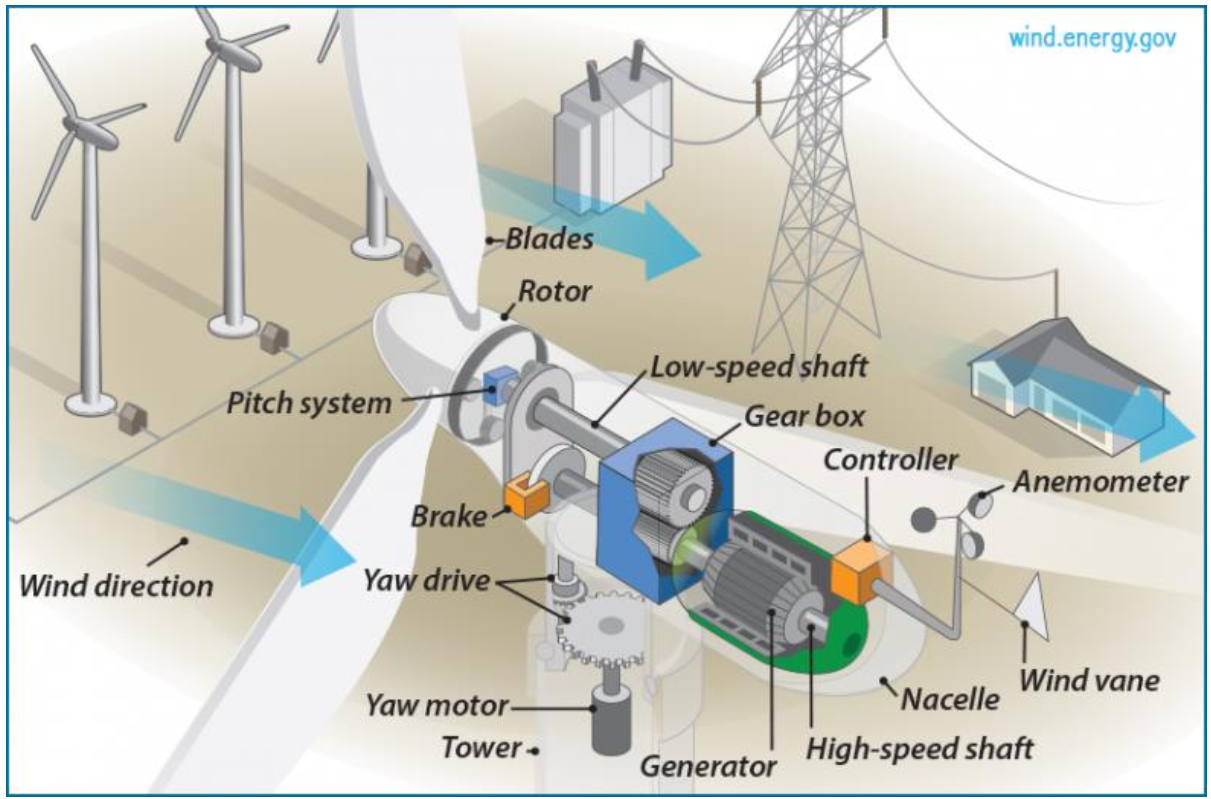
\includegraphics[width=0.7\linewidth]{Graphics/WtComponents.png}
	\caption{Illustration with an overview of the main components which make up a wind turbine}
	\label{fig:wt_components}
\end{figure}


\subsection{The floating offshore wind turbine} \label{sec:intro_theFOWT}
Floating turbines are characterized by having a floating foundation in contrast to the fixed-bottom foundation. Many foundation concepts exist and new ones are continuously proposed but four types are mainly used currently and they are depicted in \cref{fig:floating_concepts}. Each floater type is categorized based on which force is the main driver in keeping the turbine upright in the face of external forces.
\begin{figure}[ht]
	\centering
	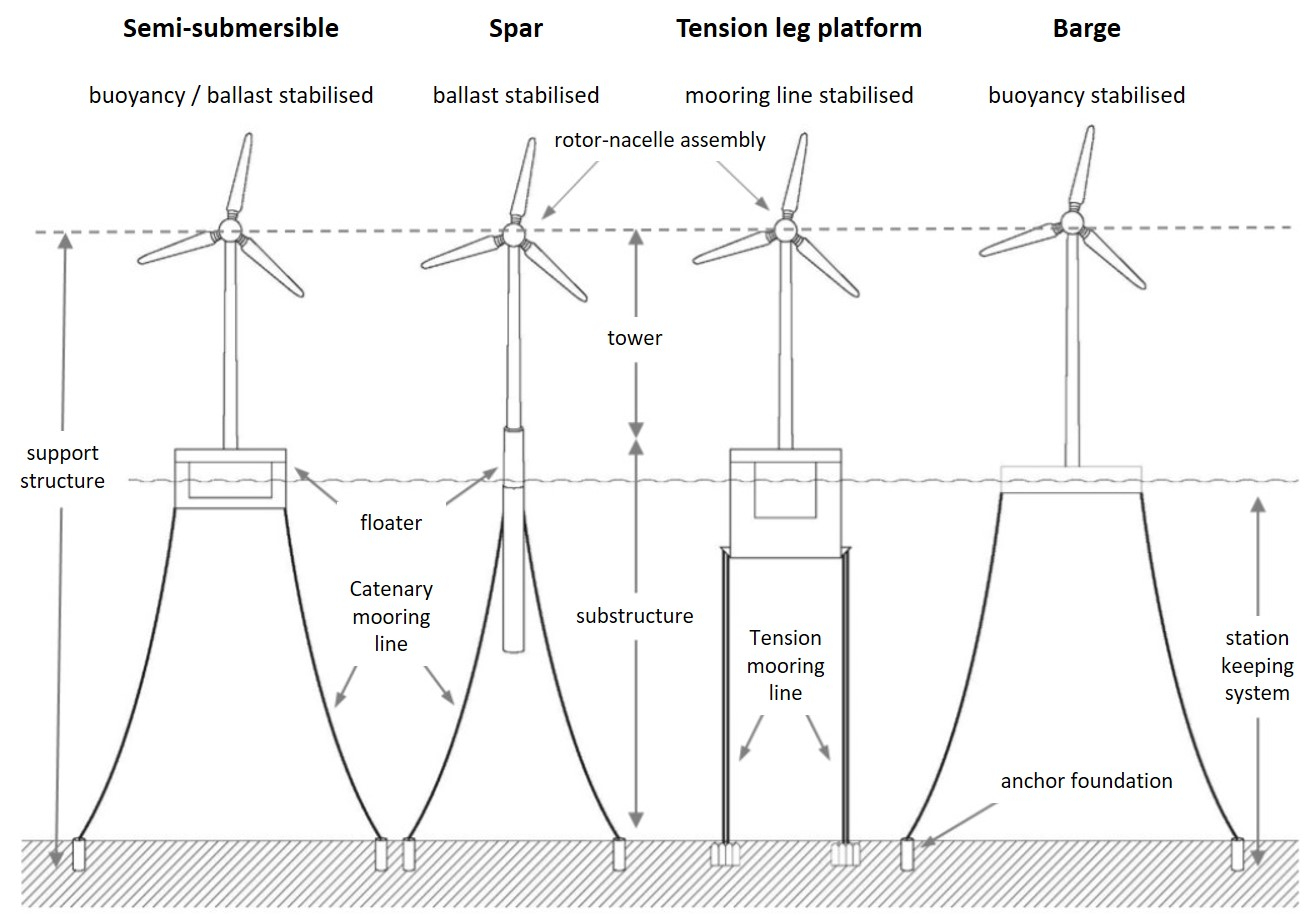
\includegraphics[width=1\linewidth]{Graphics/FloatingFoundationConcepts.jpg}
	\caption{The four main floating foundation concepts: Semi-submersible, Spar boyo, Tension leg platform and the Barge \cite{DNV-GL2018}}
	\label{fig:floating_concepts}
\end{figure}
A characteristic property of floating platforms is static stability which ensures that the overturning moment from the external loads is counteracted. The restoring force can be expressed as a sum of three components: The buoyancy force, the ballast force and the mooring line force where
\begin{itemize}
	\item the \textbf{buoyancy force} is the buoyancy contribution which is dependent on the area of water occupied by the floater
	\item the \textbf{ballast force} is the ballast contribution which is dependent on the distance from the centre of gravity and the centre of buoyancy of the platform.
	\item the \textbf{mooring line} force is the mooring line system contribution.
\end{itemize}
Foundation types in which the buoyancy contribution prevails are called buoyancy-stabilized. Likewise foundations where the ballast and mooring line contributions prevail are ballast and mooring line stabilized respectively. The semi-submersible type is both buoyancy and ballast stabilized. It achieves buoyancy stability by covering a large water-plane area and ballast stability from having three cylinders connected by struts containing ballast weights at the base. Furthermore \textit{heave plates} sit at the bottom of the cylinders yielding increased dampening while adding mass to the system.
Floaters are subjected to additional external loads: Hydrodynamic forces act on the foundation and are comprised of contributions from waves, buoyancy forces and viscous forces. The mooring system will furthermore affect the foundation and differently depending on the type of mooring system.

\smallskip
FOWTs are still in the developmental stage with a higher LCOE than the on- and offshore counterparts. They experiences greater structural strain because of significant rotational and translational motions of the support structure. The illustration in \cref{fig:fowt_coordinates} shows the additional degrees of freedom (DOFs) of FOWTs.
\begin{figure}[ht]
	\centering
	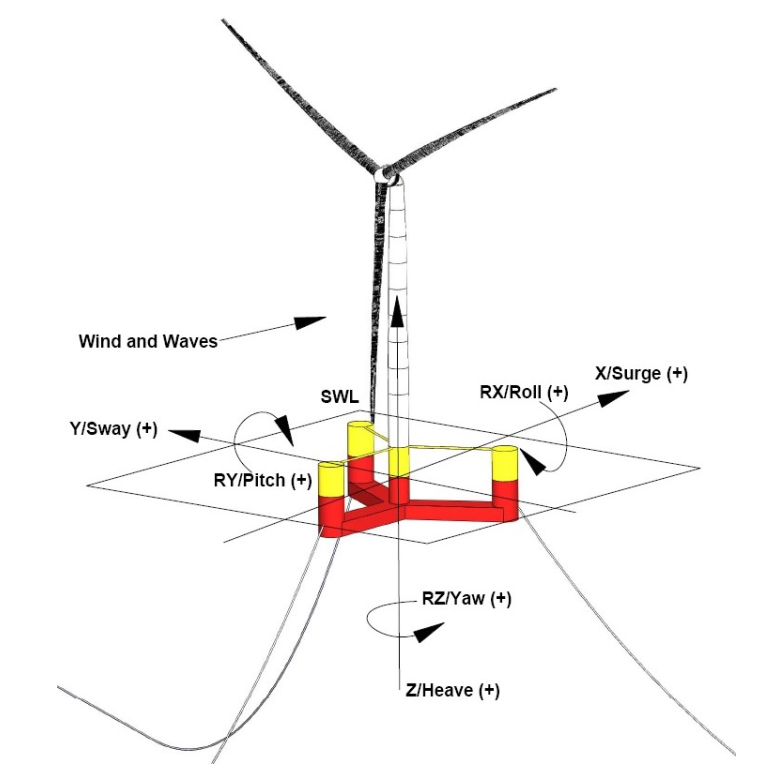
\includegraphics[width=0.55\linewidth]{Graphics/FOWTcoordinates.png}
	\caption{The 6 additional degrees of freedom (DOFs) of a floating offshore wind turbine. Figure is from internal LaC department material made by Thea Vanelli.}
	\label{fig:fowt_coordinates}
\end{figure}
Because of the increased movement, the tower is reinforced to handle the greater loads which increases the LCOE. Therefore it is of great interest to explore methods to dampen the movement of the floating WT structure. One of the large challenges in the FOWT development is handling the negative dampening problem. It is briefly described here and will be examined in greater detail in a later section.

\smallskip
As the wind is flowing through the rotor plane the wind thrusts and pitches the WT backwards. This motion is referred to as the \textit{fore-aft motion}. The backwards thrust changes the relative velocity as seen by the rotor. When the turbine moves backwards the relative wind speed decreases resulting in a decreased torque and thrust. Above nominal wind speeds the WT controller will regulate the rotor speed via the rotor pitch angle which will pitch the blades into the wind to increase the rotational speed. This increases the thrust making the WT move backwards even faster. In the forwards motion the opposite occurs where the pitch is increased to lower the rotor speed which results in an even faster forward motion. The objective of this report is to derive a linear model of a FOWT to use as a control model for reducing the fore-aft motion. 


\subsection{Problem definition} \label{sec:intro_problemdef}
Can a state-space controller, applied to a linear control model be used to reduce the fore-aft motion of a floating offshore wind turbine at an operating point? (Subject to change!)

Can a linear model at an operating point capture the dynamics of the FOWT fore-aft movement well enough to be used in a controller to dampen said motion.

- Fjern state-space
- Kan model .. enkapsle fore-aft bevægelse .. bruges til en controller
- Valideres i VTS


\newpage

% SYSTEM DESCRIPTION
% ---------------------------
\section{System Description} \label{sec:sys-descr}


% MODELING
% ---------------------------
\section{Modeling} \label{sec:mod} % Incl. Subsection "Component Models"

\subsection{Component Models} \label{sec:mod_something}

% CONTROLLER DESIGN
% ---------------------------
\section{Controller design} \label{sec:ctrl-design}
The main purpose of this chapter is firstly to present the basic LQR and LQI theory and secondly the derived LQI controller. Finally the LQI controller's effect on the system is analysed with respect to how the closed loop system poles move when LQI weights are changed.

\subsection{Linear-Quadratic Regulator} \label{sec:ctrl_lqr}
The Linear-Quadratic Regulator (LQR) in its \textit{infinite horizon} form is the preferred controller. \todo[inline]{Jesper syntes ikke at dette er god argumentaiton da han mener at den netop IKKE er intuitiv.}It is chosen because the LQR tuning process of choosing weights to penalize state deviations is deemed more intuitive than defining pole locations in the \textit{pole placement method}. Furthermore an LQR controller guarantees 6 dB gain margin and 60 degree phase margin \cite{Doyle1978}. 

\smallskip
\noindent Consider the system:
\begin{equation}\label{eq:ctrl_sys}
	\begin{split}
		\dot x &= A x + B u \\
		y &= Cx
	\end{split}
\end{equation}
For such a system the LQR controller is optimal with respect to a relevant cost function such as:
\begin{equation}\label{eq:lqr_cost}
	J = \int_{0}^{\infty} \left(x^T Q x + u^T R u + 2x^T N u\right) dt
\end{equation}
where
\begin{center}
	\begin{tabular}{l r l }
		weight & $R$         & $ > 0$\hspace{1mm} (positive definite) and symmetric       \\
		weight & $Q$ and $N$ & $\ge 0$\hspace{1mm} (positive semi-definite) and symmetric
	\end{tabular}
\end{center}
\smallskip
The final cross-term which punishes combinations of inputs and states is usually omitted by setting $ N = 0 $. The entries of $ R $ and $ Q $ are considered tuning parameters. The solution to the LQR control problem is the optimal control feedback $ u = -Kx $ which minimizes the cost function. The LQR controller is thus inherently a regulator meaning that it drives the system states to 0. For a system linearised at an operating point $ \{x_o, u_o\} $ the state and input deviations from the operating point replaces the actual states and inputs: $ \hat x = x-x_o $ and $ \hat u = u-u_o $. Given that the operating point is located at the reference, the regulator property is obviously not unattractive. With $ N = 0 $ and states substituted with state deviations the final continuous-time cost function becomes:
\begin{equation}\label{eq:lqr_cost_final}
	J = \int_{0}^{\infty} \left(\hat x^T Q \hat x + \hat u^T R \hat u\right) dt
\end{equation}
The optimal feedback gain can be shown to be: 
\begin{equation}\label{eq:lqr_K}
	K = -R^{-1} B^T P
\end{equation}
with P being the solution to the algebraic Ricatti equation:
\begin{equation}\label{lqr:ricatti}
	A^T P + P A - P B R^{-1} B^T P + Q = 0
\end{equation}
It is noted that proving \cref{eq:lqr_K} is deemed outside the scope of this report. This leaves $ Q $ and $ R $ to be tuned in such a manner that a satisfactory performance is achieved. For initial guesses \textit{Bryson's Rule} can be utilized. It states that a diagonal entry in $ Q $ or $ R $ for a corresponding state $ x_i $ or input $ u_i $ should be set as such:
\begin{equation}\label{eq:bryson}
	\begin{split}
		Q_i = \dfrac{1}{Max(\hat x_i)^2} \\
		R_i = \dfrac{1}{Max(\hat u_i)^2}
	\end{split}
\end{equation}
where $ Max(\hat x) $ is the largest tolerated value of $ \hat x $. While optimal performance is rarely achieved without further tuning, Bryson's Rule gives a good starting point. In Matlab the \textit{lqr(A, B, Q, R, N)} function is used to get the controller gains $ K $.


\subsection{Linear-Quadratic Integrator} \label{sec:ctrl_lqi}
As described \cref{sec:comp_flc} the FLC controller is of the proportional-integrator (PI) type which ensures no generator speed steady state error due to integral action. The controller to be derived includes generator speed control and the regular LQR controller does not have integral action. Therefore the system is augmented with an integral state on the generator speed $ \dot x_i = \hat \omega $ leaving the extended state space system to be:
\begin{align} 
	\dot {\bar x} & = \begin{bmatrix} \dot{\hat x} \\ \dot x_i \end{bmatrix} = \begin{bmatrix} A &0 \\ C_{iy} & 0 \end{bmatrix} \bar x + \begin{bmatrix} B_u \\ 0 \end{bmatrix}  \hat u \\
	\bar y & = \begin{bmatrix} C & 0 \end{bmatrix} \bar x
\end{align}
where $ C_{iy} $ is defined such that the desired output is picked out for integration and $ \bar x $ is the deviation state vector extended with the integral state.

A linear quadratic integrator (LQI) controller is obtained when the integrator-augmented system matrices are used to solve the LQR problem. The dimension of $ Q $ increases for every extra integrator state and thus extra weights are defined for these. While Bryson's Rule is utilized for more intuitive definitions of weights on states and inputs, the integrator state weight is a far more awkward weight to choose. In this report it is set based on a tuning process as a multiple of the original state.


\subsection{The controller} \label{sec:ctrl_thecontroller}
In the preceding sections the LQR and LQI controllers were explained and we are therefore ready to make the LQI controller. Firstly the FLC controller is removed from the system such that the input to the system is the pitch reference $ thRef $ instead of the rotor speed reference $ wRef $. Stability and controllability are checked and the system is both stable and controllable. The \textit{lqr()} Matlab function is used with the integrator-augmented system. Bryson's Rule is used to define $ Q $ and $ R $ by defining maximum limits to the states and controllable inputs. A less intuitive weight is put on the integrator state. After a controller tuning process in VTS the resulting gains are:
\begin{equation}\label{eq:lqi_K}
	K = \begin{bmatrix} -1.264 &  1.249 & -75.159 & -9.549 \end{bmatrix}
\end{equation}
when the $ Q $ and $ R $ matrices are defined as such:
\begin{equation}\label{eq:lqi_Q_and_R}
	\begin{split}
		Q = \begin{bmatrix}
			\dfrac{1}{max(p_y)^2}& 0 					& 0 															& 0 \cr
			0 					& \dfrac{1}{max(v_y)^2}	& 0 															& 0 \cr
			0 					& 0 					& \dfrac{1}{\left( max(\Omega) \cdot \frac{2 \pi}{60} \right)^2} & 0 \cr
			0 					& 0 					& 0 															& \dfrac{1}{(5 \cdot max(\Omega) \cdot \frac{2 \pi}{60})^2} \end{bmatrix} & = \begin{bmatrix}
			\dfrac{1}{5^2} 	&  	0 				&  0 										&  0 \cr
			0 				&  \dfrac{1}{1^2}	&  0 										&  0 \cr
			0 				&  0 				& \dfrac{1}{\left( 1 \cdot \frac{2 \pi}{60} \right)^2} 	&  0 \cr
			0 				&  0 				&  0 										&  \dfrac{1}{(5 \cdot \frac{2 \pi}{60})^2}
		\end{bmatrix} \\\\
		R = \begin{bmatrix} \dfrac{1}{\max(\theta_{ref})^2} \end{bmatrix} &= \begin{bmatrix} \dfrac{1}{5^2} \end{bmatrix}
	\end{split}
\end{equation}
From $ Q $ and $ R $ it is observable that:
\begin{itemize}
	\item the maximum allowed fore-aft position deviation is set to 5 m
	\item the maximum allowed fore-aft velocity deviation is set to 1 m/s
	\item the maximum allowed rotor speed deviation is set to 1 rpm
	\item the rotor speed integration weight is set 5 times lower than the rotor speed
	\item the maximum allowed pitch angle actuation deviation is set to 5 deg
\end{itemize}
The maximum tolerated rotor speed is multiplied with $ 2 \pi $/$ 60 $ to translate the weight from rpm to rad/s which is the state unit. There is furthermore no intuitive explanation behind the choice of the integrator weight other than that it has yielded satisfactory results in the controller tuning process. Only light tuning was necessary from the initial guesses of maximum tolerable state and input values to achieve good performance. This is regarded as a highlight of the usefulness of the LQR controller when a well fitting linear model is used. Also perhaps importantly when the necessary system understanding has not been achieved such that pole placement can be done based on reasonable design considerations. Some system understanding can perhaps be achieved by considering the positions of system poles and zeros and thus a drawback of LQR might be that some understanding is lost when omitting this process.
%\begin{equation}\label{eq:lqi_Q_and_R}
%	Q =   \begin{bmatrix}
%		0.04 &  0 &  0 &  0 \cr
%		0 &  1 &  0 &  0 \cr
%		0 &  0 & 91.1 &  0 \cr
%		0 &  0 &  0 &  3.65
%	\end{bmatrix}
%	 \;\; and \;\; 
%	R = \begin{bmatrix} 0.04 \end{bmatrix}
%\end{equation}



%s_W = 1; s_py = 5; s_vy = 1; s_Wi = s_W*5; s_th = 5;
%var_Omega	= (s_W * (2*pi)/60)^2;	% Permitted variance of Omega in [rad/s]
%var_py		= s_py^2;				% Permitted variance of py in [m]
%var_vy		= s_vy^2;				% Permitted variance of vy in [m/s]
%Qlqr = [1/var_py	0			0
%0			1/var_vy	0
%0			0			1/var_Omega];


%\begin{equation}\label{eq:lqi_Q_and_R}
%	Q =   \begin{bmatrix}
%		\dfrac{1}{5^2} 	&  	0 				&  0 										&  0 \cr
%		0 				&  \dfrac{1}{1^2}	&  0 										&  0 \cr
%		0 				&  0 				& \dfrac{1}{\left( 1 \cdot \frac{2 \pi}{60} \right)^2} 	&  0 \cr
%		0 				&  0 				&  0 										&  \dfrac{1}{(5 \cdot \dfrac{2 \pi}{60})^2}
%	\end{bmatrix}
%	\;\; and \;\; 
%	R = \begin{bmatrix} \dfrac{1}{5^2} \end{bmatrix}
%\end{equation}

\subsection{LQI controller analysis}
This section is dedicated to analysing how the LQI controller moves the system poles and changes the system behaviour when some weights of $ Q $ and $ R $ are changed. The poles of the open-loop uncontrolled system is plotted together with the closed-loop LQI controlled system. Each plot contains a change in one weight (e.g. via $ max(\Omega) $) with three variations of that weight to see how the poles move. The weights which are not changed are left at the tuned values presented in \cref{sec:ctrl_thecontroller}. 

\smallskip
In \cref{fig:pzmap_vy} the LQI $ Q $ weight on $ v_y $ is varied via $ 1/max(v_y)^2 $. The blue markers indicate the poles of the uncontrolled system. The frequency of the pole pair closest to the imaginary axis fit well with the structure eigenfrequency around 0.035 Hz. The high ratio between the imaginary and real part indicate a very low dampening of especially the uncontrolled system (blue markers). As expected when putting a greater constraint on the tower velocity the dampening is increased. It moves from 0.28 for $ max(vy) = 1 $ to 0.435 for $ max(vy) = 0.25 $. This happens because of the reduction of mainly the imaginary component of the dominating pole pair. The increased dampening is expected to lead to reduced oscillations of the turbine structure. This is also apparent when observing a step response as in \cref{fig:step_vy}. Here a reduction of the oscillations of $ p_y $ and $ v_y $ is observed but at the cost of a greater rotor tracking error. Furthermore, in the pole-zero diagram, the \textit{fastest} (most negative) pole on the real axis becomes even faster while the slowest becomes slower. The implications of how this affects the system response is harder to deduce. It is especially difficult to reason why the pole movement translates into the observed rotor speed response.

Furthermore one might wonder why the LQI controller does not simply make the dominating floating pole pair even faster with an even higher dampening. Here one should consider that a constraint on the actuator effort is still in place (in the form of $ max(\theta_{ref}) = 5 $) which limits the possibility of extensively reducing the fore-aft motion.
\begin{figure}[ht]
	\centering
	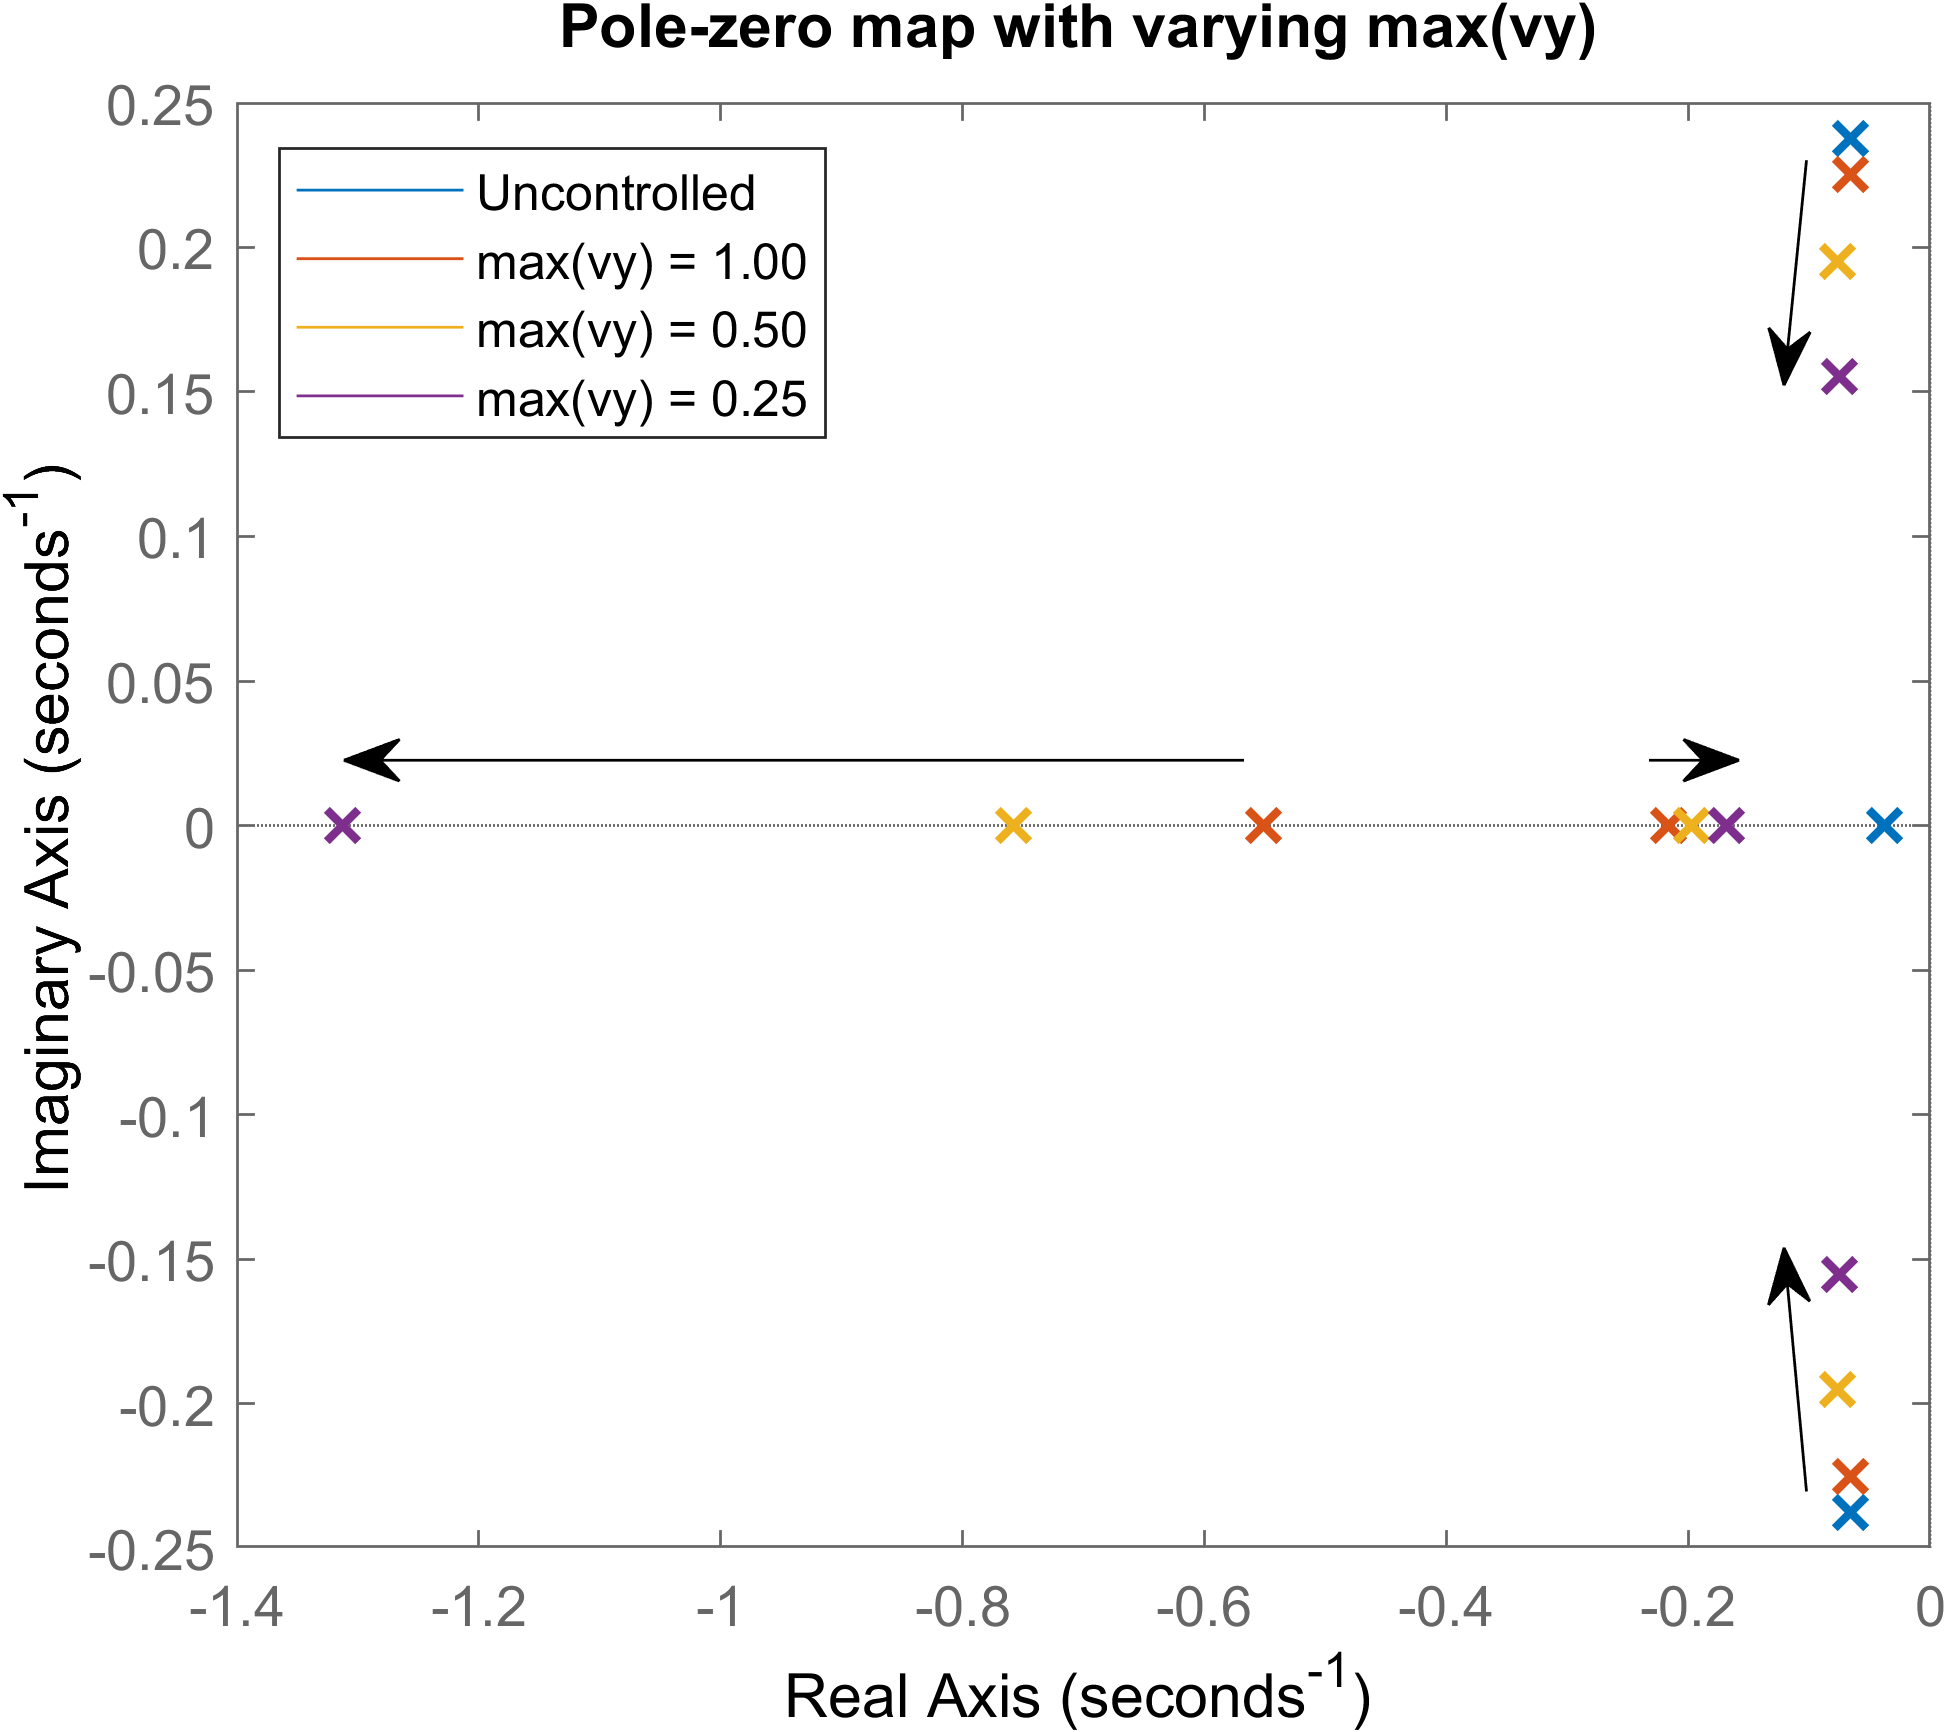
\includegraphics[width=.55\textwidth]{Graphics/LQI pole zero/02_pzmap_vy}
	\caption{Pole-zero diagram with varying LQI weight on the state $ v_y $. Arrows indicate the pole movement direction tendency.}
	\label{fig:pzmap_vy}
\end{figure}
\begin{figure}[ht]
	\centering
	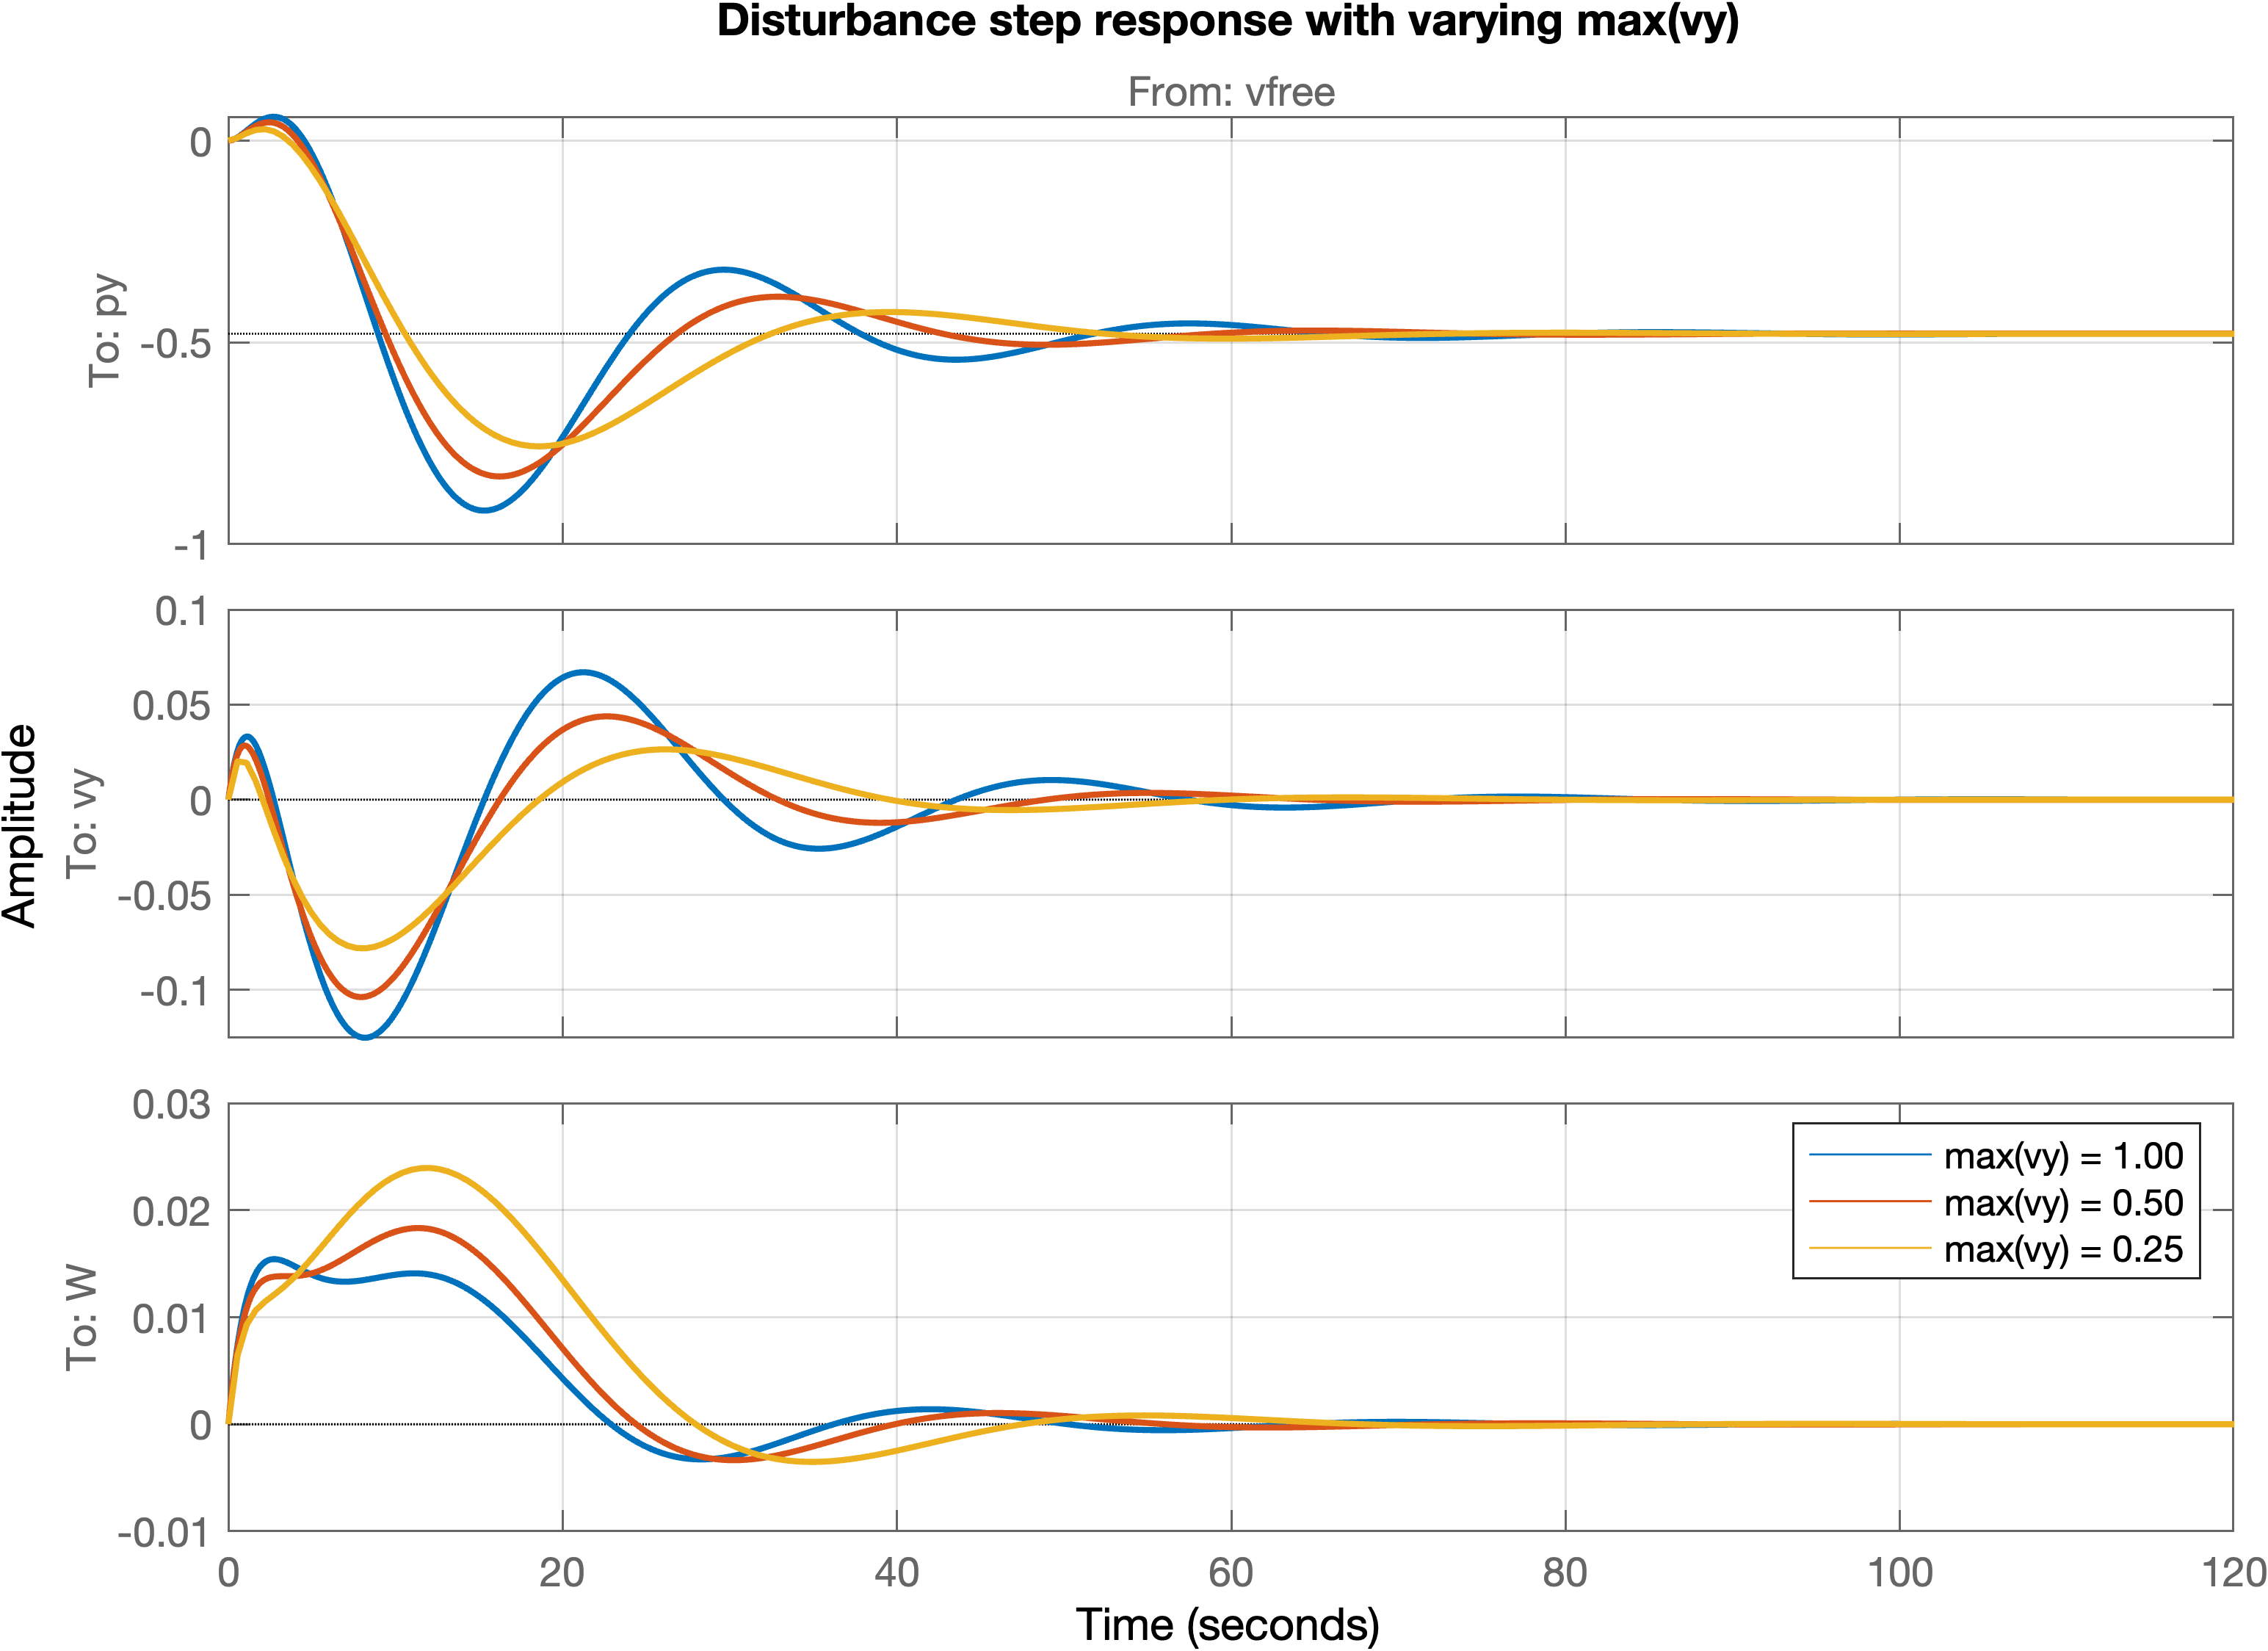
\includegraphics[width=0.7\textwidth]{Graphics/LQI pole zero/102_step_vy.png}
	\caption{Step response from a step on the free wind disturbance. The constraint on $ v_y $ is varied. The y-axis shows the deviation from the operating point. The rotor speed reference is at the operating point and therefore the third subplot shows the rotor speed tracking error. An increased constraint on the fore-aft velocity results in reduced fore-aft motion oscillations but greater rotor speed tracking error.}
	\label{fig:step_vy}
\end{figure}

In \cref{fig:pzmap_W_both} two plots are seen where the one in \cref{fig:pzmap_W_zoom} is zoomed in at the area indicated in the top right corner of \cref{fig:pzmap_W}. Here greater constraint is put on $ \Omega $ and in contrast to the $ v_y $ case the dominating pole pair of the floating structure moves in the opposite direction. This leads to lower dampening and stability of the floating movement due to the poles being closer to the imaginary axis. As expected when observing the step response in \cref{fig:step_W} the fore-aft oscillations are greater and last longer. Surprisingly the two poles located on the real axis move in the same direction as in \cref{fig:pzmap_vy} with the fastest pole becoming much faster and the slow pole becoming much slower. The effect as seen on the step response is that the rotor speed error is reduced. Giving a reasonable explanation for the movement of the poles on the real axis and how it yields better rotor speed tracking is difficult. With regards to the floating pole pair it is perhaps intuitive that if a much greater emphasis is put on limiting the rotor speed error it comes at the cost of less desirable fore-aft motion.
\begin{figure*}[ht]
	\centering
	
	\subfloat[Pole-zero map]
	{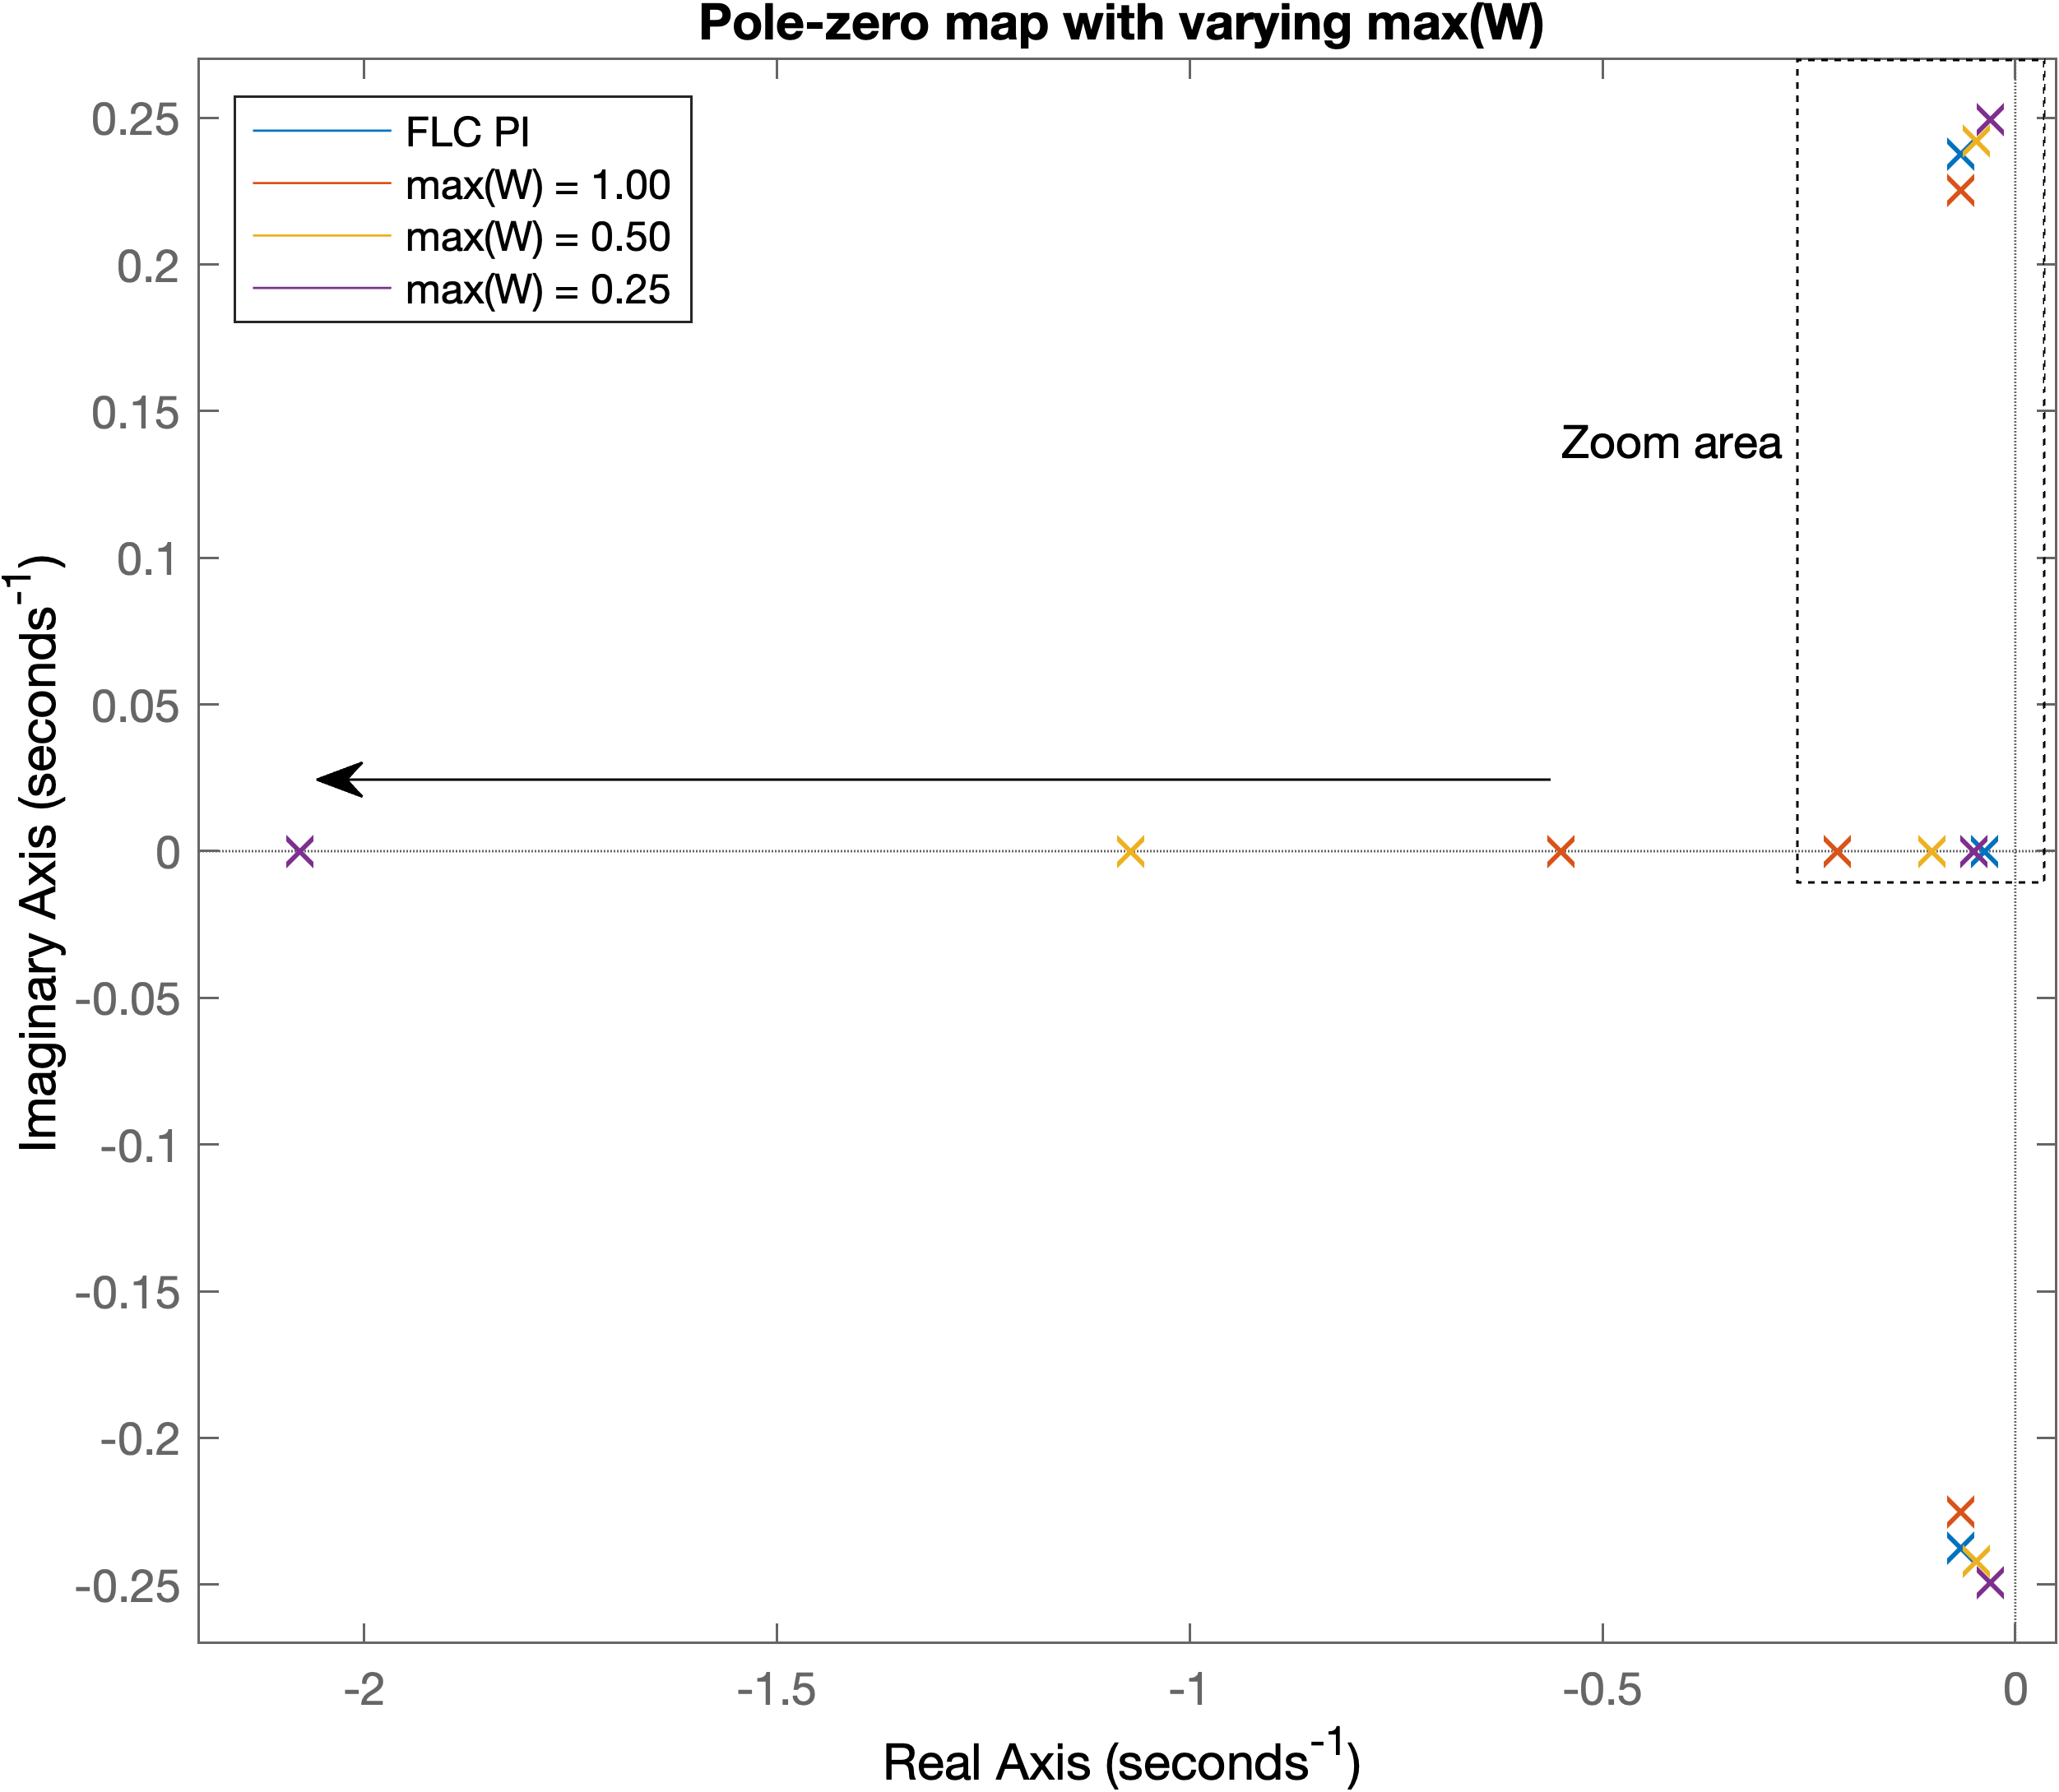
\includegraphics[width=.48\textwidth]{Graphics/LQI pole zero/03_pzmap_W}%
		\label{fig:pzmap_W}}
	\hfil
	\subfloat[Pole-zero map zoomed]
	{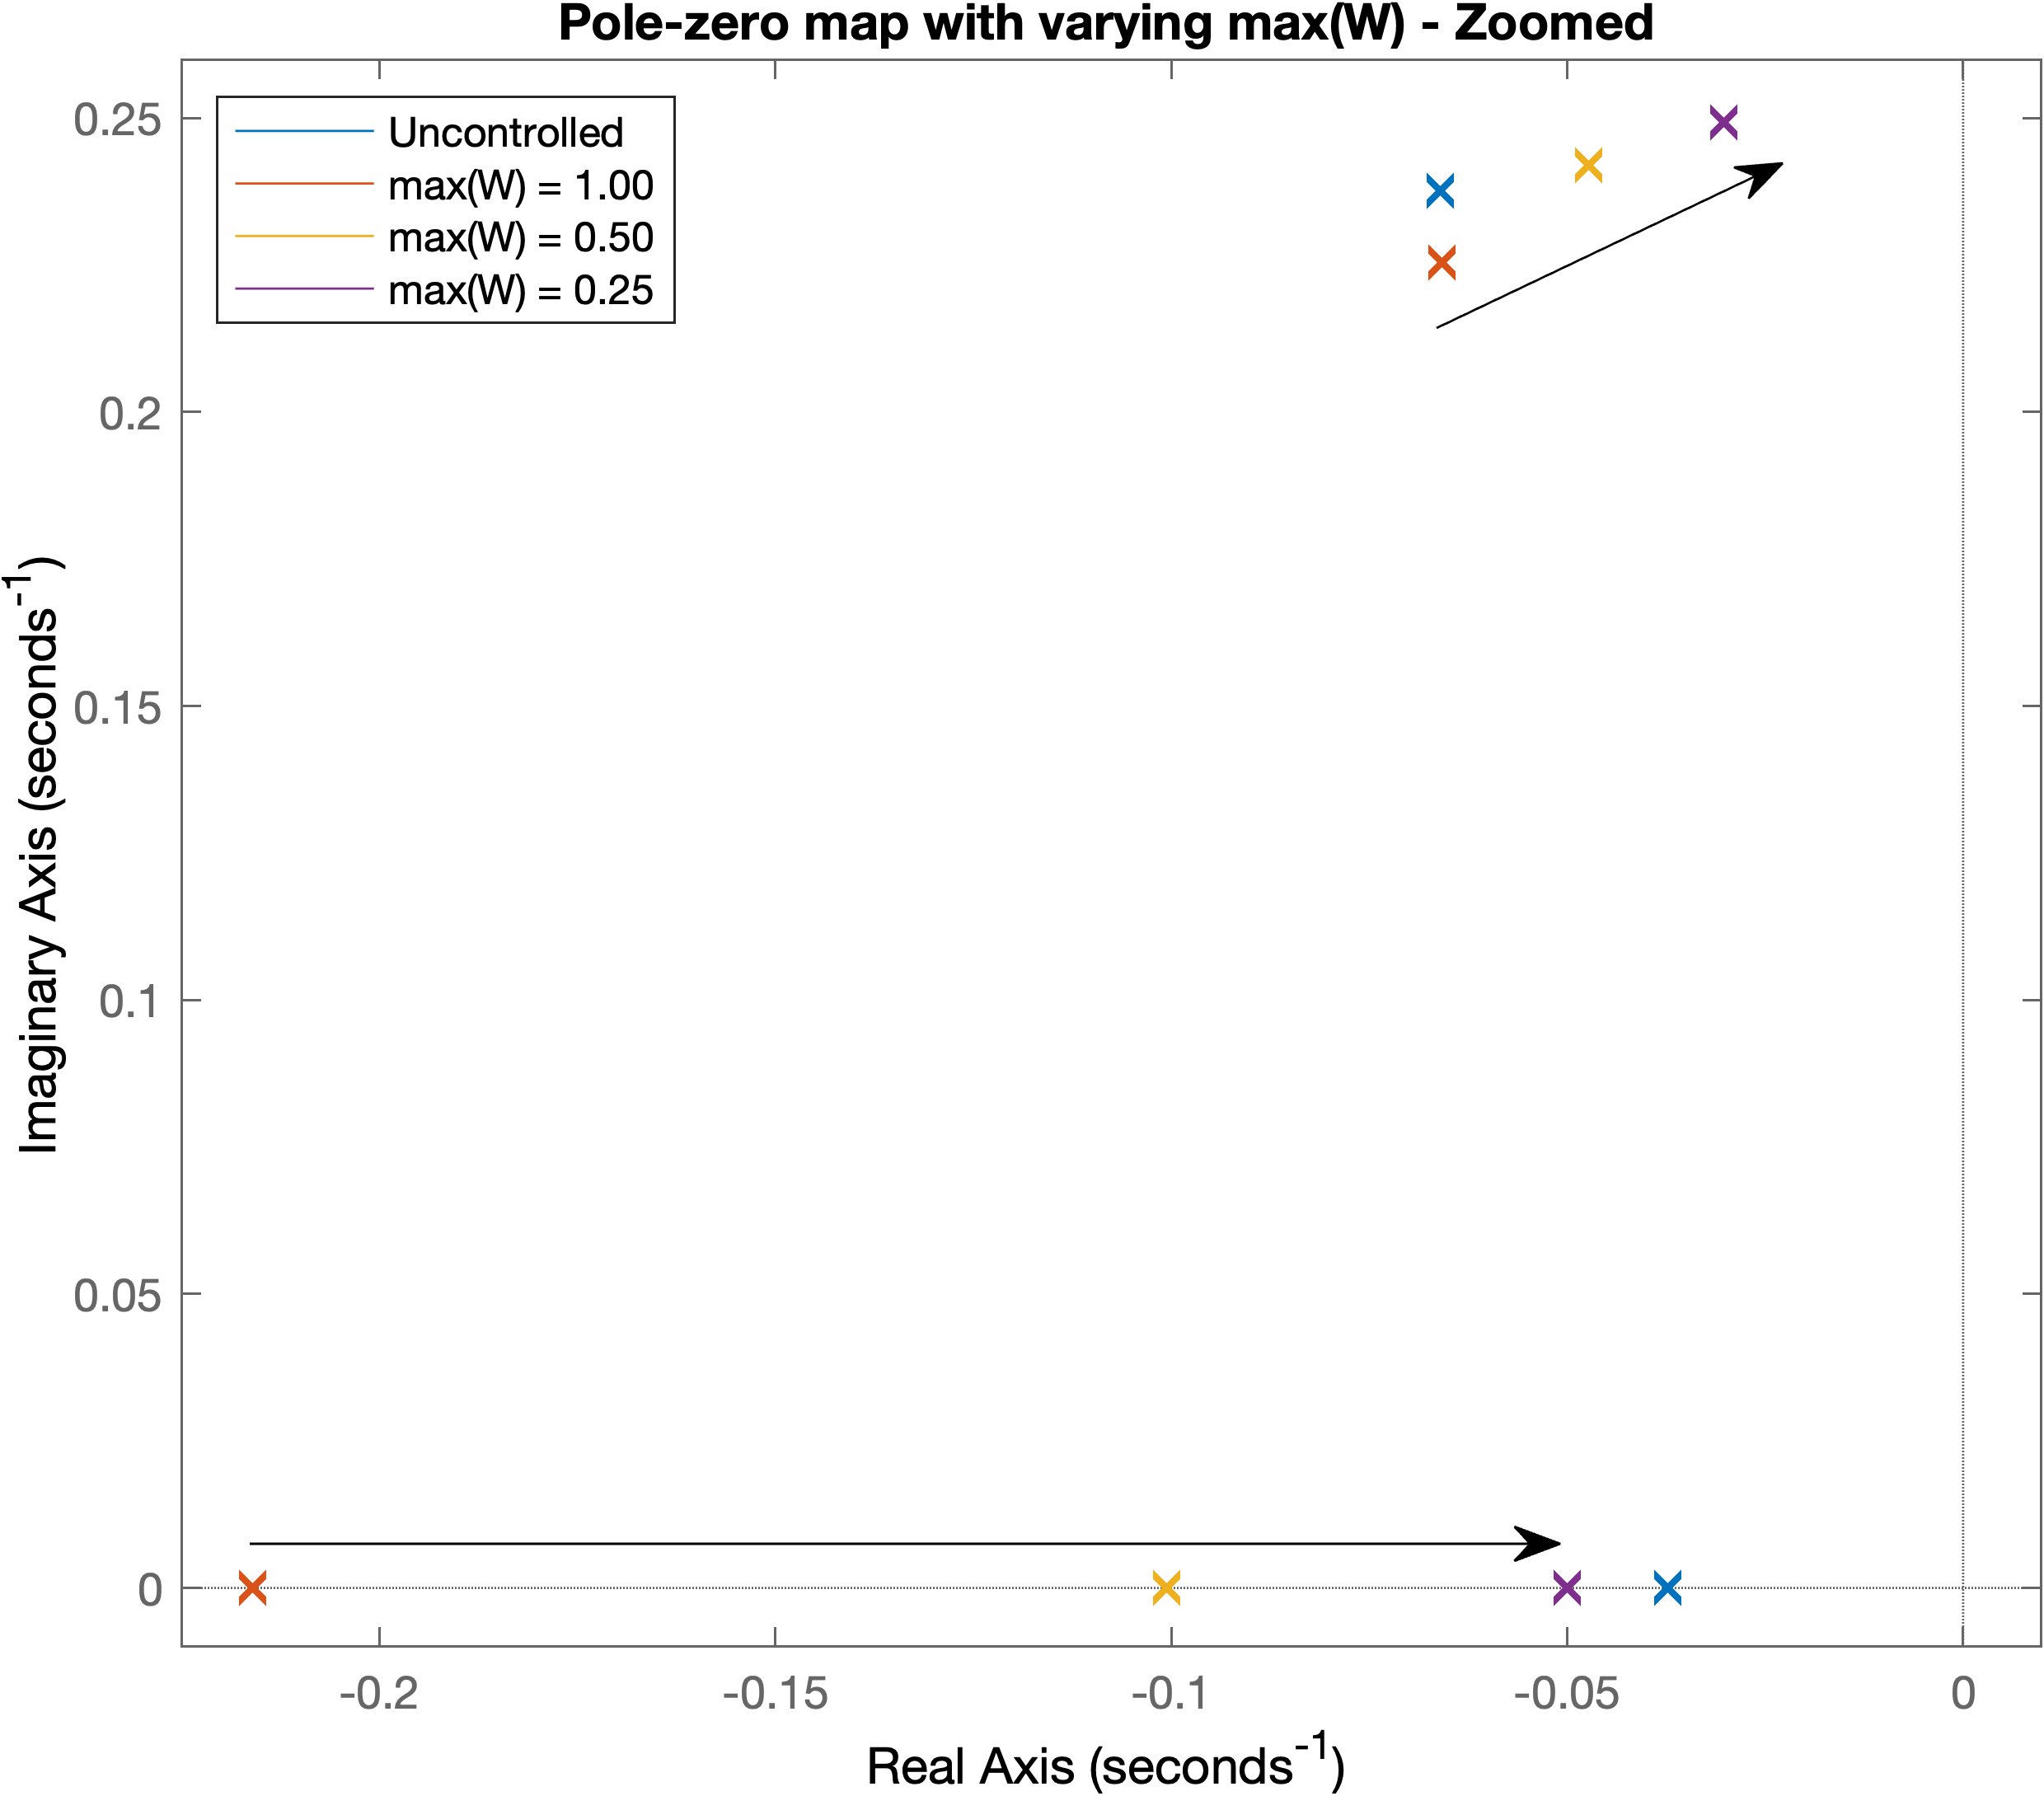
\includegraphics[width=.48\textwidth]{Graphics/LQI pole zero/13_pzmapzoom_W}%
		\label{fig:pzmap_W_zoom}}
	
	\caption{Pole-zero diagram with varying LQI weight of the state $ \Omega $; \textbf{(a)} a-text; \textbf{(b)} b-text.}
	\label{fig:pzmap_W_both}
\end{figure*}
\begin{figure}[ht]
	\centering
	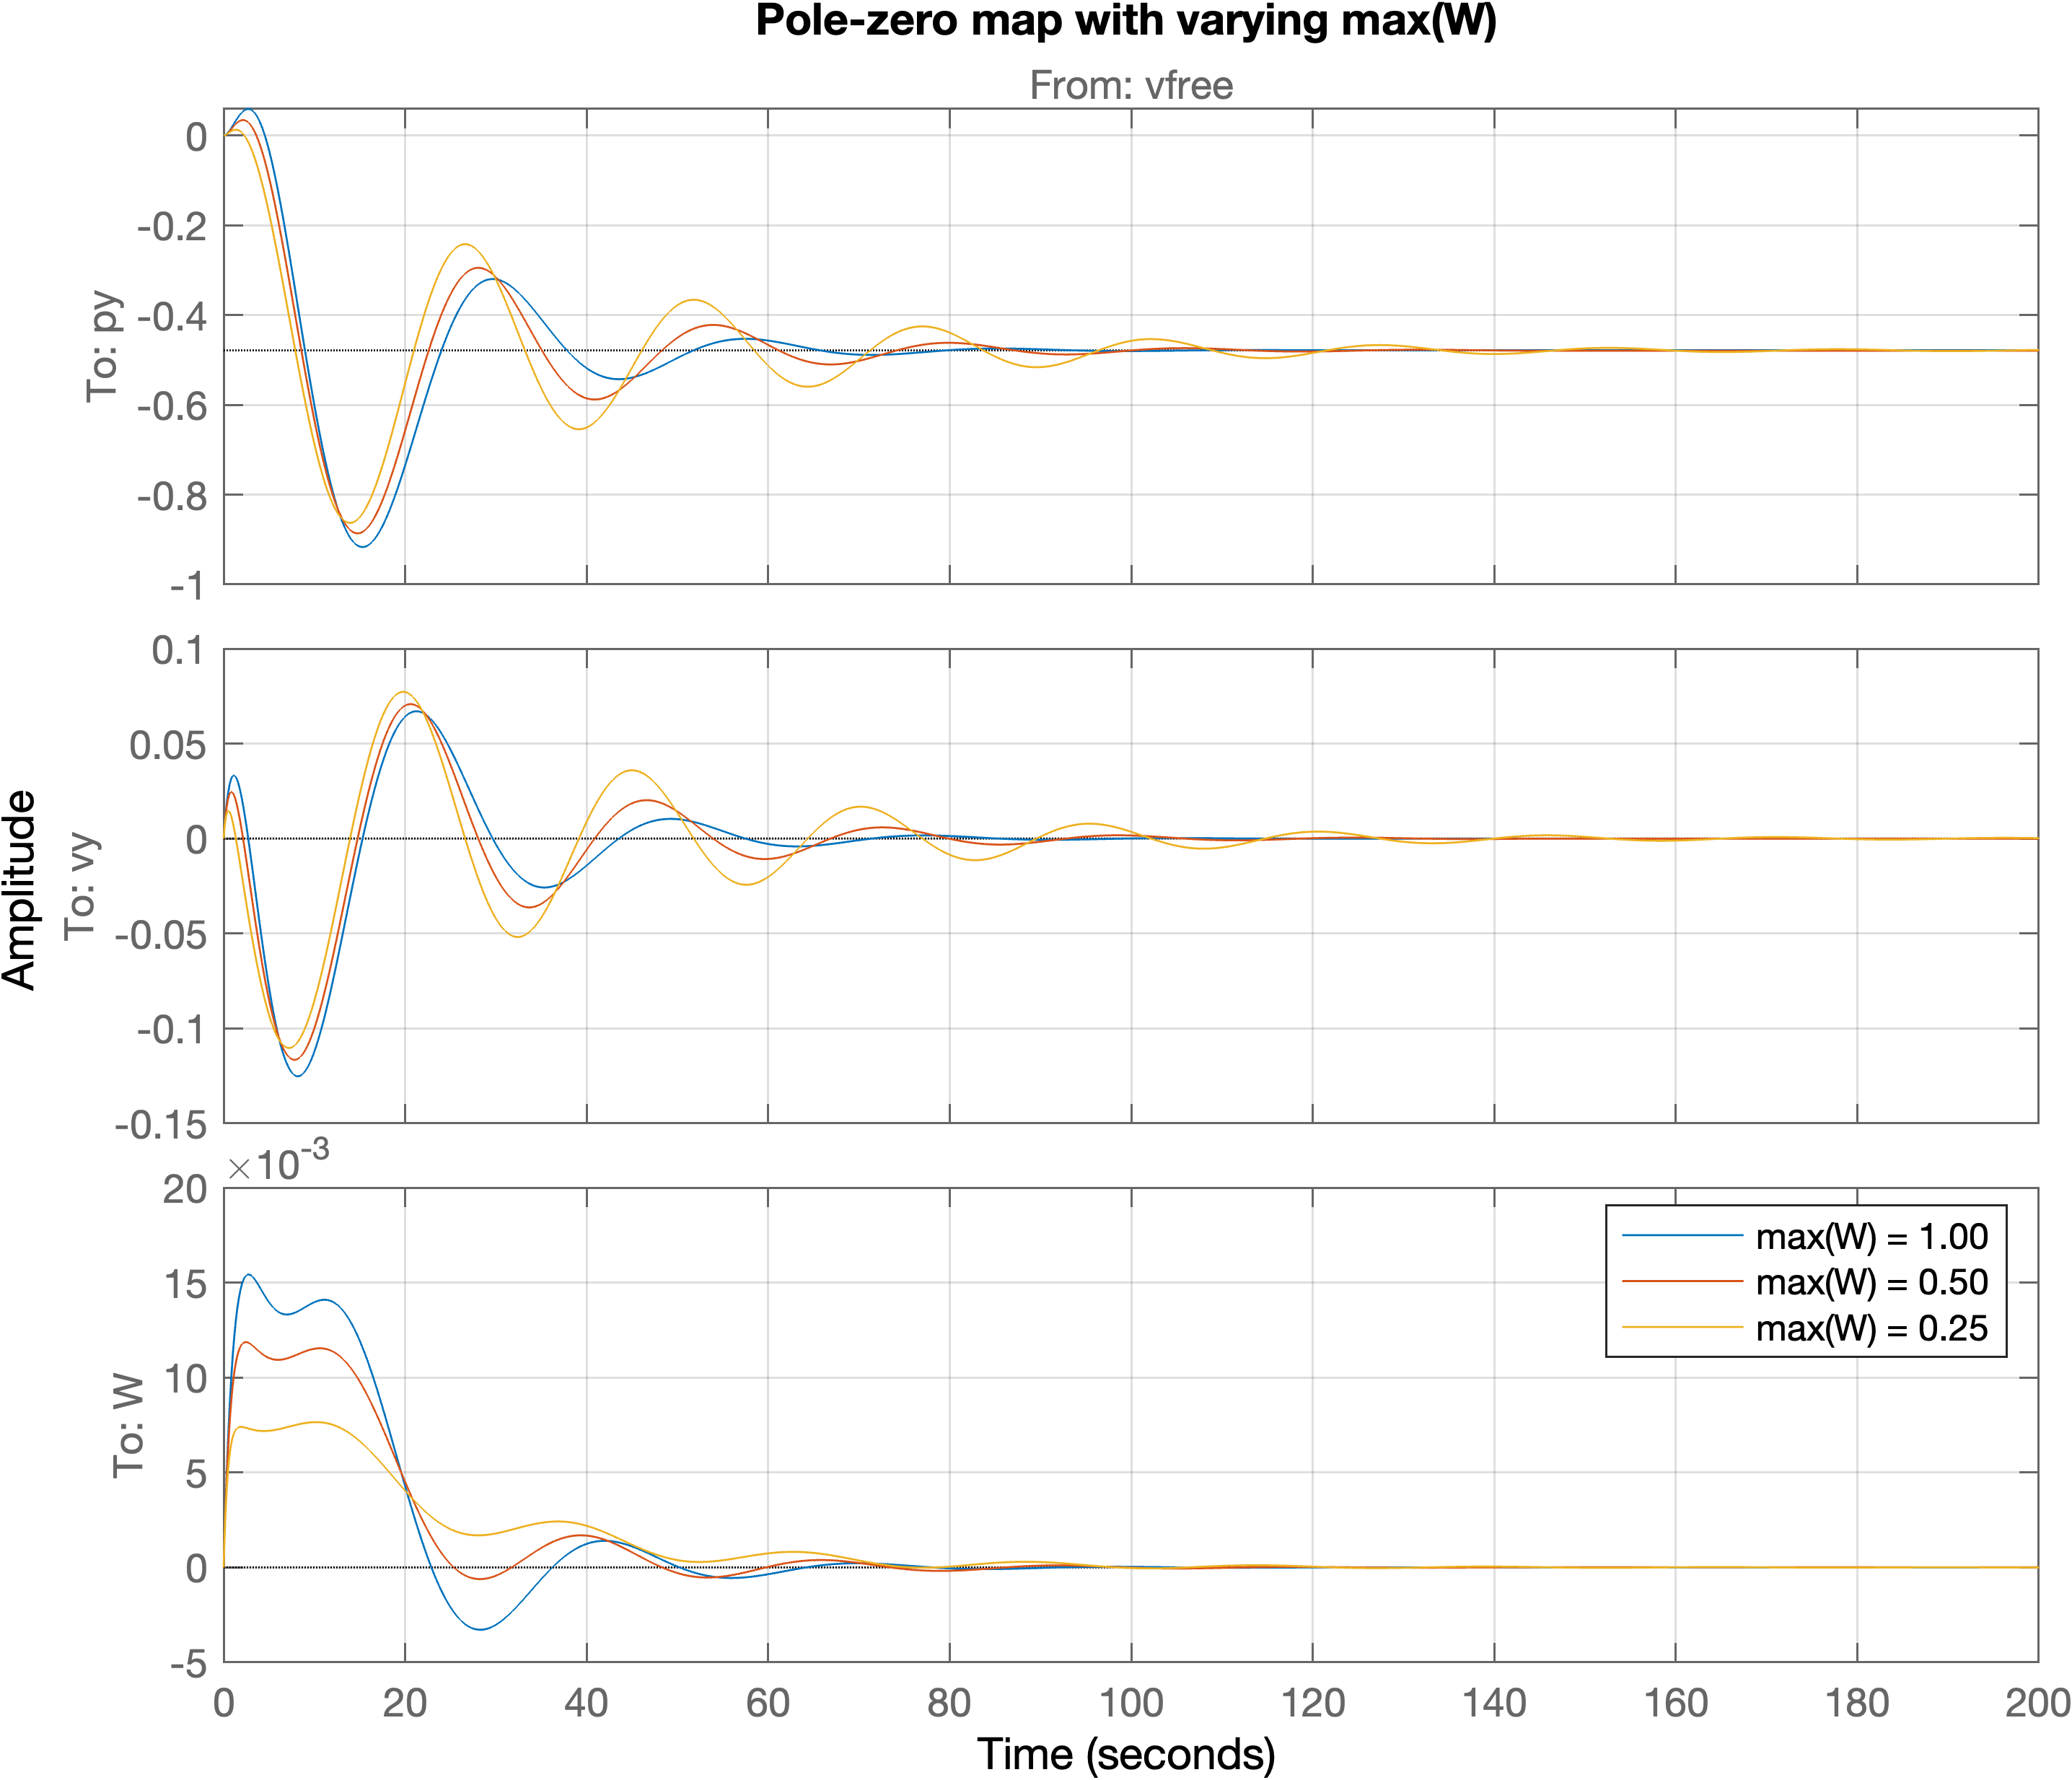
\includegraphics[width=0.7\textwidth]{Graphics/LQI pole zero/103_step_W.png}
	\caption{Step response from a step on the free wind disturbance. The constraint on $ \Omega $ is varied. The y-axis shows the deviation from the operating point. The rotor speed reference is at the operating point and therefore the third subplot shows the rotor speed tracking error. An increased constraint on the rotor speed tracking error yields slightly greater fore-aft motion oscillations but lower rotor speed tracking overshoot.}
	\label{fig:step_W}
\end{figure}

In \cref{fig:pzmap_theta} the constraint on the rotor pitch angle actuation is varied from 1 deg to 5 deg with 5 deg being the original tuned parameter. With a tight constraint on the pitch angle of 1 deg the two poles which were located at the real axis have instead become a slower pole pair as observed by the red poles at $ -0.1 \pm0.8 $. As the constraint is relieved from 1 to 5 deg the pole pair becomes faster with a lower dampening and ultimately turns into two faster real poles. The dominating pole pair's imaginary part is furthermore lowered as the constraint is relieved. The general tendency is that the system becomes both faster and more dampened. As expected allowing for a greater actuator effort leads to a better and faster system altogether which is also readily visible in the step response in \cref{fig:step_theta}. Both the magnitude of oscillations and settle time is reduces for both the tower movement and rotor speed error.
\begin{figure}[ht]
	\centering
	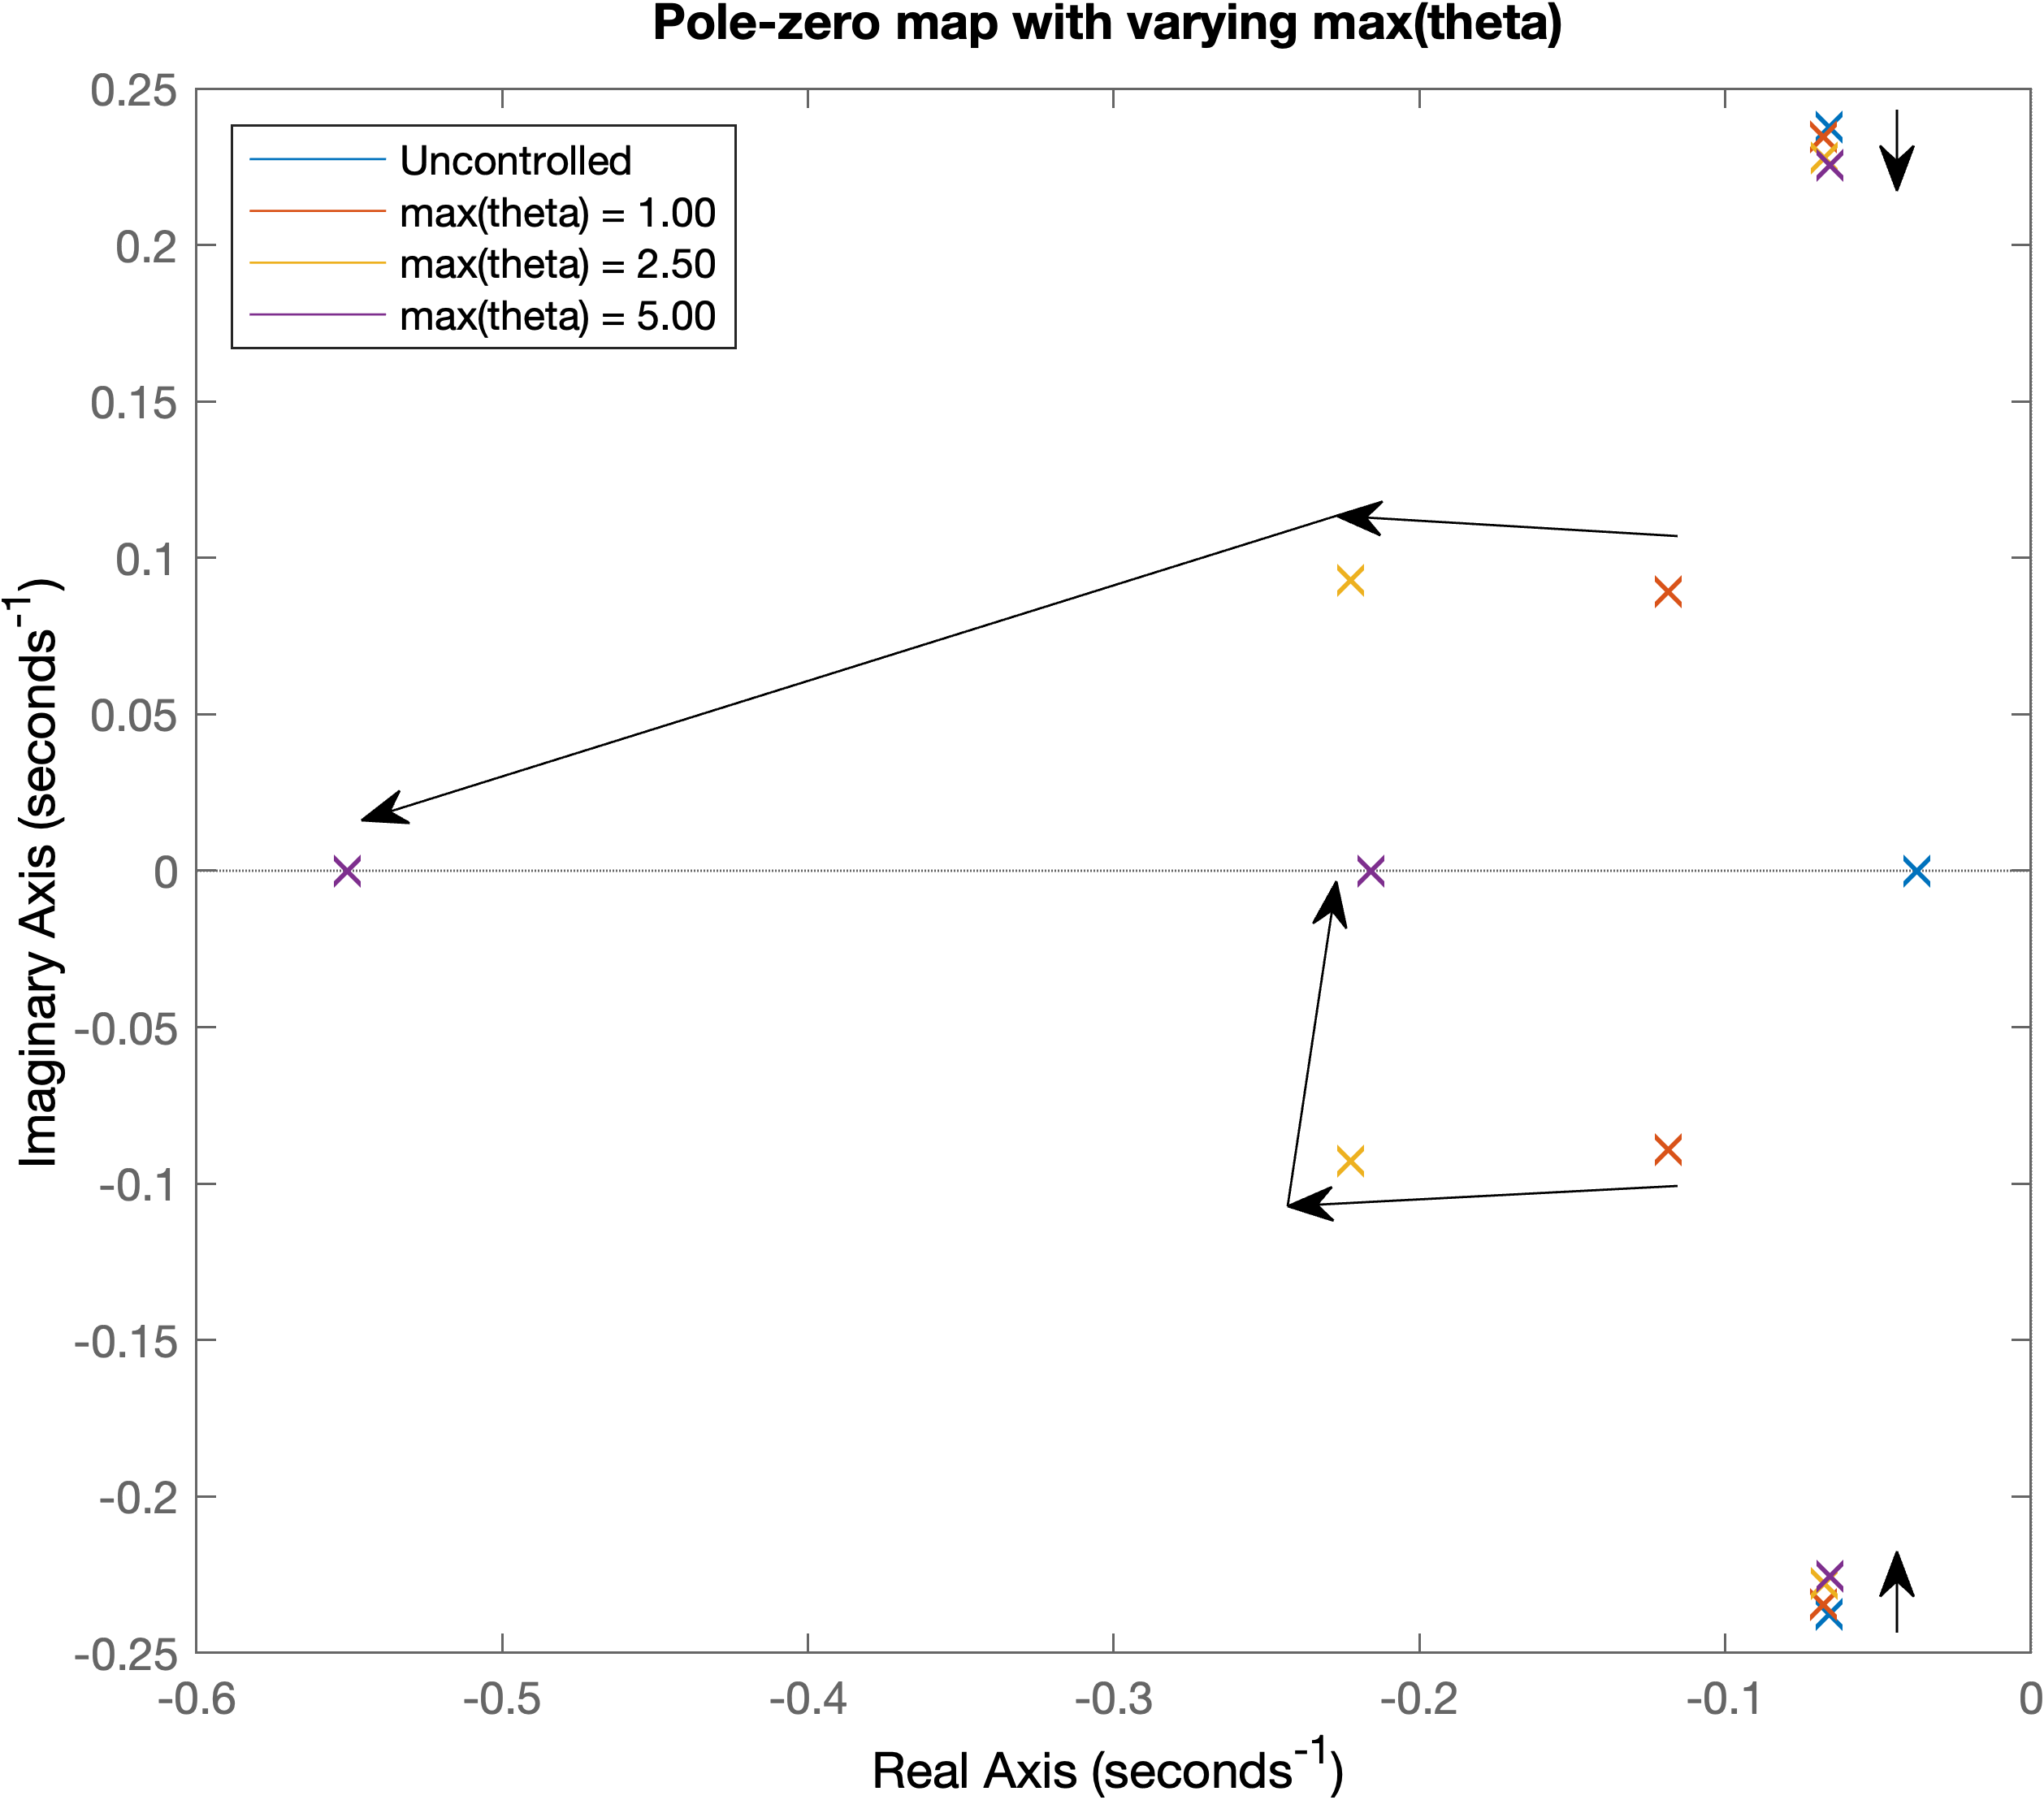
\includegraphics[width=0.55\textwidth]{Graphics/LQI pole zero/05_pzmap_theta.png}
	\caption{Poze-zero diagram with varying LQI weight on the actuator input $ \theta $}
	\label{fig:pzmap_theta}
\end{figure}

\begin{figure}[ht]
	\centering
	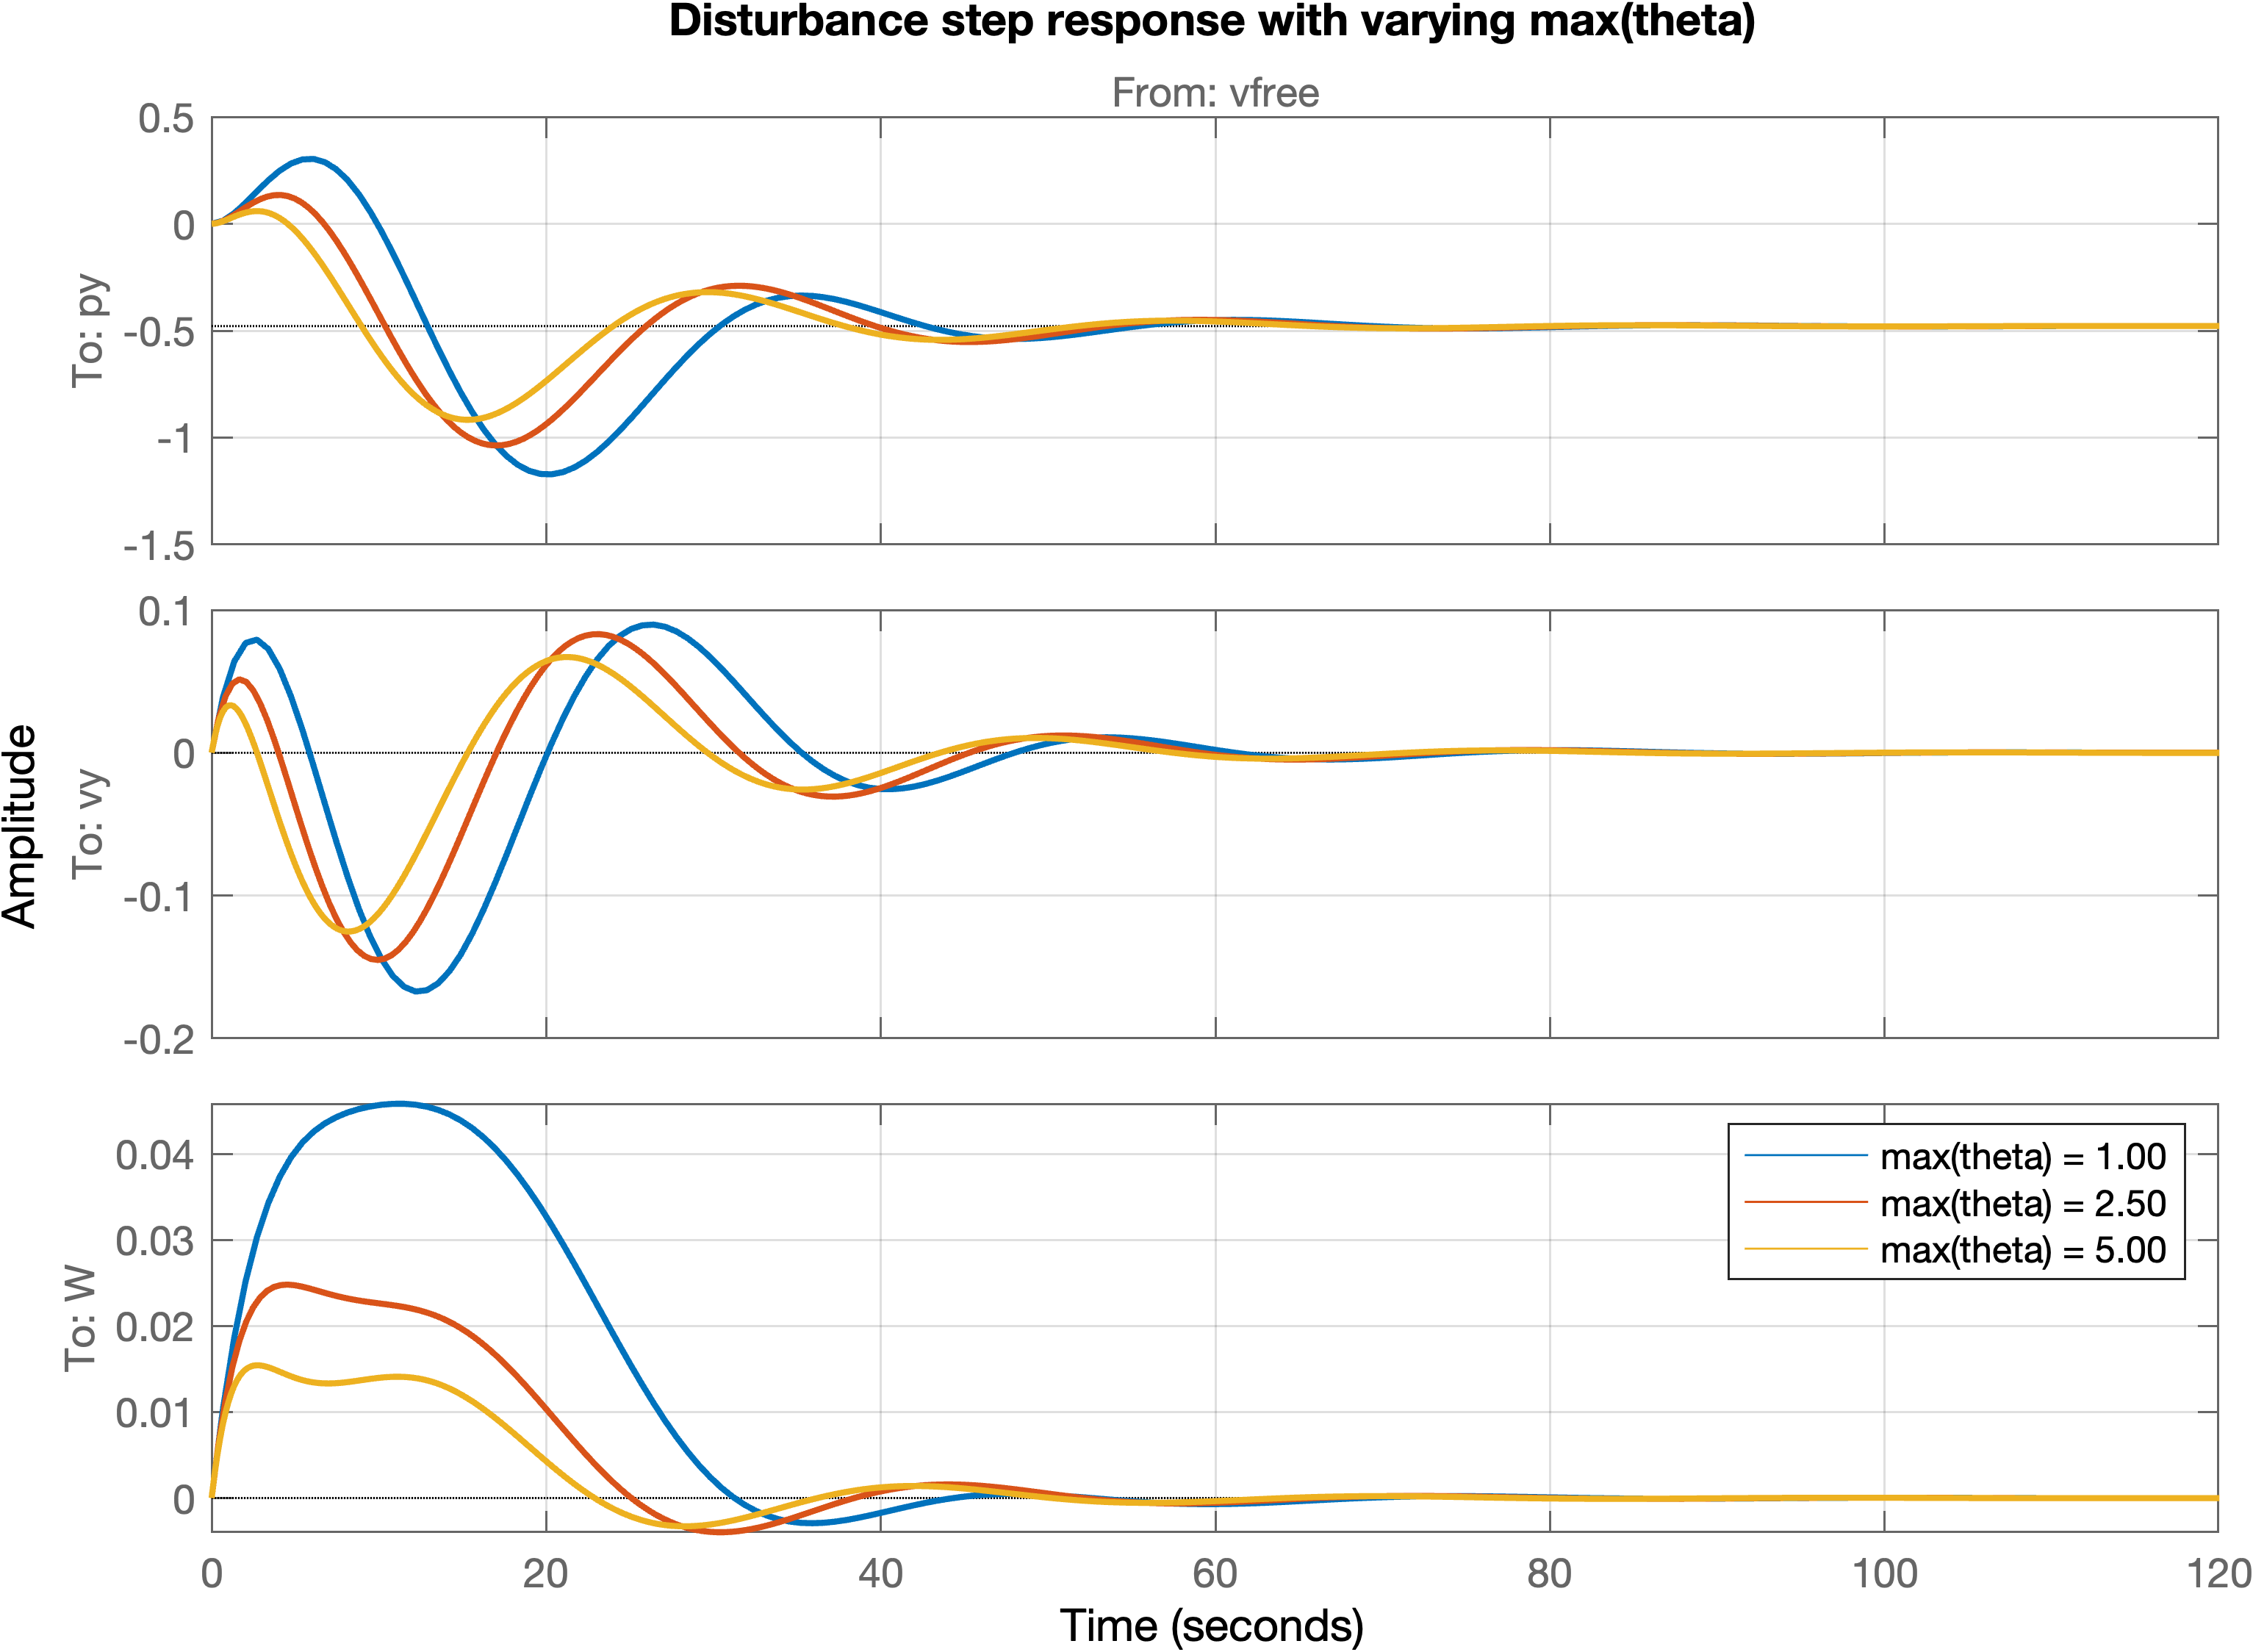
\includegraphics[width=0.7\textwidth]{Graphics/LQI pole zero/105_step_theta.png}
	\caption{Step response from a step on the free wind disturbance. The constraint on $ \theta_{ref} $ is varied. The y-axis shows the deviation from the operating point. The rotor speed reference is at the operating point and therefore the third subplot shows the rotor speed tracking error. Lowered constraints on the actuator effort results in both smaller fore-aft oscillations with lower settling time and smaller rotor speed tracking overshoot with slightly lower settling time.}
	\label{fig:step_theta}
\end{figure}


%\begin{figure*}[ht]
%	\centering
%	
%	\subfloat[sub-float1]
%	{\includegraphics[width=.49\textwidth]{Graphics/LQI pole zero/}%
%		\label{fig:1}}
%	\hfil
%	\subfloat[sub-float2]
%	{\includegraphics[width=.50\textwidth]{Graphics/LQI pole zero/}%
%		\label{fig:2}}
%	
%	\caption{Total text; \textbf{(a)} a-text; \textbf{(b)} b-text.}
%	\label{fig:3}
%\end{figure*}

% TEST - SIMULATION
% ---------------------------
\clearpage
\newpage

% TEST - REAL SYSTEM
% ---------------------------
\clearpage
\newpage

% CONCLUSION
% ---------------------------
\clearpage
\newpage
\section{Conclusion} \label{sec:concl}

\textbf{THE GOOD}

\begin{itemize}
	\item Good thing 1
	\item Good thing 2
\end{itemize}

\noindent \textbf{THE BAD}

\begin{itemize}
	\item The LQI implementation in VTS requires \textit{real} states of py and vy
\end{itemize}

\noindent \textbf{THE GOOD \#2}

\begin{itemize}
	\item Good thing 1
\end{itemize}

\textbf{Conclusion text:}
 The underlying physics of a trailer refrigeration system are complex, as several components of the system require extensive modeling to accurately represent reality. xxx














% CONCLUSION
% ---------------------------
\clearpage
\newpage
\section{Future work} \label{sec:future}

\begin{itemize}
	\item Make a gain scheduling scheme for all of the FL region: 1. tune LQI weights for a range of operating points and interpolate between them to get continuous controller parameter functions. 2. Derive an inverse function of the non-linear pitch authority. 
	\item Make an estimator for the fore-aft position and velocity
\end{itemize}

% An example of a floating figure using the graphicx package.
% Note that \label must occur AFTER (or within) \caption.
% For figures, \caption should occur after the \includegraphics.
% Note that IEEEtran v1.7 and later has special internal code that
% is designed to preserve the operation of \label within \caption
% even when the captionsoff option is in effect. However, because
% of issues like this, it may be the safest practice to put all your
% \label just after \caption rather than within \caption{}.
%
% Reminder: the "draftcls" or "draftclsnofoot", not "draft", class
% option should be used if it is desired that the figures are to be
% displayed while in draft mode.
%
%\begin{figure}[!t]
%\centering
%\includegraphics[width=2.5in]{myfigure}
% where an .eps filename suffix will be assumed under latex,
% and a .pdf suffix will be assumed for pdflatex; or what has been declared
% via \DeclareGraphicsExtensions.
%\caption{Simulation results for the network.}
%\label{fig_sim}
%\end{figure}

% Note that the IEEE typically puts floats only at the top, even when this
% results in a large percentage of a column being occupied by floats.


% An example of a double column floating figure using two subfigures.
% (The subfig.sty package must be loaded for this to work.)
% The subfigure \label commands are set within each subfloat command,
% and the \label for the overall figure must come after \caption.
% \hfil is used as a separator to get equal spacing.
% Watch out that the combined width of all the subfigures on a
% line do not exceed the text width or a line break will occur.
%
%\begin{figure*}[!t]
%\centering
%\subfloat[Case I]{\includegraphics[width=2.5in]{box}%
	%\label{fig_first_case}}
%\hfil
%\subfloat[Case II]{\includegraphics[width=2.5in]{box}%
	%\label{fig_second_case}}
%\caption{Simulation results for the network.}
%\label{fig_sim}
%\end{figure*}
%
% Note that often IEEE papers with subfigures do not employ subfigure
% captions (using the optional argument to \subfloat[]), but instead will
% reference/describe all of them (a), (b), etc., within the main caption.
% Be aware that for subfig.sty to generate the (a), (b), etc., subfigure
% labels, the optional argument to \subfloat must be present. If a
% subcaption is not desired, just leave its contents blank,
% e.g., \subfloat[].


% An example of a floating table. Note that, for IEEE style tables, the
% \caption command should come BEFORE the table and, given that table
% captions serve much like titles, are usually capitalized except for words
% such as a, an, and, as, at, but, by, for, in, nor, of, on, or, the, to
% and up, which are usually not capitalized unless they are the first or
% last word of the caption. Table text will default to \footnotesize as
% the IEEE normally uses this smaller font for tables.
% The \label must come after \caption as always.
%
%\begin{table}[!t]
%% increase table row spacing, adjust to taste
%\renewcommand{\arraystretch}{1.3}
% if using array.sty, it might be a good idea to tweak the value of
% \extrarowheight as needed to properly center the text within the cells
%\caption{An Example of a Table}
%\label{table_example}
%\centering
%% Some packages, such as MDW tools, offer better commands for making tables
%% than the plain LaTeX2e tabular which is used here.
%\begin{tabular}{|c||c|}
%\hline
%One & Two\\
%\hline
%Three & Four\\
%\hline
%\end{tabular}
%\end{table}


% Note that the IEEE does not put floats in the very first column
% - or typically anywhere on the first page for that matter. Also,
% in-text middle ("here") positioning is typically not used, but it
% is allowed and encouraged for Computer Society conferences (but
% not Computer Society journals). Most IEEE journals/conferences use
% top floats exclusively.
% Note that, LaTeX2e, unlike IEEE journals/conferences, places
% footnotes above bottom floats. This can be corrected via the
% \fnbelowfloat command of the stfloats package.


\clearpage
\newpage
\bibliographystyle{unsrt}
\bibliography{../RefLib/CA9_References}

\clearpage


% conference papers do not normally have an appendix
\section{Appendix}



\subsection{Fore-aft tower model fitting} \label{sec:app_mod_foreaft_fitting}
As described in \hyperref[sec:comp_foreaft_mod]{\textbf{fore-aft tower model}} \cref{sec:comp_foreaft_mod} the component which models the fore-aft movement consists of a simple second order mass-spring-damper system. This simplified model consists of only three parameters: A mass $ m $, a spring constant $ k $ and a damper constant $ b $. Setting these parameters such that the model fits the behaviour of the real system well is not intuitive. When the model equations were written on the standard second order TF form it became apparent that the parameters could be derived from the mass, the natural frequency $ \omega_n $ and the dampening factor $ \zeta $. While these parameters are much more intuitive to place some tuning still has to be done. This section is dedicated to explaining the tuning procedure and showcasing the final results of the tuning process. The starting point for the parameter estimation was as follows:

\smallskip
\noindent Setting the \textbf{natural frequency} around the eigenfrequency of the turbine is a good place to start. Thus $ \omega_{ninit} = 0.035 \cdot 2 \pi $.

\smallskip
\noindent A first guess for the \textbf{effective mass} $ m $ is the combined mass of: The tower, nacelle, hub and rotor blades. This is simply a rough estimate which is not expected to yield satisfactory results mainly because the mass M does not represent the actual mass of the system but rather the inertia of the pitching of the whole structure in the water. Thus $ m_{init} = m_{tower} + m_{hub} + m_{nacelle} + 3 \cdot m_{blade} = 77743 + 82262 + 293382 + 3*36251 $

\smallskip
\noindent Many factors affect the \textbf{dampening} of the fore-aft movement. As described in \cref{sec:intro_theFOWT} ballast, buoyancy and mooring line forces all contribute to the stability and dampening of the fore-aft tower movement. Furthermore as also described in \cref{sec:theory_fowt_challenges} the rotor blades act as a sail which dampens the movement in the surge direction. A low dampening factor $ \zeta $ is assumed as a start since the dampening from the blades is modelled in the \hyperref[sec:comp_aero_thrust]{\textbf{aerodynamic thrust model}} \cref{sec:comp_aero_thrust}. Thus the only contributors to dampening of the system are from the other mentioned forces. Thus $ \zeta_{init} = 0.2 $

\medskip
In order to be able to fit the model to the real system it is of course necessary to have some data to fit it against.

\subsubsection*{System identification}
A Vestas tool is utilized to get frequency response plots of the real system from specific actuator inputs to any sensor in the simulation environment. The tool functionality can be split into two main parts. 

\textbf{Firstly} setup files are generated which alter the VTS simulation environment such that a sinusoid of chosen frequency and amplitude is induced on a chosen reference. A full simulation is run for every frequency. A preliminary test was made where the system behaviour was analysed when frequencies were induced, in the appendix in \cref{app:tj_00}. In this test only a few frequencies were induced on the rotor speed reference and the effect on the rotor speed and fore-aft motion was commented.

The \textbf{second part} is the processing of the simulation output data to plot frequency responses from the actuator to an output sensor. 

Furthermore for the parameter tuning the input actuators were chosen to be the generator speed reference and the pitch angle reference and the observed outputs were the measured generator speed and the tower top velocity. 60 different frequencies were spaced logaritmacally between 0.01 Hz and 0.3 Hz. The amplitude of the sinusoid was set to 5\% of the mean generator speed reference and and 1 degree for the rotor pitch. 

\subsubsection*{Fitting results}
In this subsection the results of the fitting process are presented. Firstly the model is fitted for the transfer function from rotor speed reference to rotor speed and from rotor speed reference to surge direction velocity. Secondly the model is fitted for the transfer function from the pitch reference to the surge direction velocity.

\smallskip
After a trail and error fitting process the parameters that were found to yield the most satisfactory fit were the following:
\begin{equation*}
	\begin{split}
		\omega_n &= 1.15 \, \omega_ninit \\
		m 		 &= 2.5 \, m_{init} \\
		\zeta 	 &= 0.13
	\end{split}
\end{equation*}


\begin{figure*}[ht]
	\centering
	
	\subfloat[VTS frequency response]{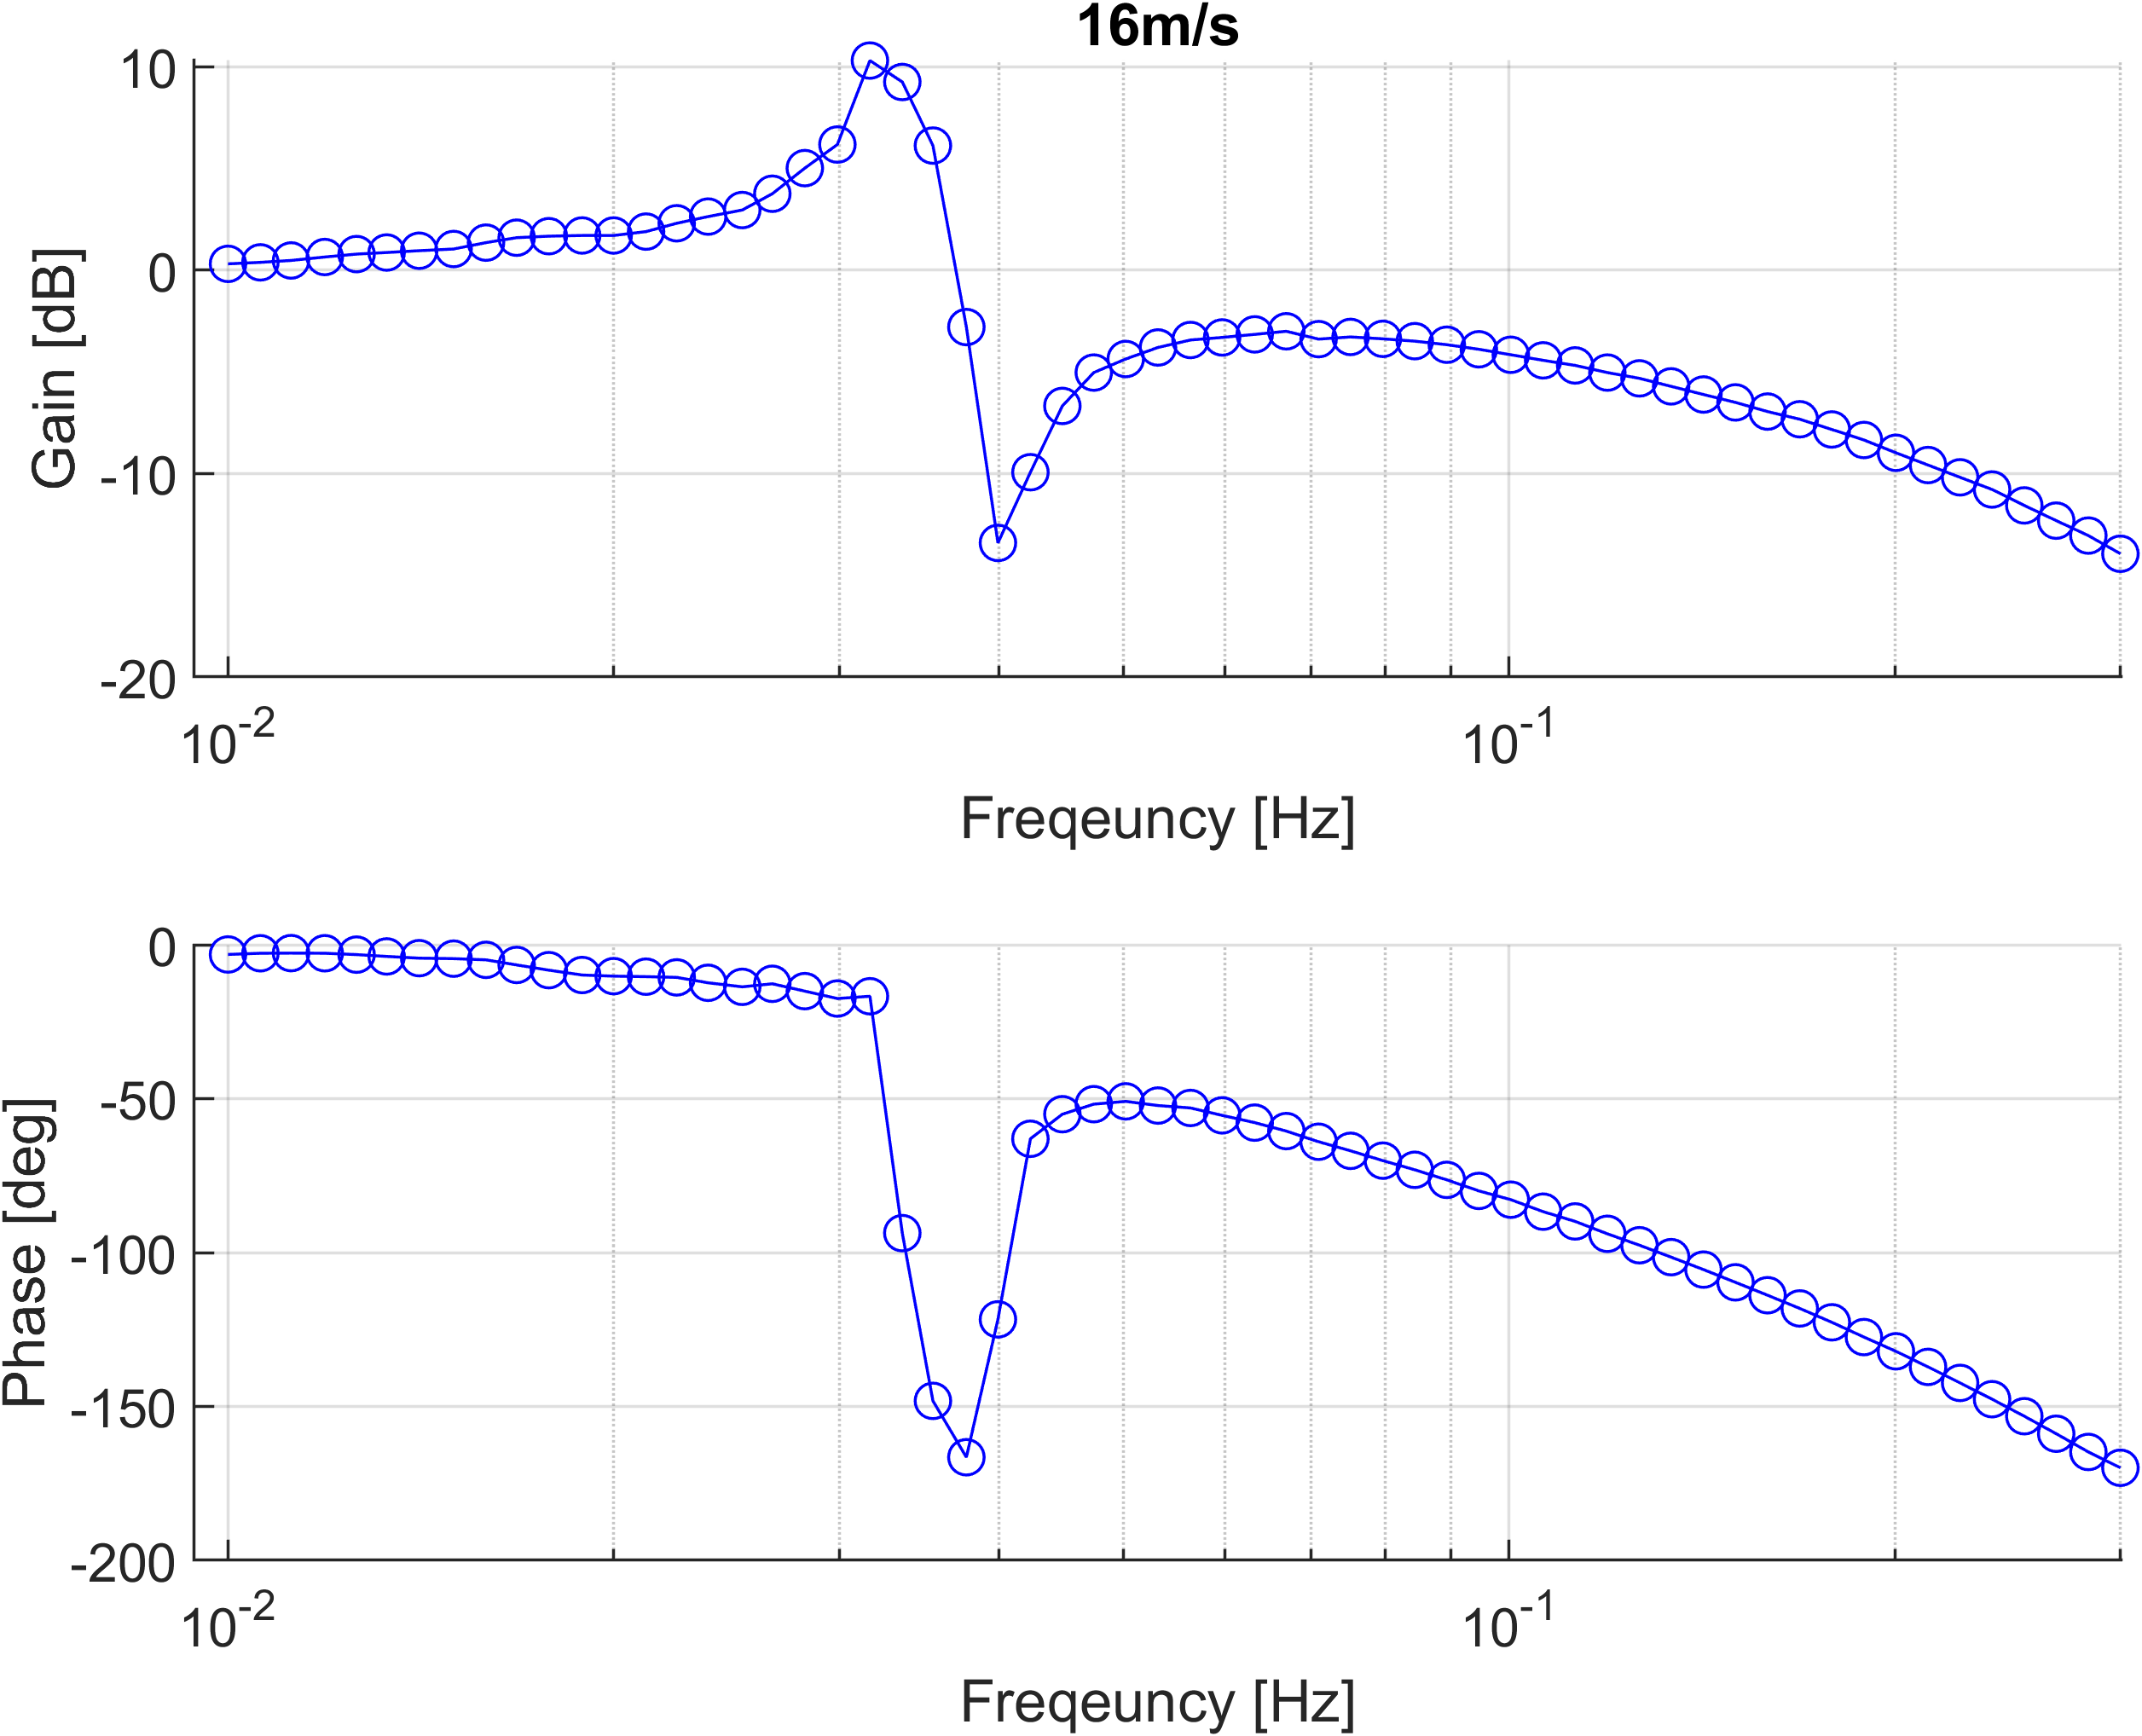
\includegraphics[width=.49\textwidth]{Graphics/TestResults/foreaftFitting/sysid_wRef-w_16ms.png}
		\label{fig:app_sysid_wref-w_16}}
	\hfil
	\subfloat[Linear model response]{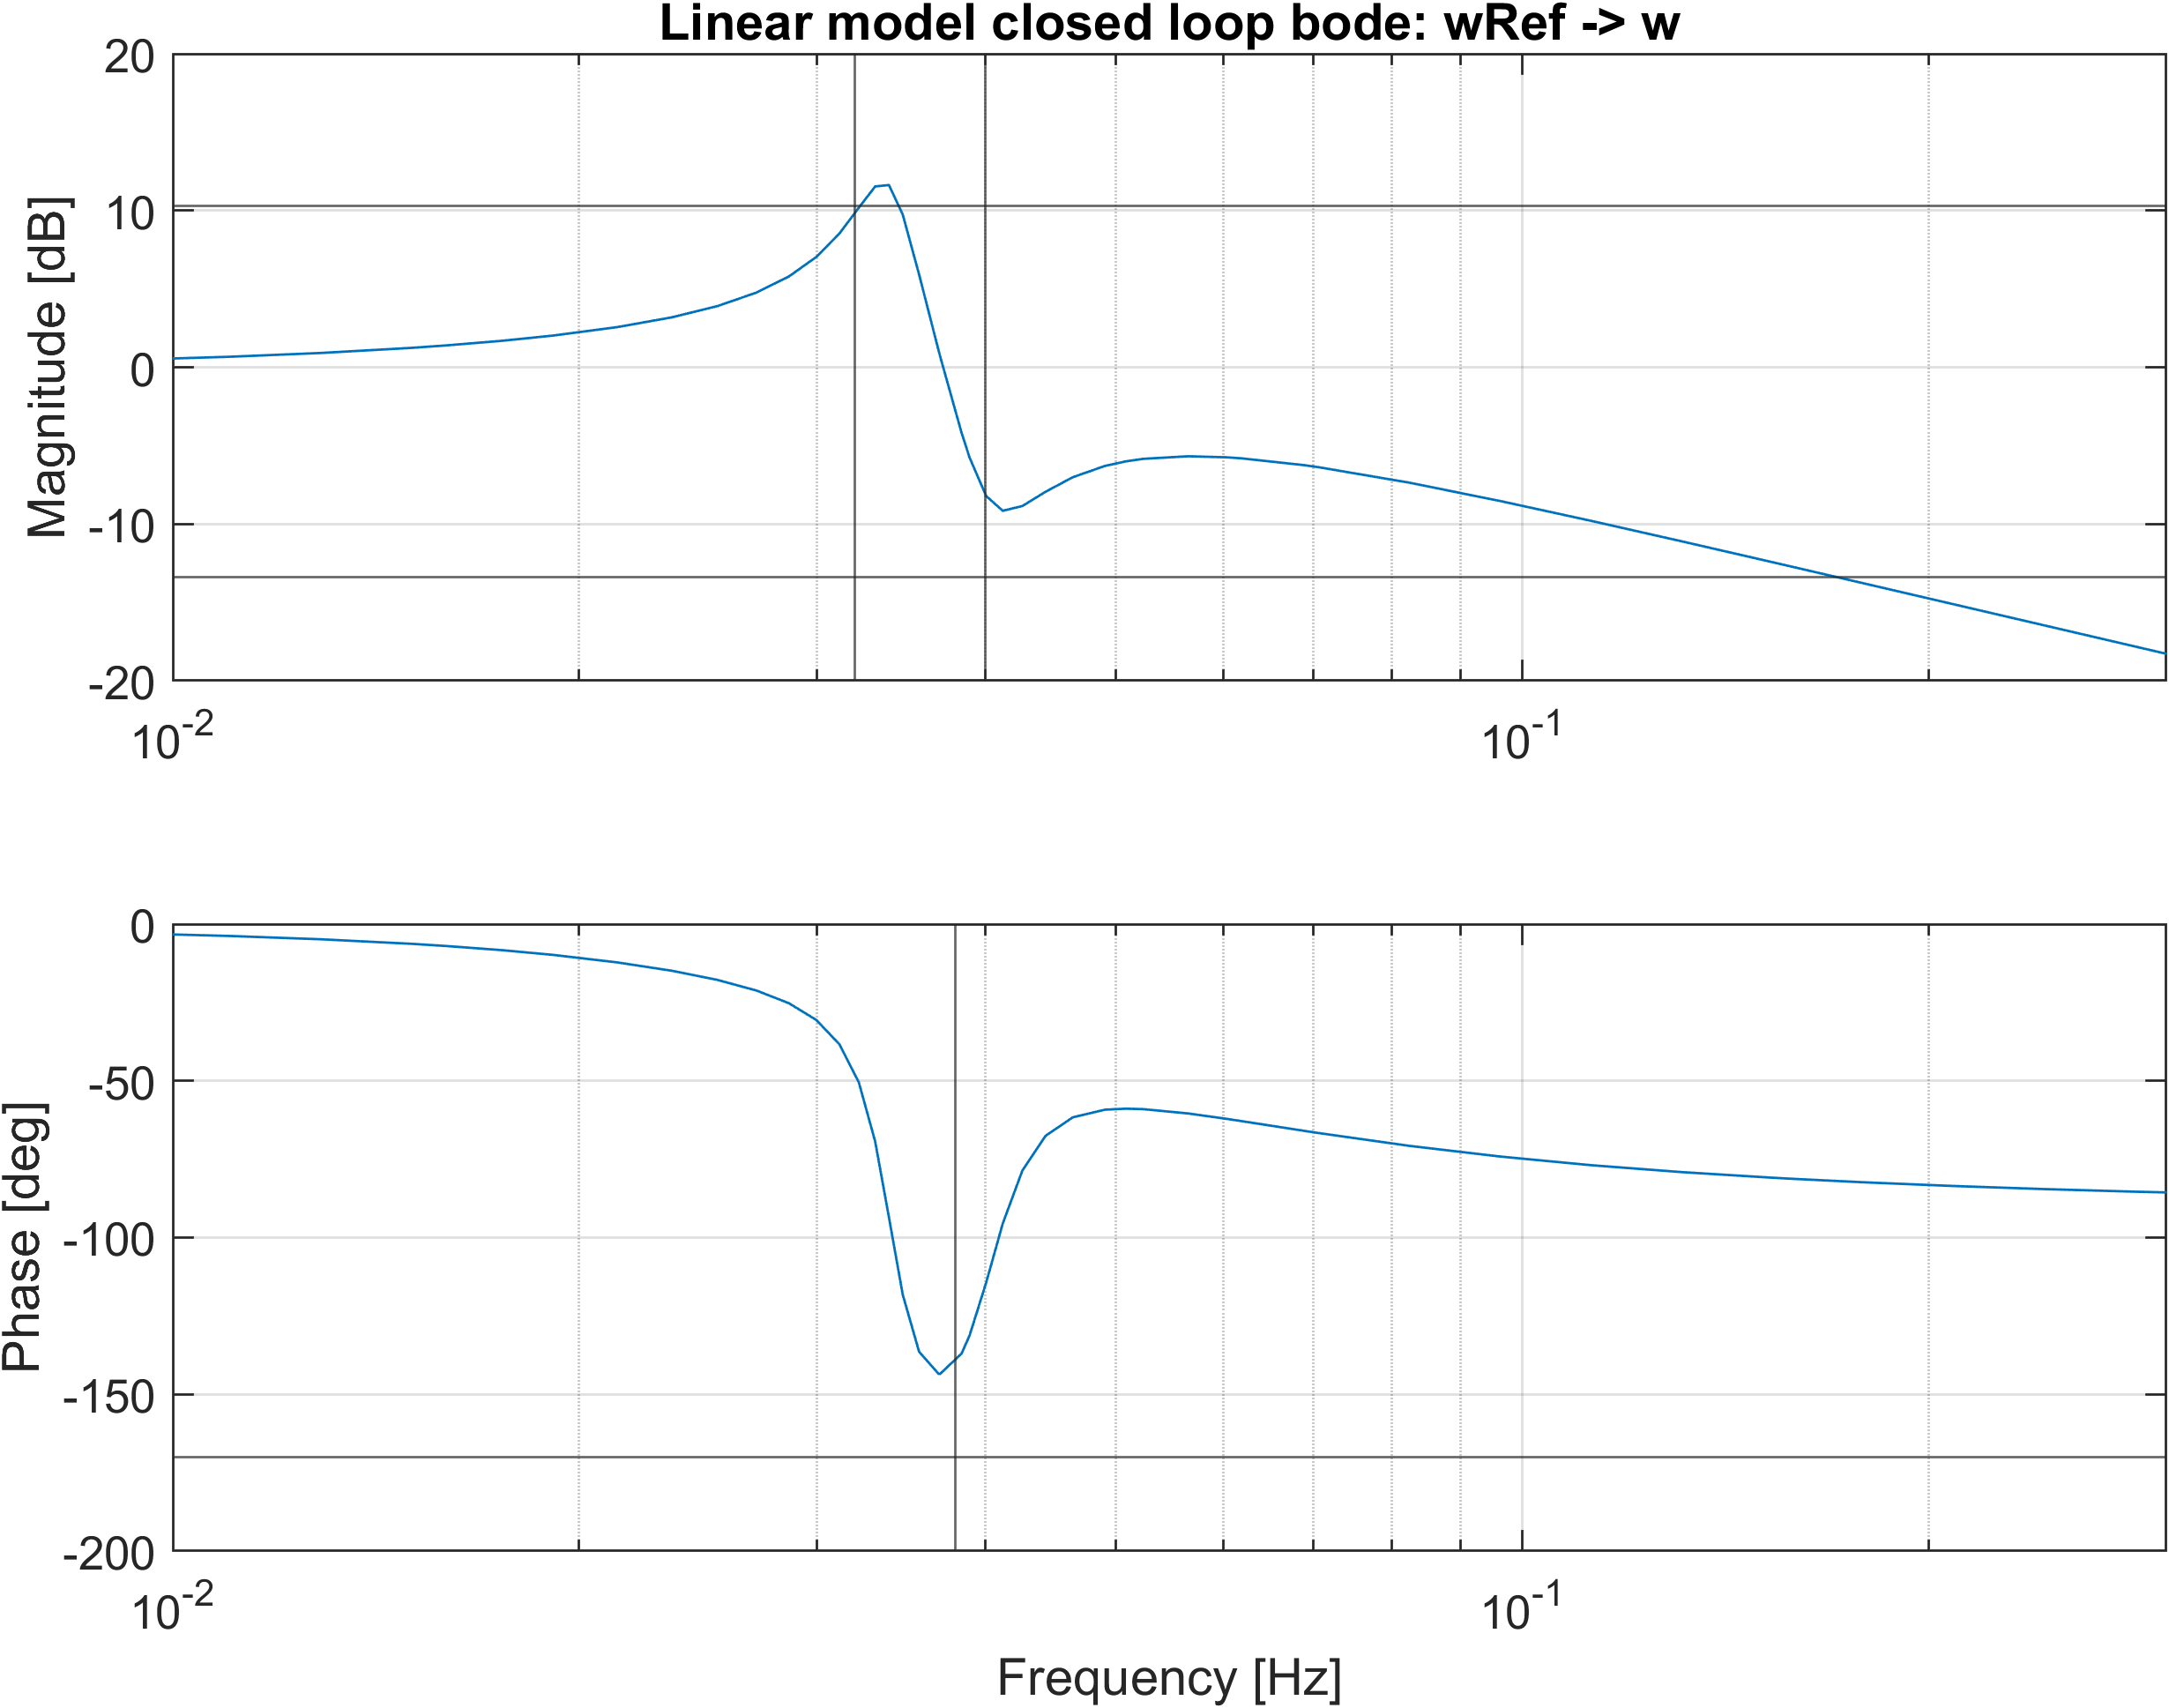
\includegraphics[width=.49\textwidth]{Graphics/TestResults/foreaftFitting/wtLin_wRef-w_16ms.png}
		\label{fig:app_wtlin_wref-w_16}}
	
	\caption{generator speed reference to generator speed fitting with operating point at 16 m/s; \textbf{(a)} VTS bode plot; \textbf{(b)} Linear model bode plot. Black lines are placed in the magnitude plot to indicate the peaks and valleys around the eigenfrequency and in the phase plot at the valley from (a).}
	\label{fig:app_wref-w_16}
\end{figure*}



\begin{figure*}[ht]
	\centering
	
	\subfloat[VTS frequency response]
	{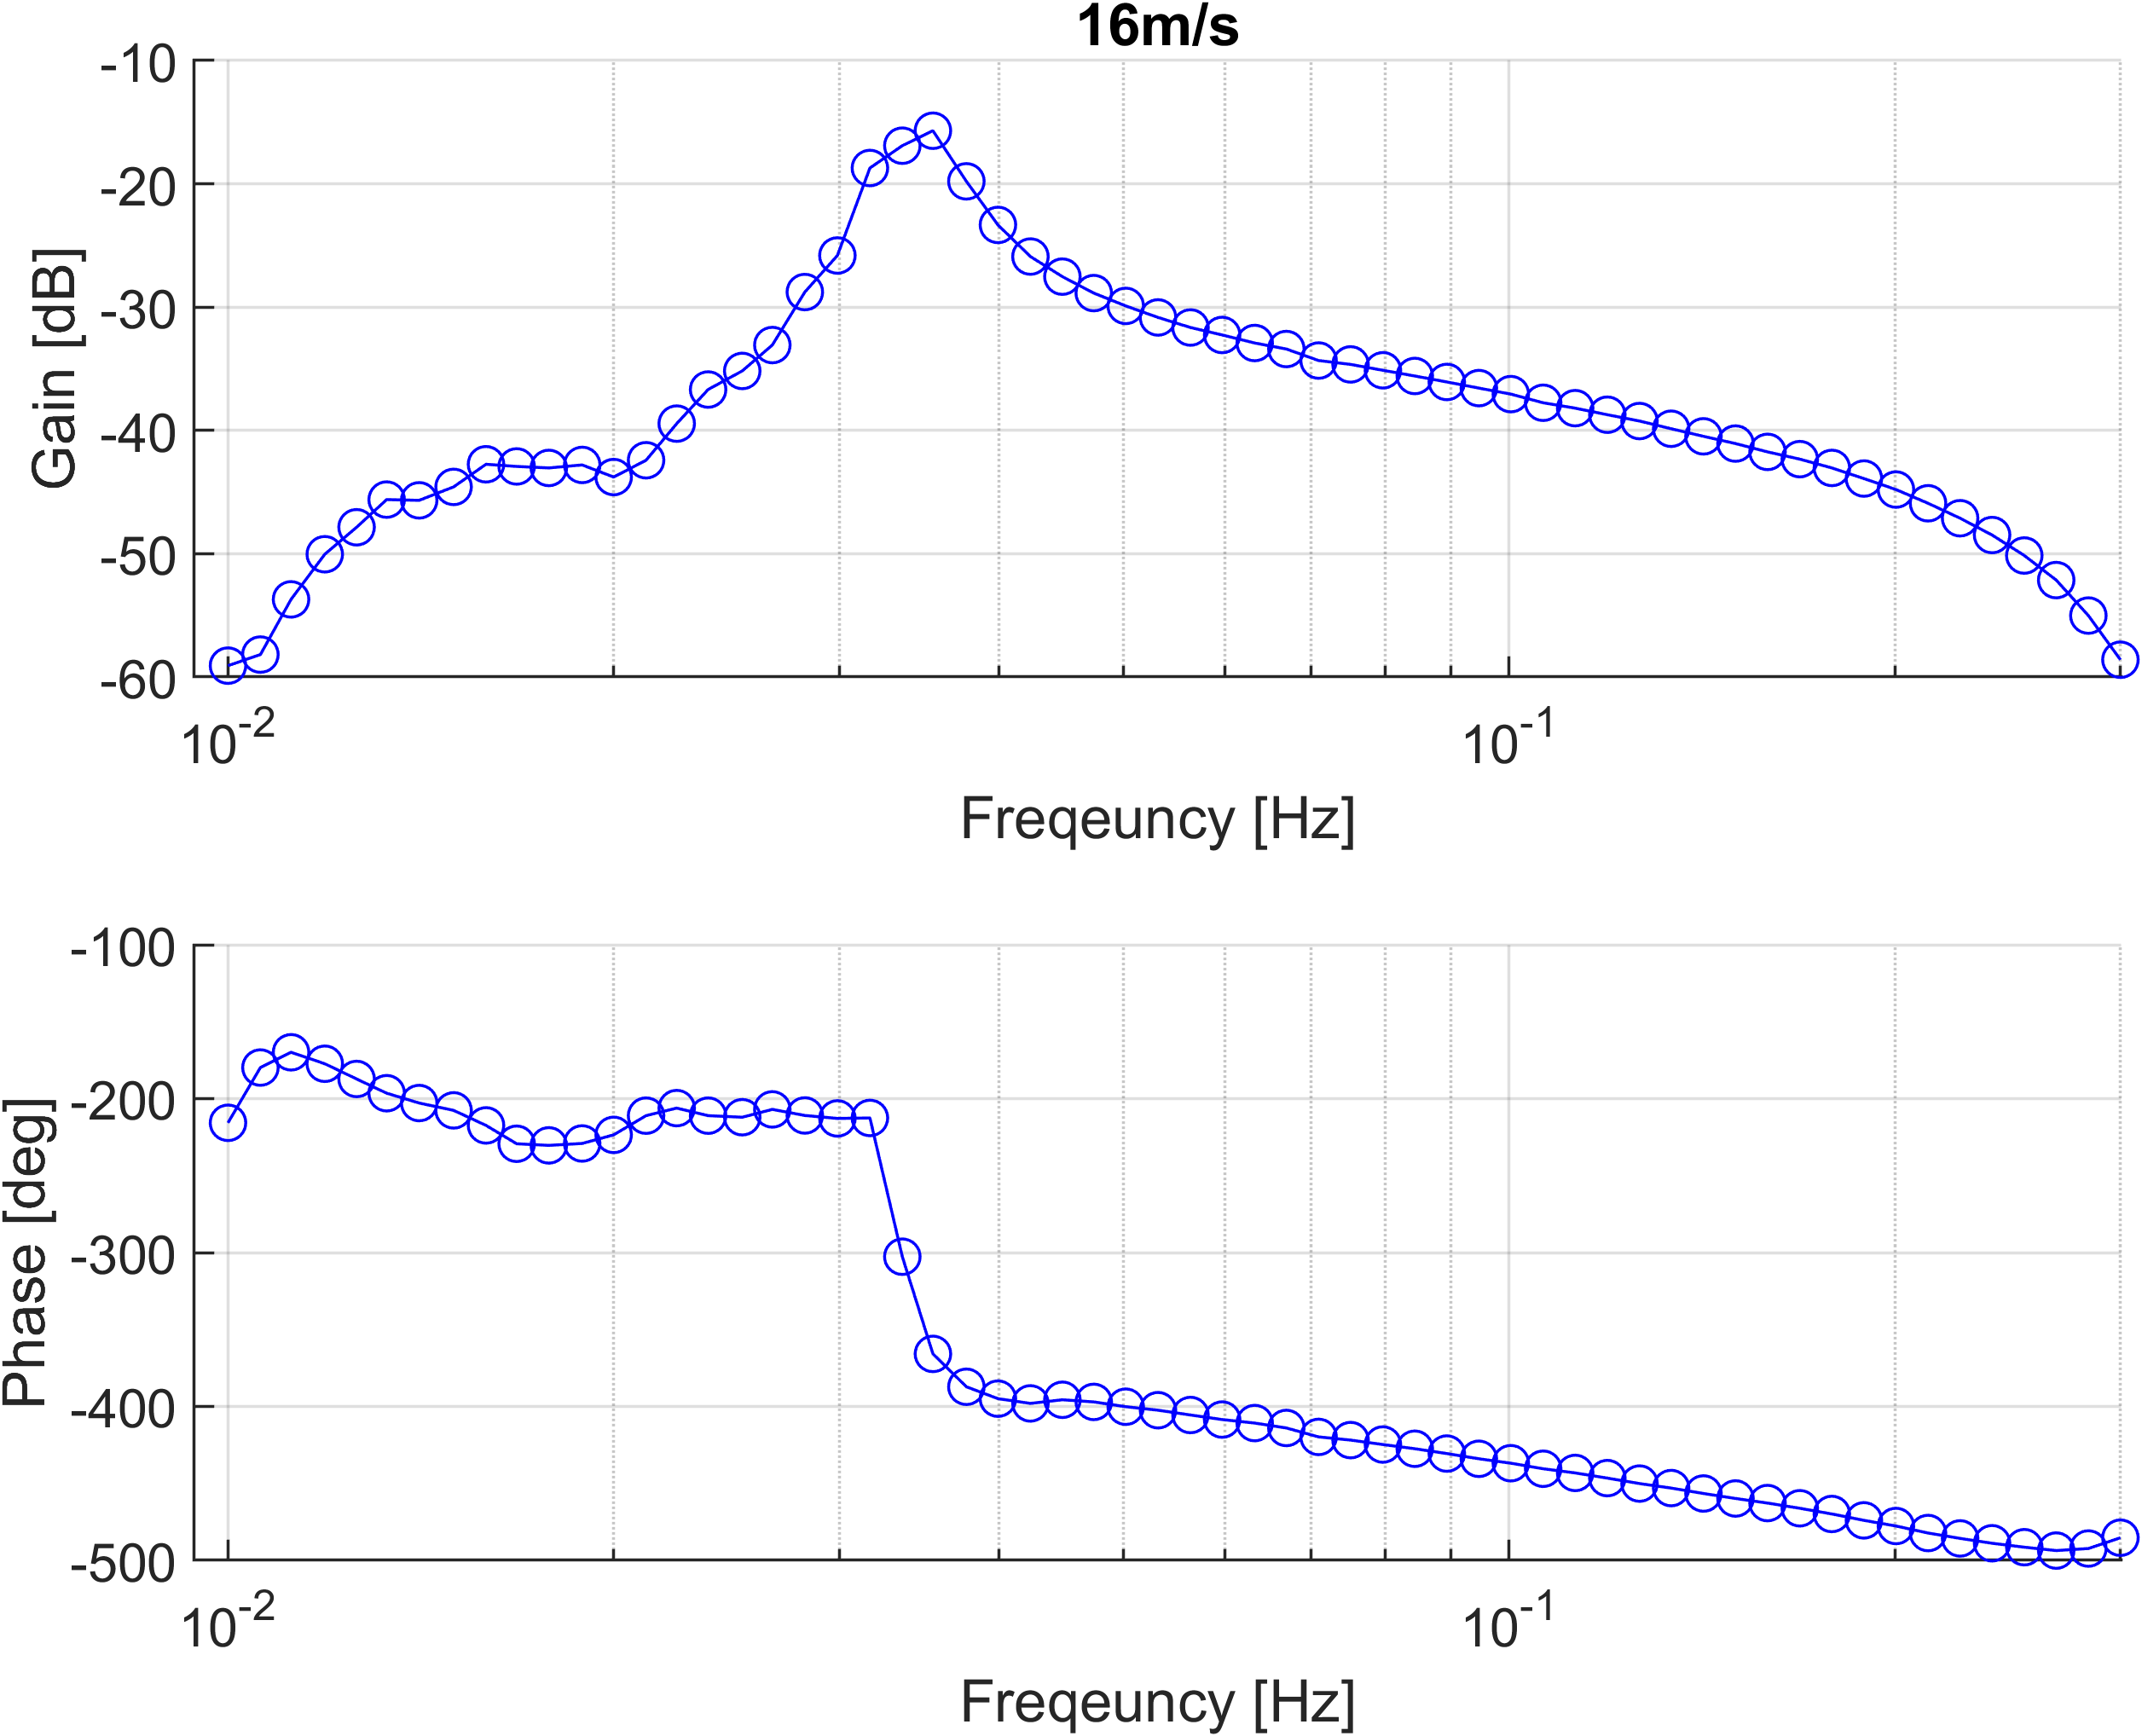
\includegraphics[width=.49\textwidth]{Graphics/TestResults/foreaftFitting/sysid_wRef-vy_16ms.png}%
			\label{fig:app_sysid_wref-vy_16}}
	\hfil
	\subfloat[Linear model response]
	{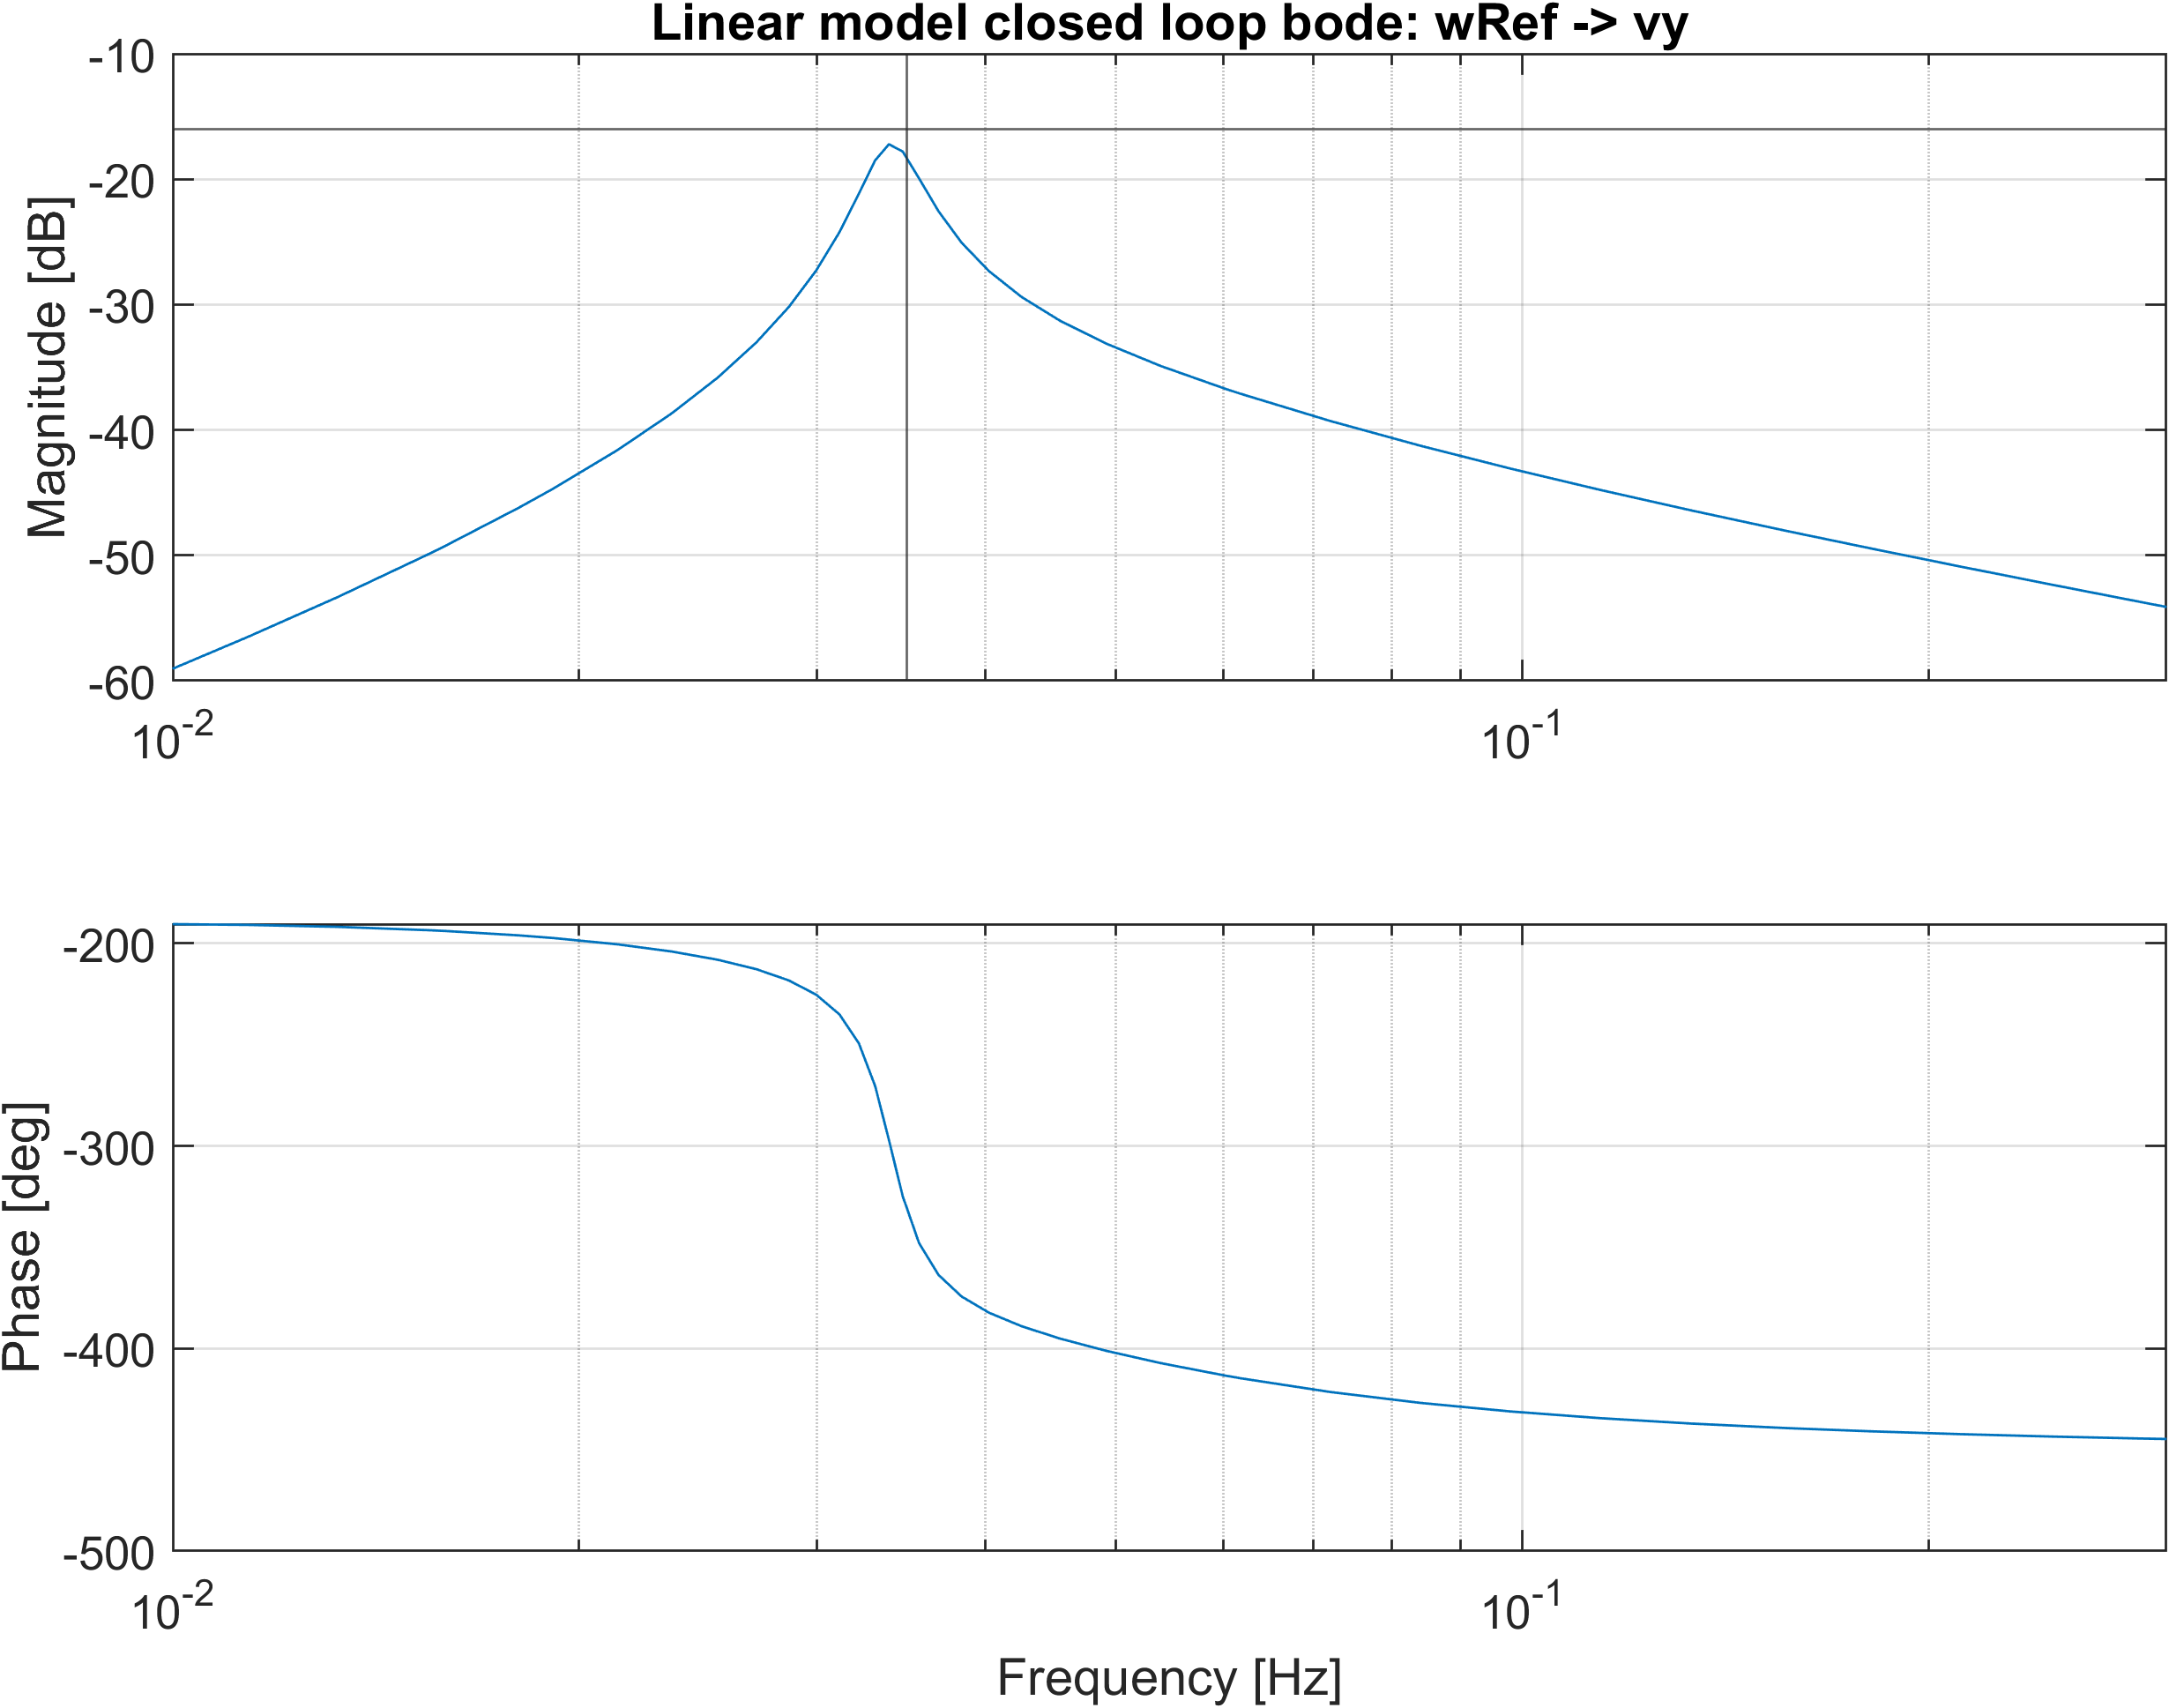
\includegraphics[width=.50\textwidth]{Graphics/TestResults/foreaftFitting/wtLin_wRef-vy_16ms.png}%
			\label{fig:app_wtlin_wref-vy_16}}
	
	\caption{generator speed reference to fore-aft surge velocity fitting with operating point at 16 m/s; \textbf{(a)} VTS bode plot; \textbf{(b)} Linear model bode plot. Black lines are placed in the magnitude plot to indicate position of magnitude peak from (a).}
	\label{fig:app_wref-vy_16}
\end{figure*}


\begin{figure*}[ht]
	\centering
	
	\subfloat[VTS frequency response]{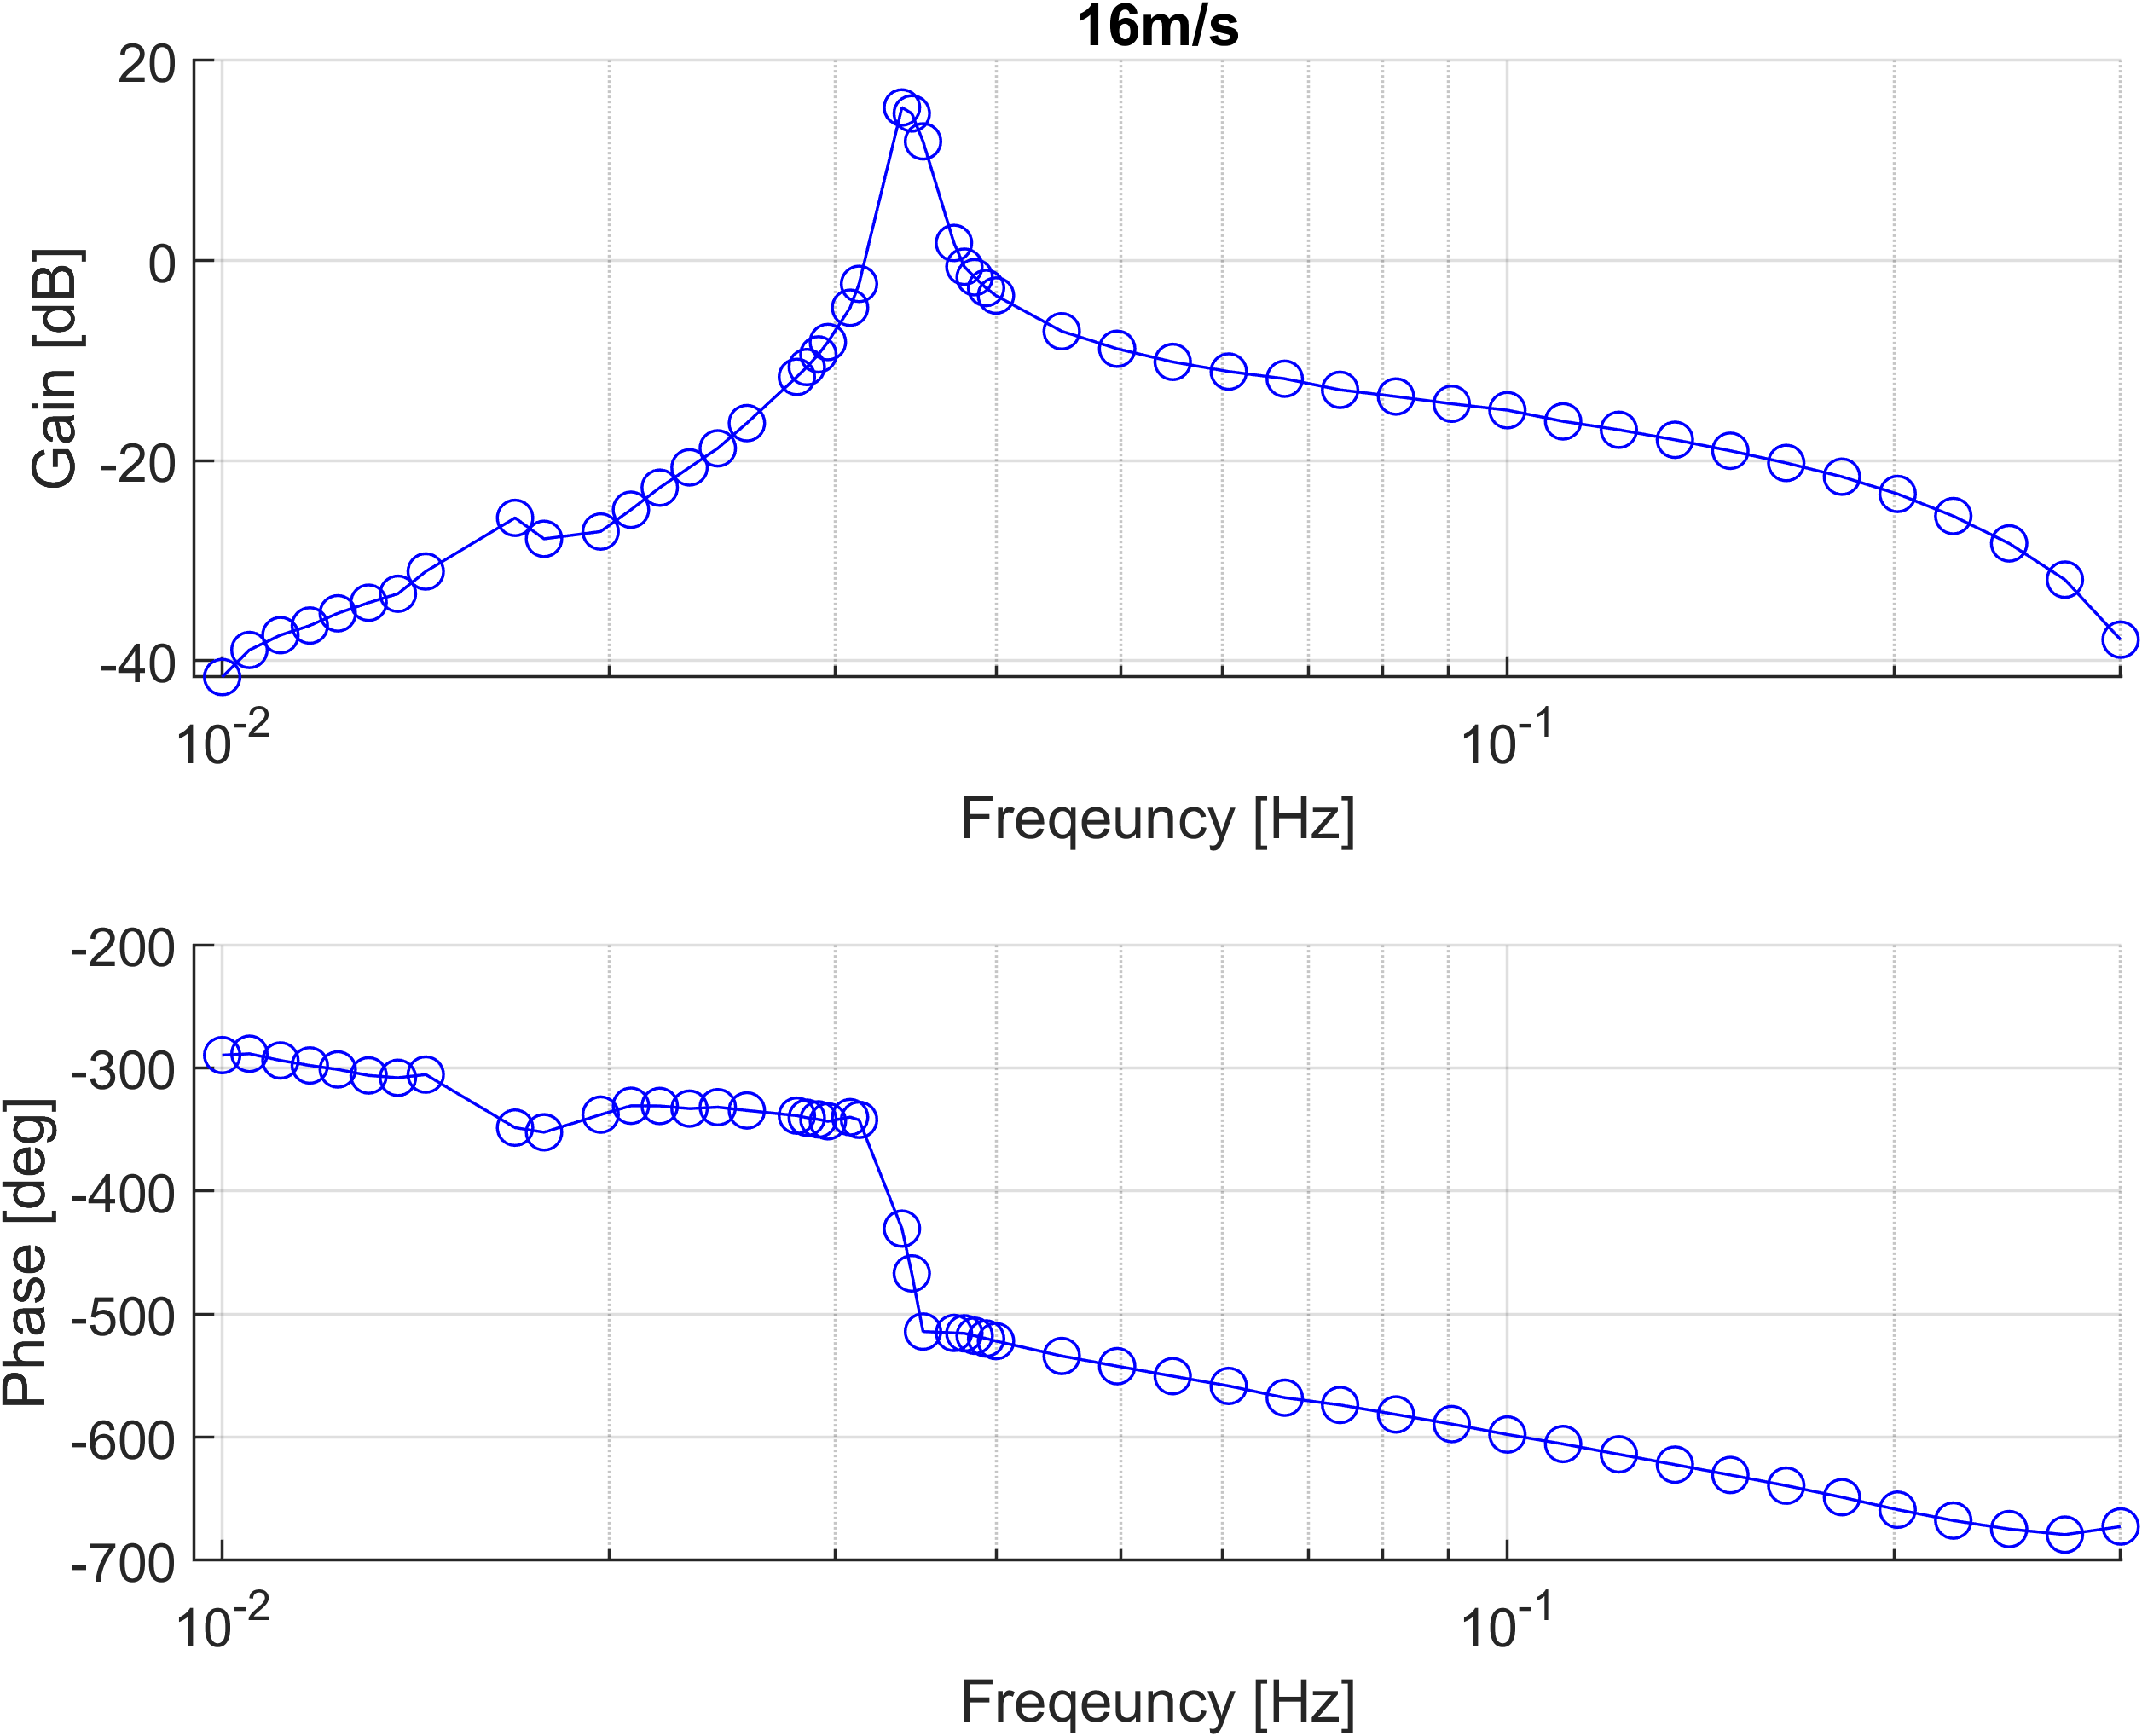
\includegraphics[width=.49\textwidth]{Graphics/TestResults/foreaftFitting/sysid_thSine-vy_16ms.png}
		\label{fig:app_sysid_thSine-vy_16}}
	\hfil
	\subfloat[Linear model response]{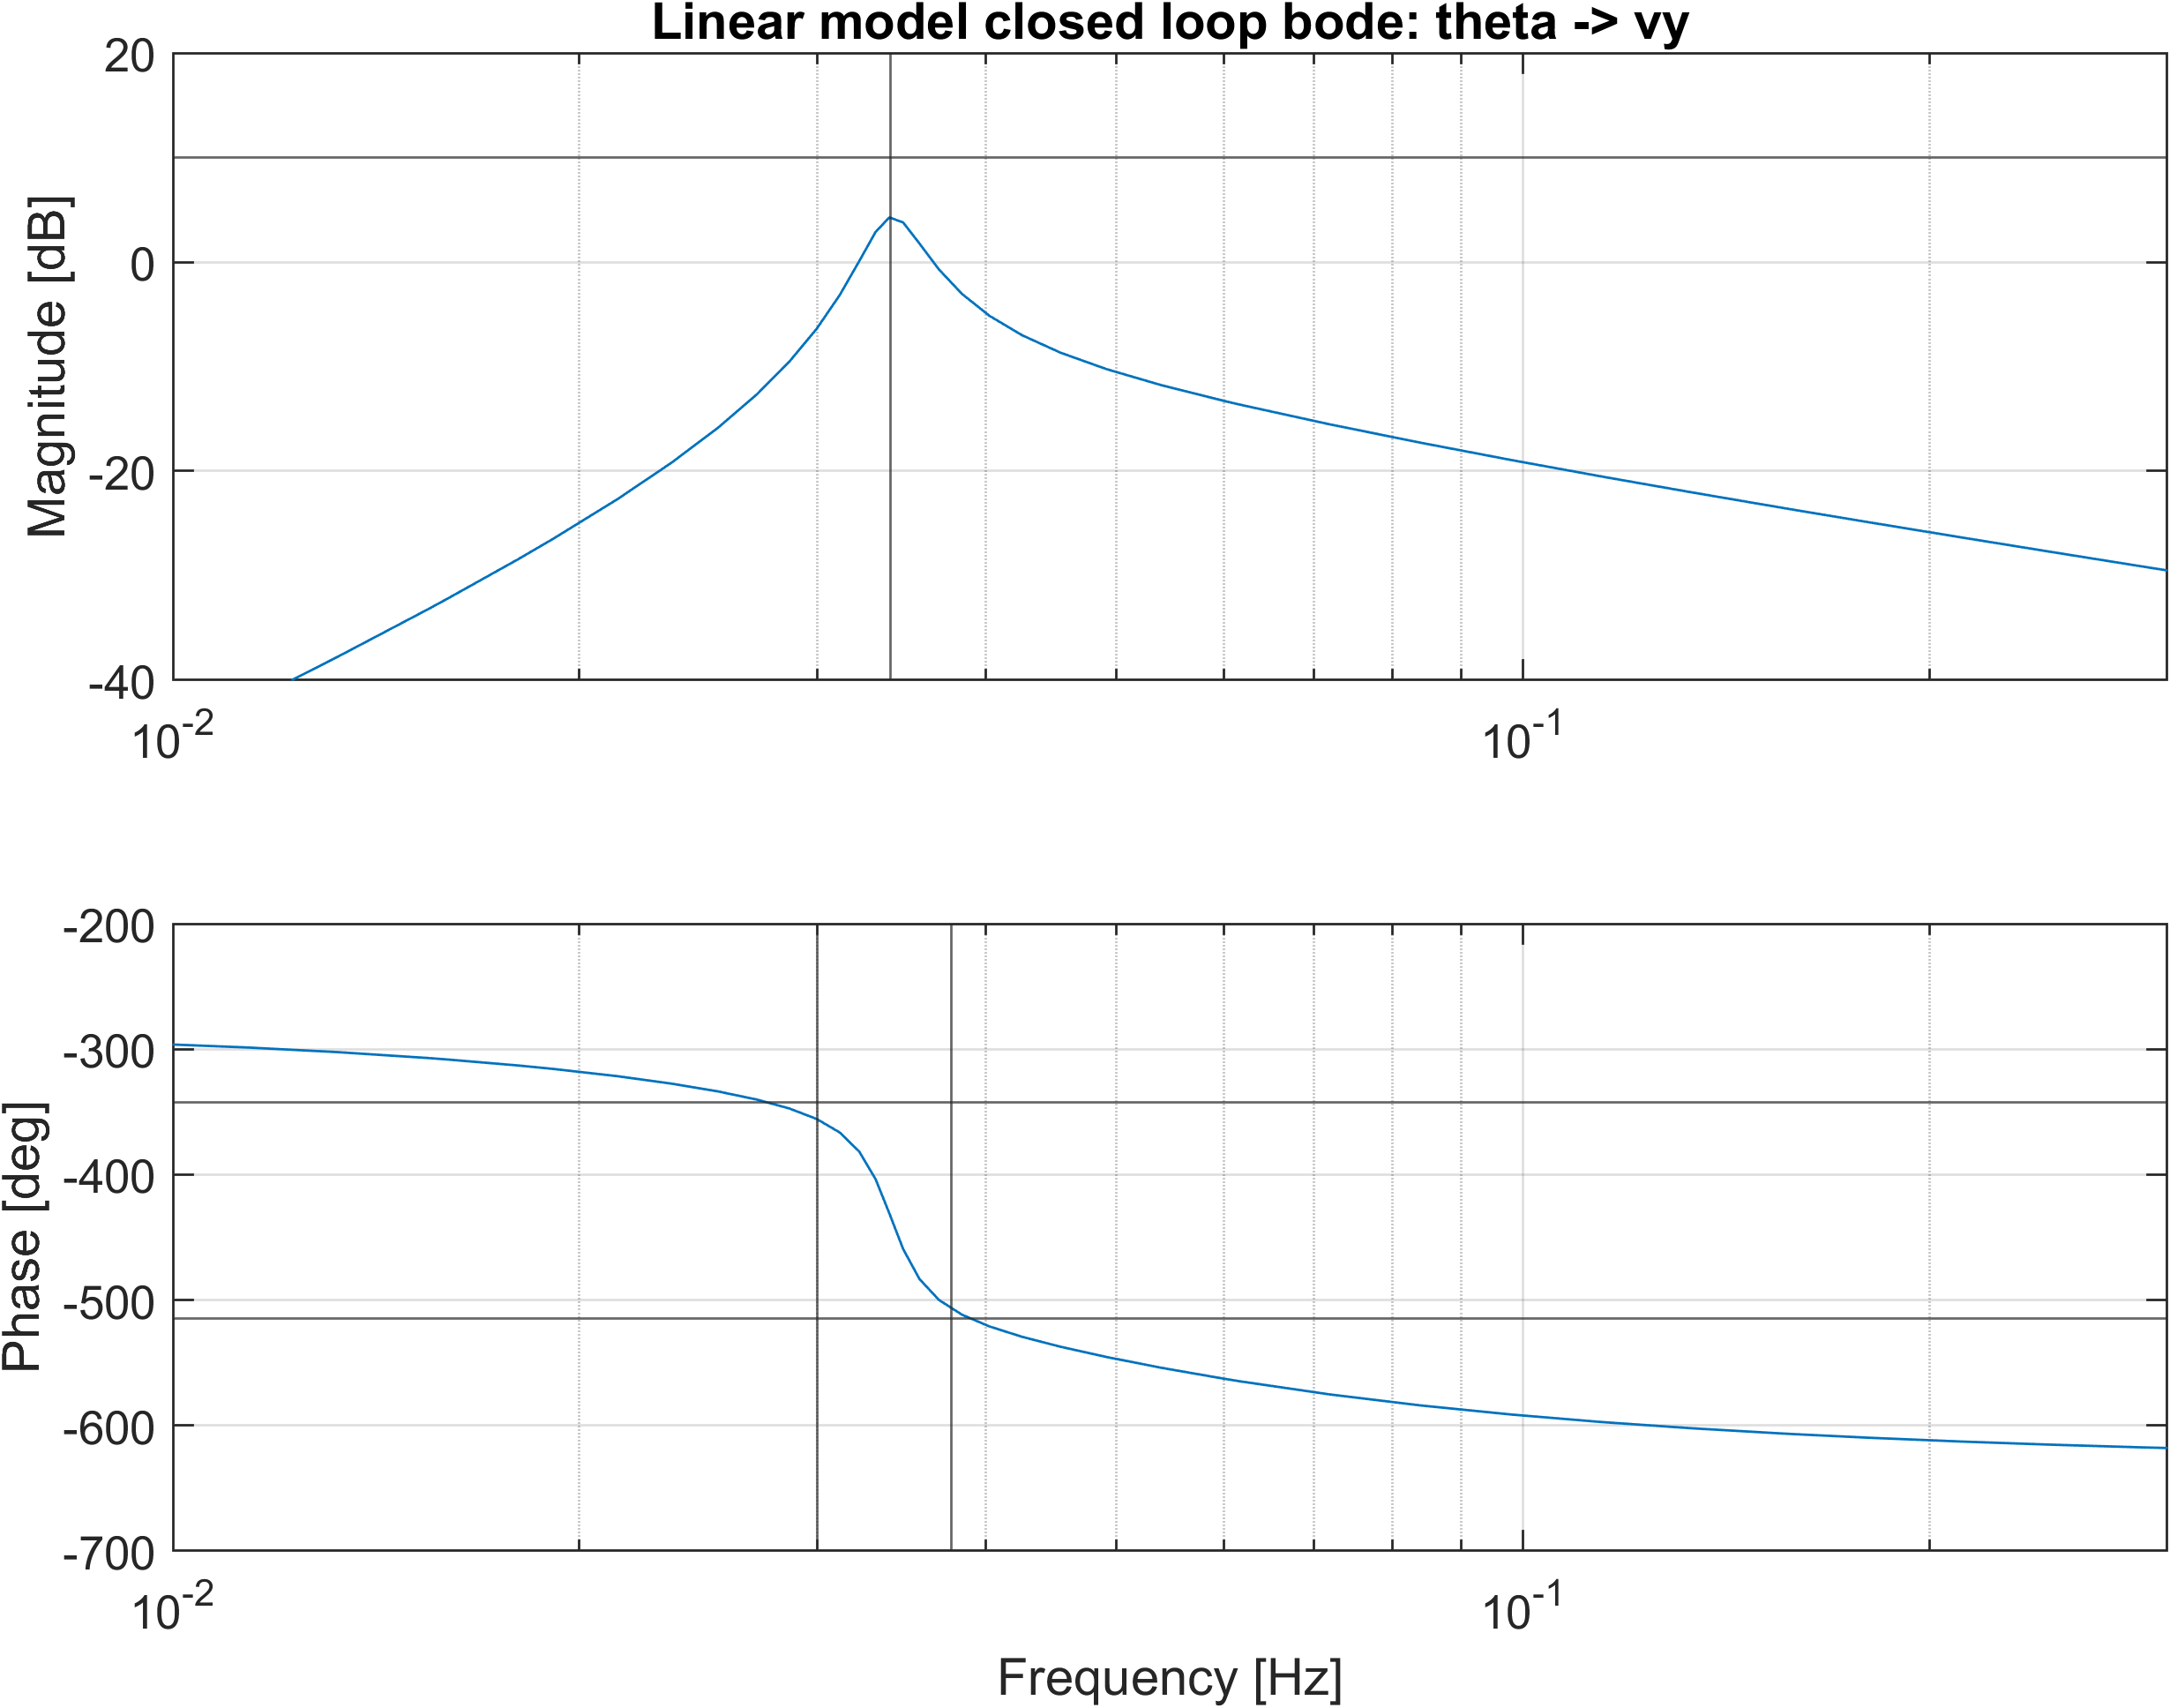
\includegraphics[width=.49\textwidth]{Graphics/TestResults/foreaftFitting/wtLin_th-vy_16ms.png}
		\label{fig:app_wtLin_th-vy_16}}
	
	\caption{pitch reference to fore-aft surge velocity fitting with operating point at 16 m/s; \textbf{(a)} VTS bode plot; \textbf{(b)} Linear model bode plot. Black lines are positioned in the magnitude plot to indicate the location of the peak of the VTS bode plot magnitude in (a). Black lines also indicate the position of the beginning and end of the large phase shift around the eigenfrequency from (a).}
	\label{fig:app_th-vy_16}
\end{figure*}



% Template
%\begin{figure*}[ht]
%	\centering
%	
%	\subfloat[VTS frequency response]
%	{\includegraphics[width=.49\textwidth]{Graphics/}%
%		\label{fig:app_sysid_}}
%	\hfil
%	\subfloat[Linear model response]
%	{\includegraphics[width=.50\textwidth]{Graphics/}%
%		\label{fig:app_wtlin_}}
%	
%	\caption{General_text; \textbf{(a)} a_text; \textbf{(b)} b_text.}
%	\label{fig:app_full}
%\end{figure*}


\subsection{Test: Linear model} \label{sec:app_test_lin}
The purpose of this test is to show and discuss the performance results of the LQI controller derived in \cref{sec:ctrl-design} on the linear model derived in \cref{sec:linear_model}. The controller is benchmarked against the original FLC controller with regards to both rotor speed control and fore-aft movement dampening capability. Prior to the test the LQI controller has been tuned such that a satisfactory performance was achieved in VTS.

It is expected that the LQI controller will perform much better in damping the fore-aft movement than the original FLC PI controller with no FATD. Test results are shown for both frequency and time domain.

% It is also expected to perform better in generator speed control despite the fact that the original FLC controller has been tuned to achieve the best possible generator speed tracking performance. The reason for this prediction might be less obvious. The reason is that the LQI controller has been tuned on the simple linear model and not in VTS like the FLC PI controller. Thus potential unforeseen consequences of having an aggressive controller in a more realistic environment are not discovered until it is tested in VTS.

\subsubsection{Test framework}
Matlab is used to makedf bode plots and Matlab Simulink is used to run time simulations. The Matlab \textit{connect()} function is utilized with component models defined on a specific form to gain transfer functions or state space systems from one or more inputs to one or more outputs. From these the \textit{bode()} Matlab function is used to make bode plots. 

Time simulations are made with the FLC PI and LQI controlled linear models from the $ A $, $ B $ and $ C $ system matrices and controller gains $ K $. In \cref{fig:app_simulink_setup2} the Simulink simulation setup is seen. Two systems are observed with the top one containing the original FLC PI controller without FATD enabled and the bottom one being the one with the designed LQI controller. While not directly apparent because of the missing state feedback, the top system is a closed loop system with the controller gain $ K $ contained in the $ A $ and $ B $ matrix. The reason for this is simply that the FLC component described in \cref{sec:comp_flc} is defined as a generic component model and conveniently combined with the Matlab \textit{connect()} function to yield a full closed-loop system.

From the left the free wind disturbance deviation from the OP is observed entering both systems. The wind data is extracted from VTS simulations and thus mimic the wind turbulence realistically. The simulation is run for a total of 1000 seconds and the states are initialized at the OP except for the tower top position $ p_y $ which is initialized with a deviation of 5 m to provoke a response from both systems.
\begin{figure}[ht]
	\centering
	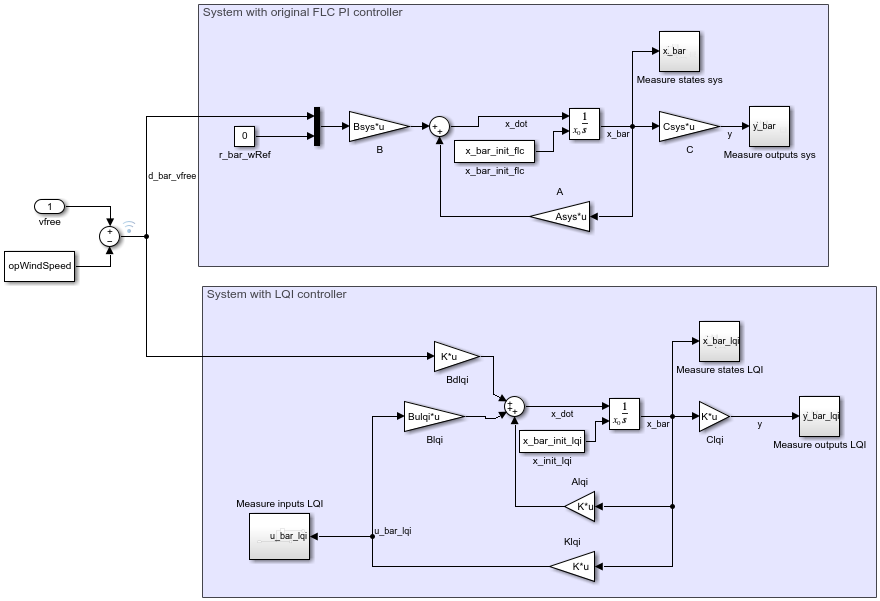
\includegraphics[width=0.95\linewidth]{Graphics/TestResults/linearModPerf/simulink_setup2.png}
	\caption{The Matlab Simulink setup. The free wind speed is observed entering the system from the left.}
	\label{fig:app_simulink_setup2}
\end{figure}


\subsubsection{Frequency Domain}
In figure \cref{fig:app_script_vfreeTovy} the frequency response from the free wind disturbance $ v_{free} $ to the fore-aft tower top velocity $ v_y $ is seen. Both the FLC PI system and LQI system are plotted for comparison. It is observed that the LQI controller yields much greater dampening of the eigenfrequency than the FLC PI controller.
\begin{figure}[ht]
	\centering
	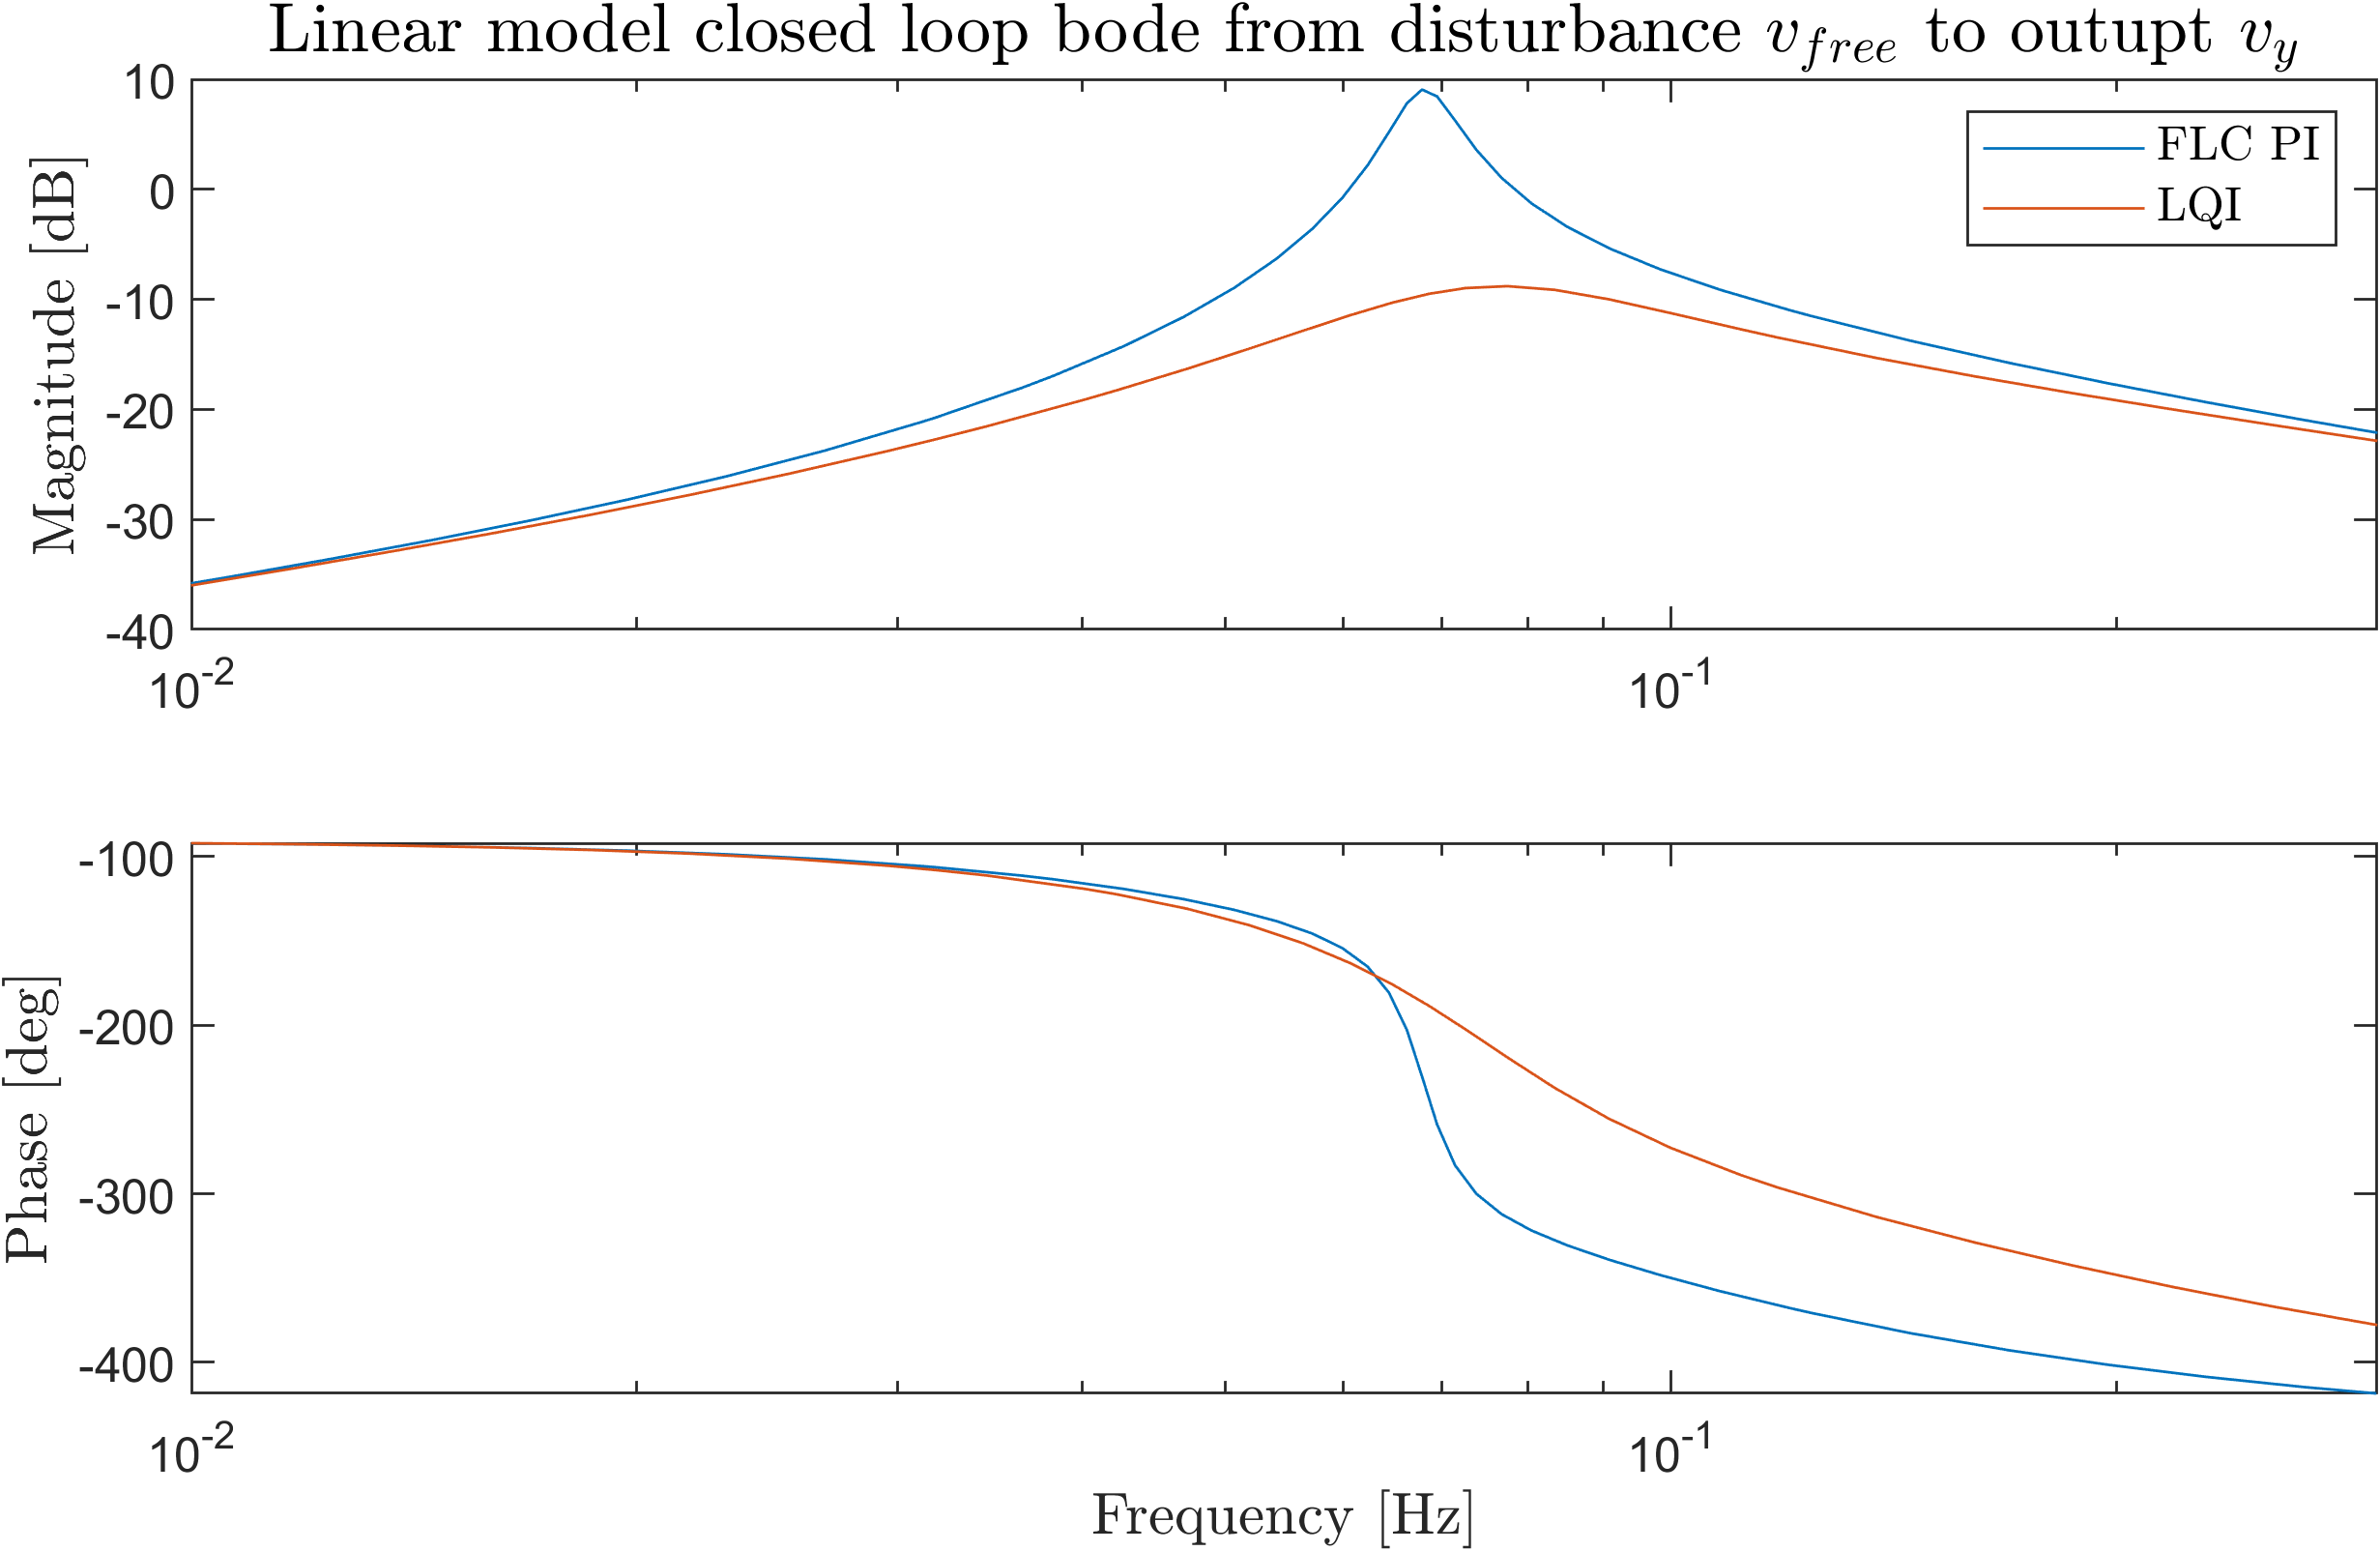
\includegraphics[width=0.7\linewidth]{Graphics/TestResults/linearModPerf/script_vfreeTovy.png}
	\caption{Frequency response from the free wind as observed by the rotor ($ v_{free} $) to the fore-aft velocity ($ v_y $) of the linear model with a comparison between the original FLC PI controller and the LQI controller.}
	\label{fig:app_script_vfreeTovy}
\end{figure}
In \cref{fig:app_script_vfreeTovy} where the frequency response from $ v_{free} $ to $ \Omega $ is plotted the same tendency is observed. The LQI controller furthermore dampens the magintude around 4-7 dB more than the FLC PI controller before the eigenfrequency around 0.035 Hz. It also dampens the magnitude more after the eigenfrequency but decreasingly for higher frequencies.
\begin{figure}[ht]
	\centering
	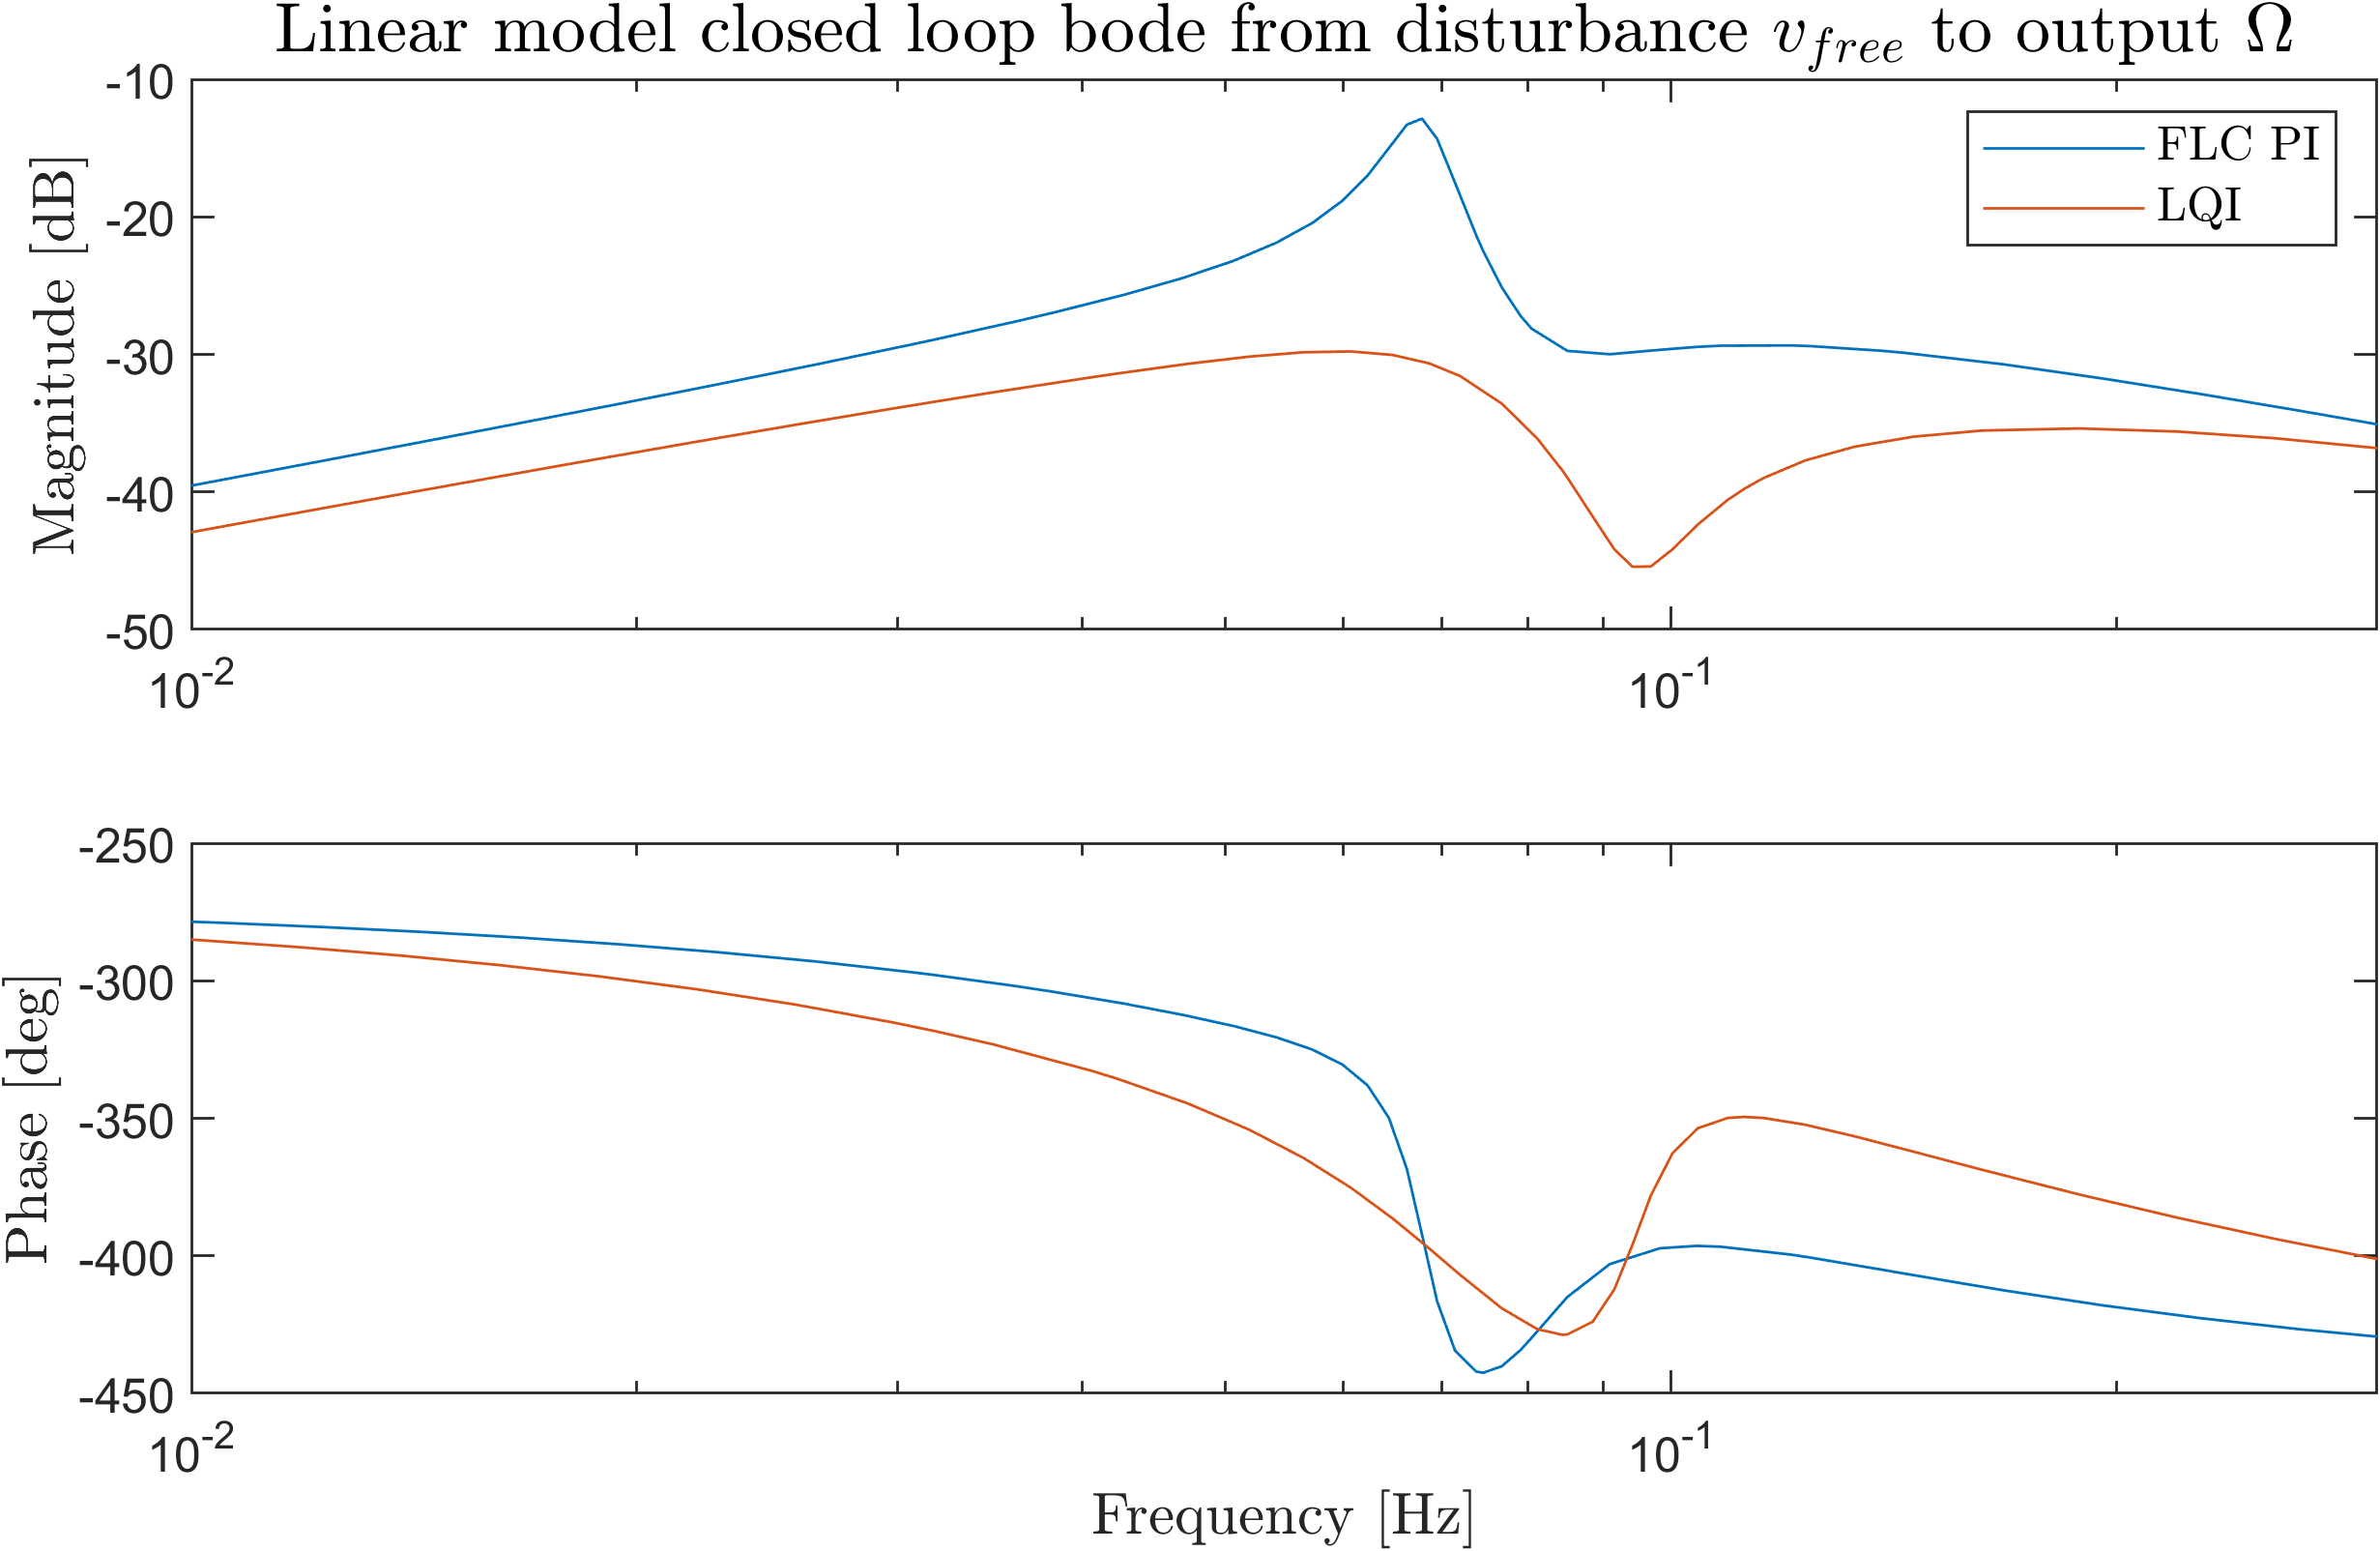
\includegraphics[width=0.7\linewidth]{Graphics/TestResults/linearModPerf/script_vfreeToW.png}
	\caption{Frequency response from the free wind as observed by the rotor ($ v_{free} $) to the rotor speed ($ \Omega $) of the linear model with a comparison between the original FLC PI controller and the LQI controller}
	\label{fig:app_script_vfreeToW}
\end{figure}
From the frequency responses it can be concluded that the LQI controller will perform better at both rotor speed tracking and fore-aft movement damping. 

\clearpage
\subsubsection{Time domain}
In \cref{fig:app_sim_11_W_py_vy_comp} the rotor speed, fore-aft position and fore-aft velocity is plotted. Both the FLC PI and LQI controlled systems are plotted for comparison. Both rotor speed tracking and fore-aft motion performance is vastly superior for the LQI controller. The poor rotor speed tracking performance of the FLC controller is expected because of its lack of consideration for the fore-aft motion.
\begin{figure}[ht]
	\centering
	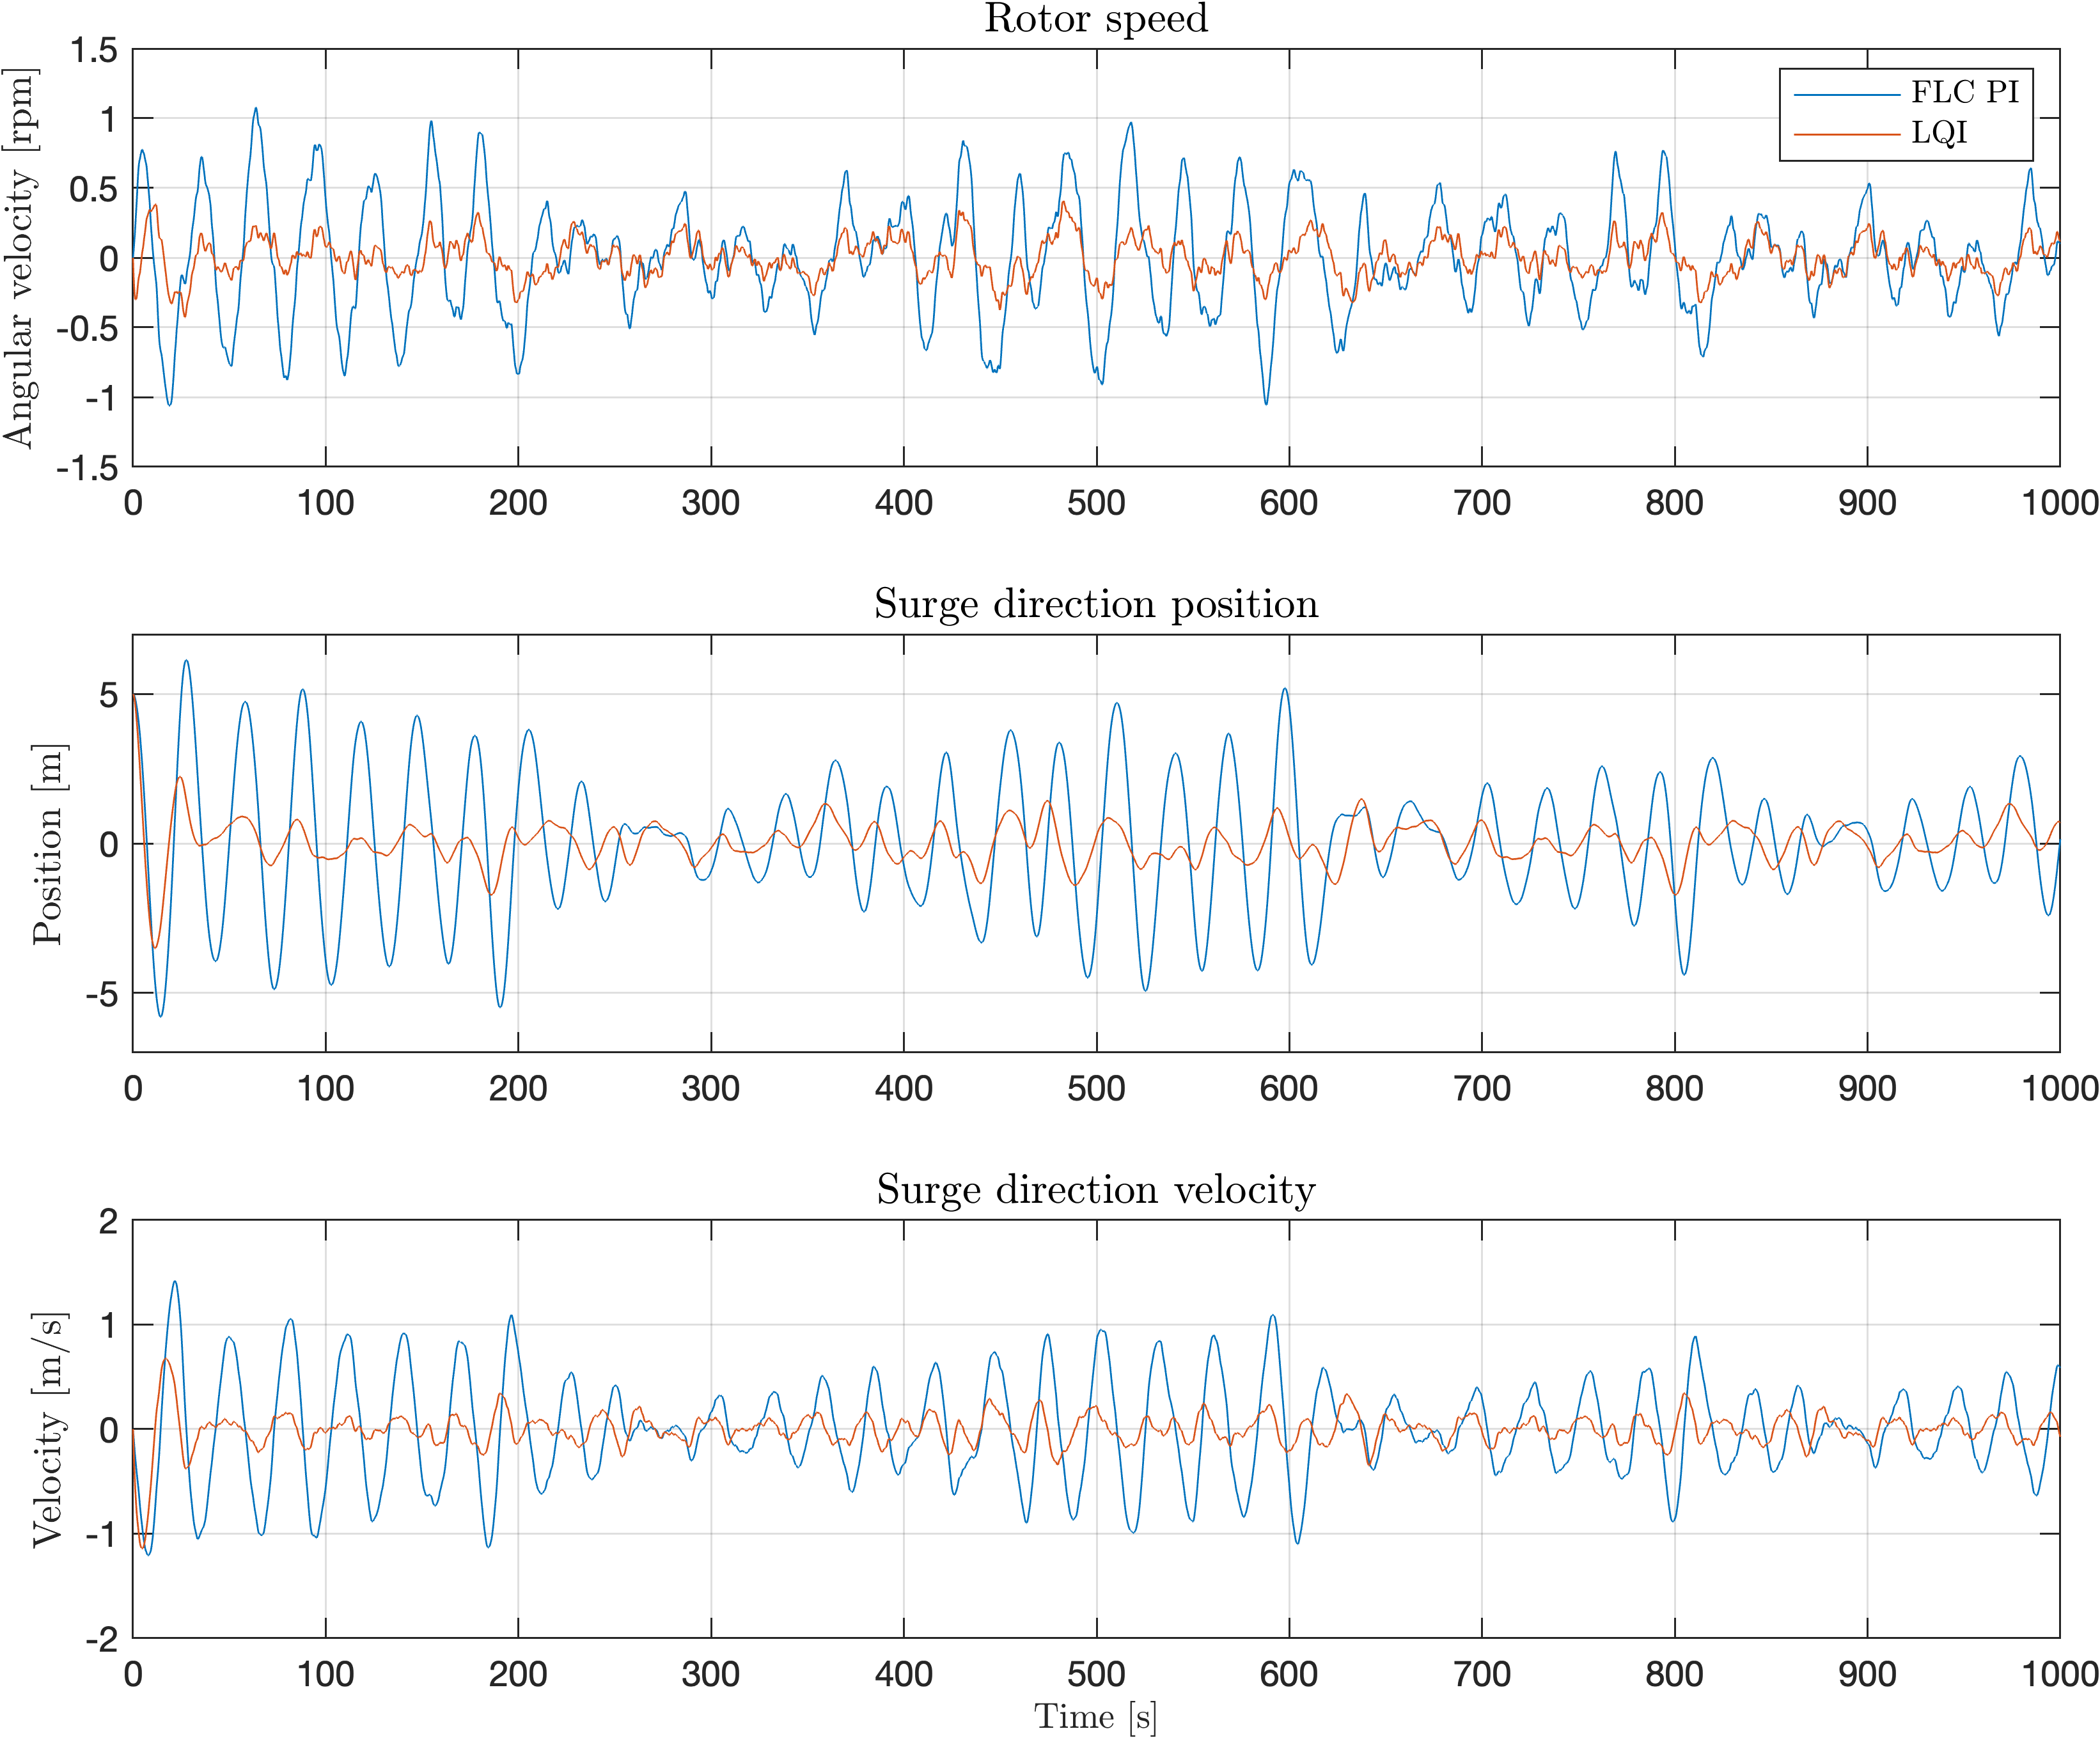
\includegraphics[width=0.7\linewidth]{Graphics/TestResults/linearModPerf/sim_11_W_py_vy_comp.png}
	\caption{Simulink simulation results. The 5 m deviation initialization of the tower top position is visible from the \textit{fore-aft position} at 0 s.}
	\label{fig:app_sim_11_W_py_vy_comp}
\end{figure}
\cref{fig:app_sim_12_W_py_vy_comp_zoom} shows a plot zoomed in at the start of the simulation. It is apparent that the LQI controller corrects for the fore-aft position deviation effectively in 30 to 40 seconds.
\begin{figure}[ht]
	\centering
	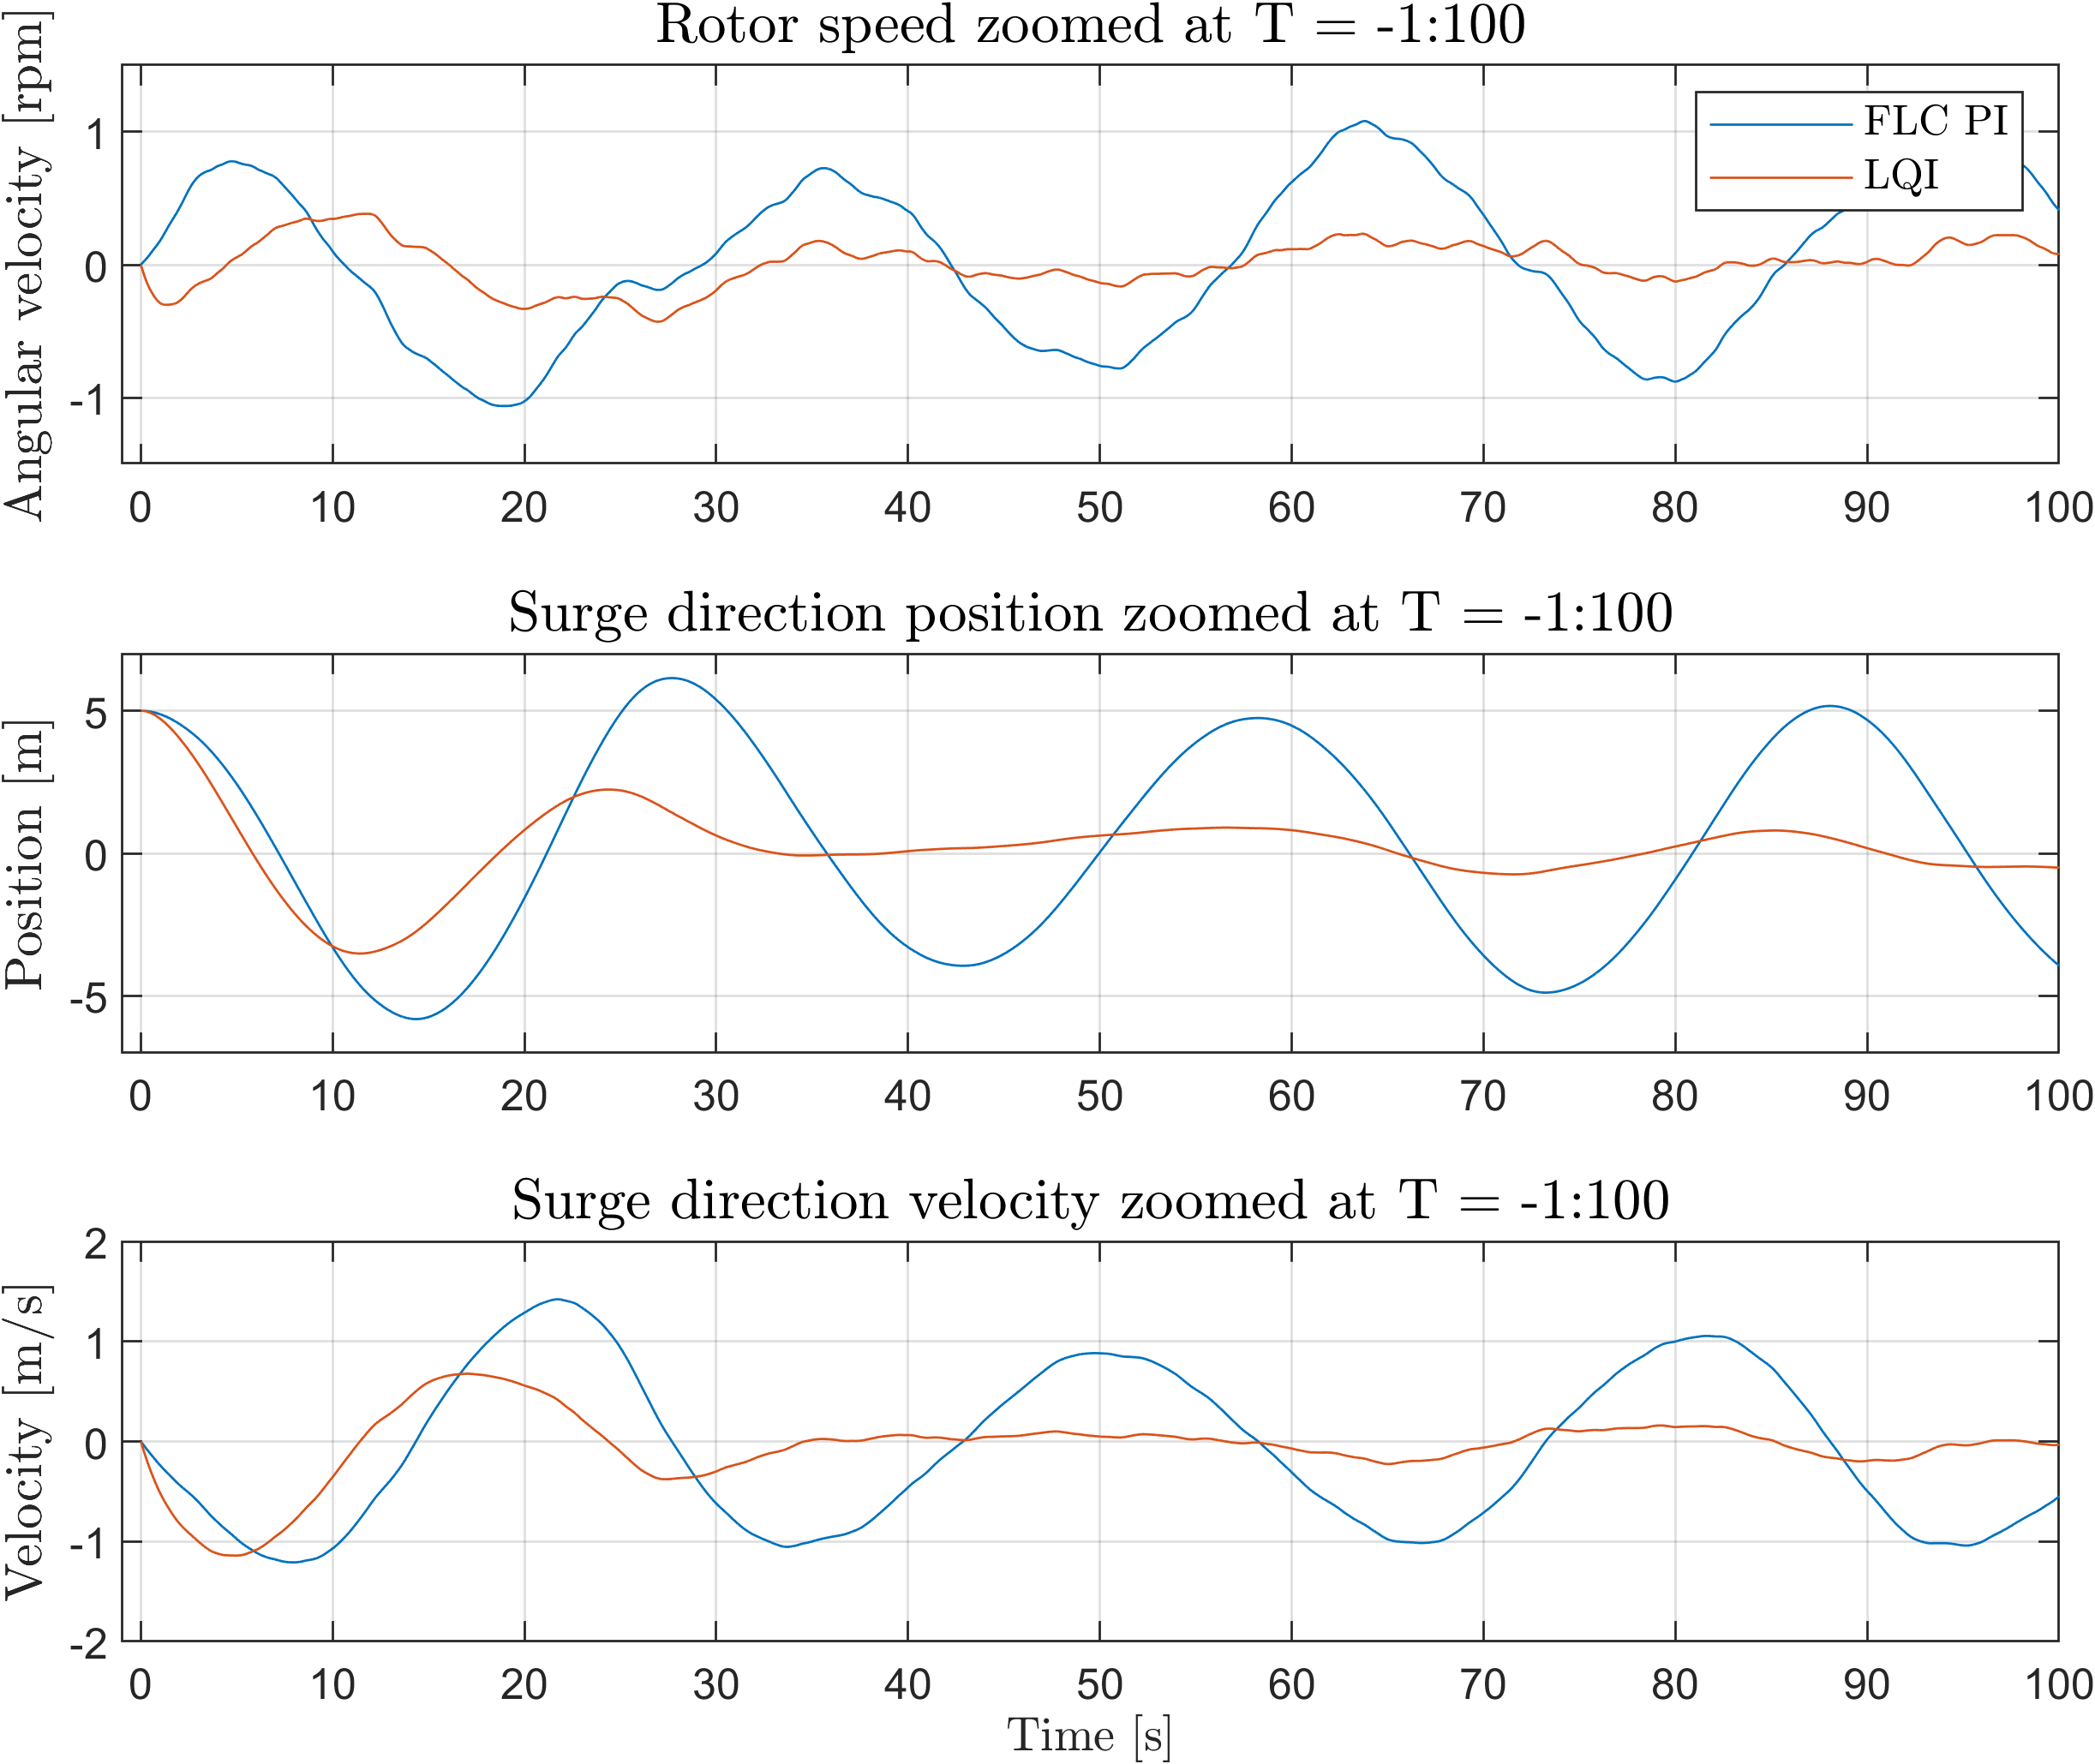
\includegraphics[width=0.7\linewidth]{Graphics/TestResults/linearModPerf/sim_12_W_py_vy_comp_zoom.png}
	\caption{Simulink simulation results zoomed in at the first 100 seconds where the fore-aft position is initialized at 5 m.}
	\label{fig:app_sim_12_W_py_vy_comp_zoom}
\end{figure}

The LQI controller pitch reference deviation from the OP and its rate of change is plotted in \cref{fig:app_sim_10_pitch}. Both the absolute value of the pitch reference and its rate of change should not exceed values which are realistic for the wind turbine at the OP. Simulations of the turbine in VTS has shown that a blade pitch rate of change of 2 deg/s and an absolute pitch deviation from the OP of 3-4 is fairly common. In the initial transient where the fore-aft position deviates by 5 m the pitch reference starts at 6 degrees and decreases with a rate og change starting at close to -3 deg/s. Neither the rate of change nor the absolute value are deemed problematic especially because such an abrupt change would not occur in a realistic scenario. For the remainder of the simulation the absolute value of the pitch reference deviation stays below 4 deg and the rate of change absolute value stays below 2 deg/s. These values are well inside an acceptable range.
\begin{figure}[ht]
	\centering
	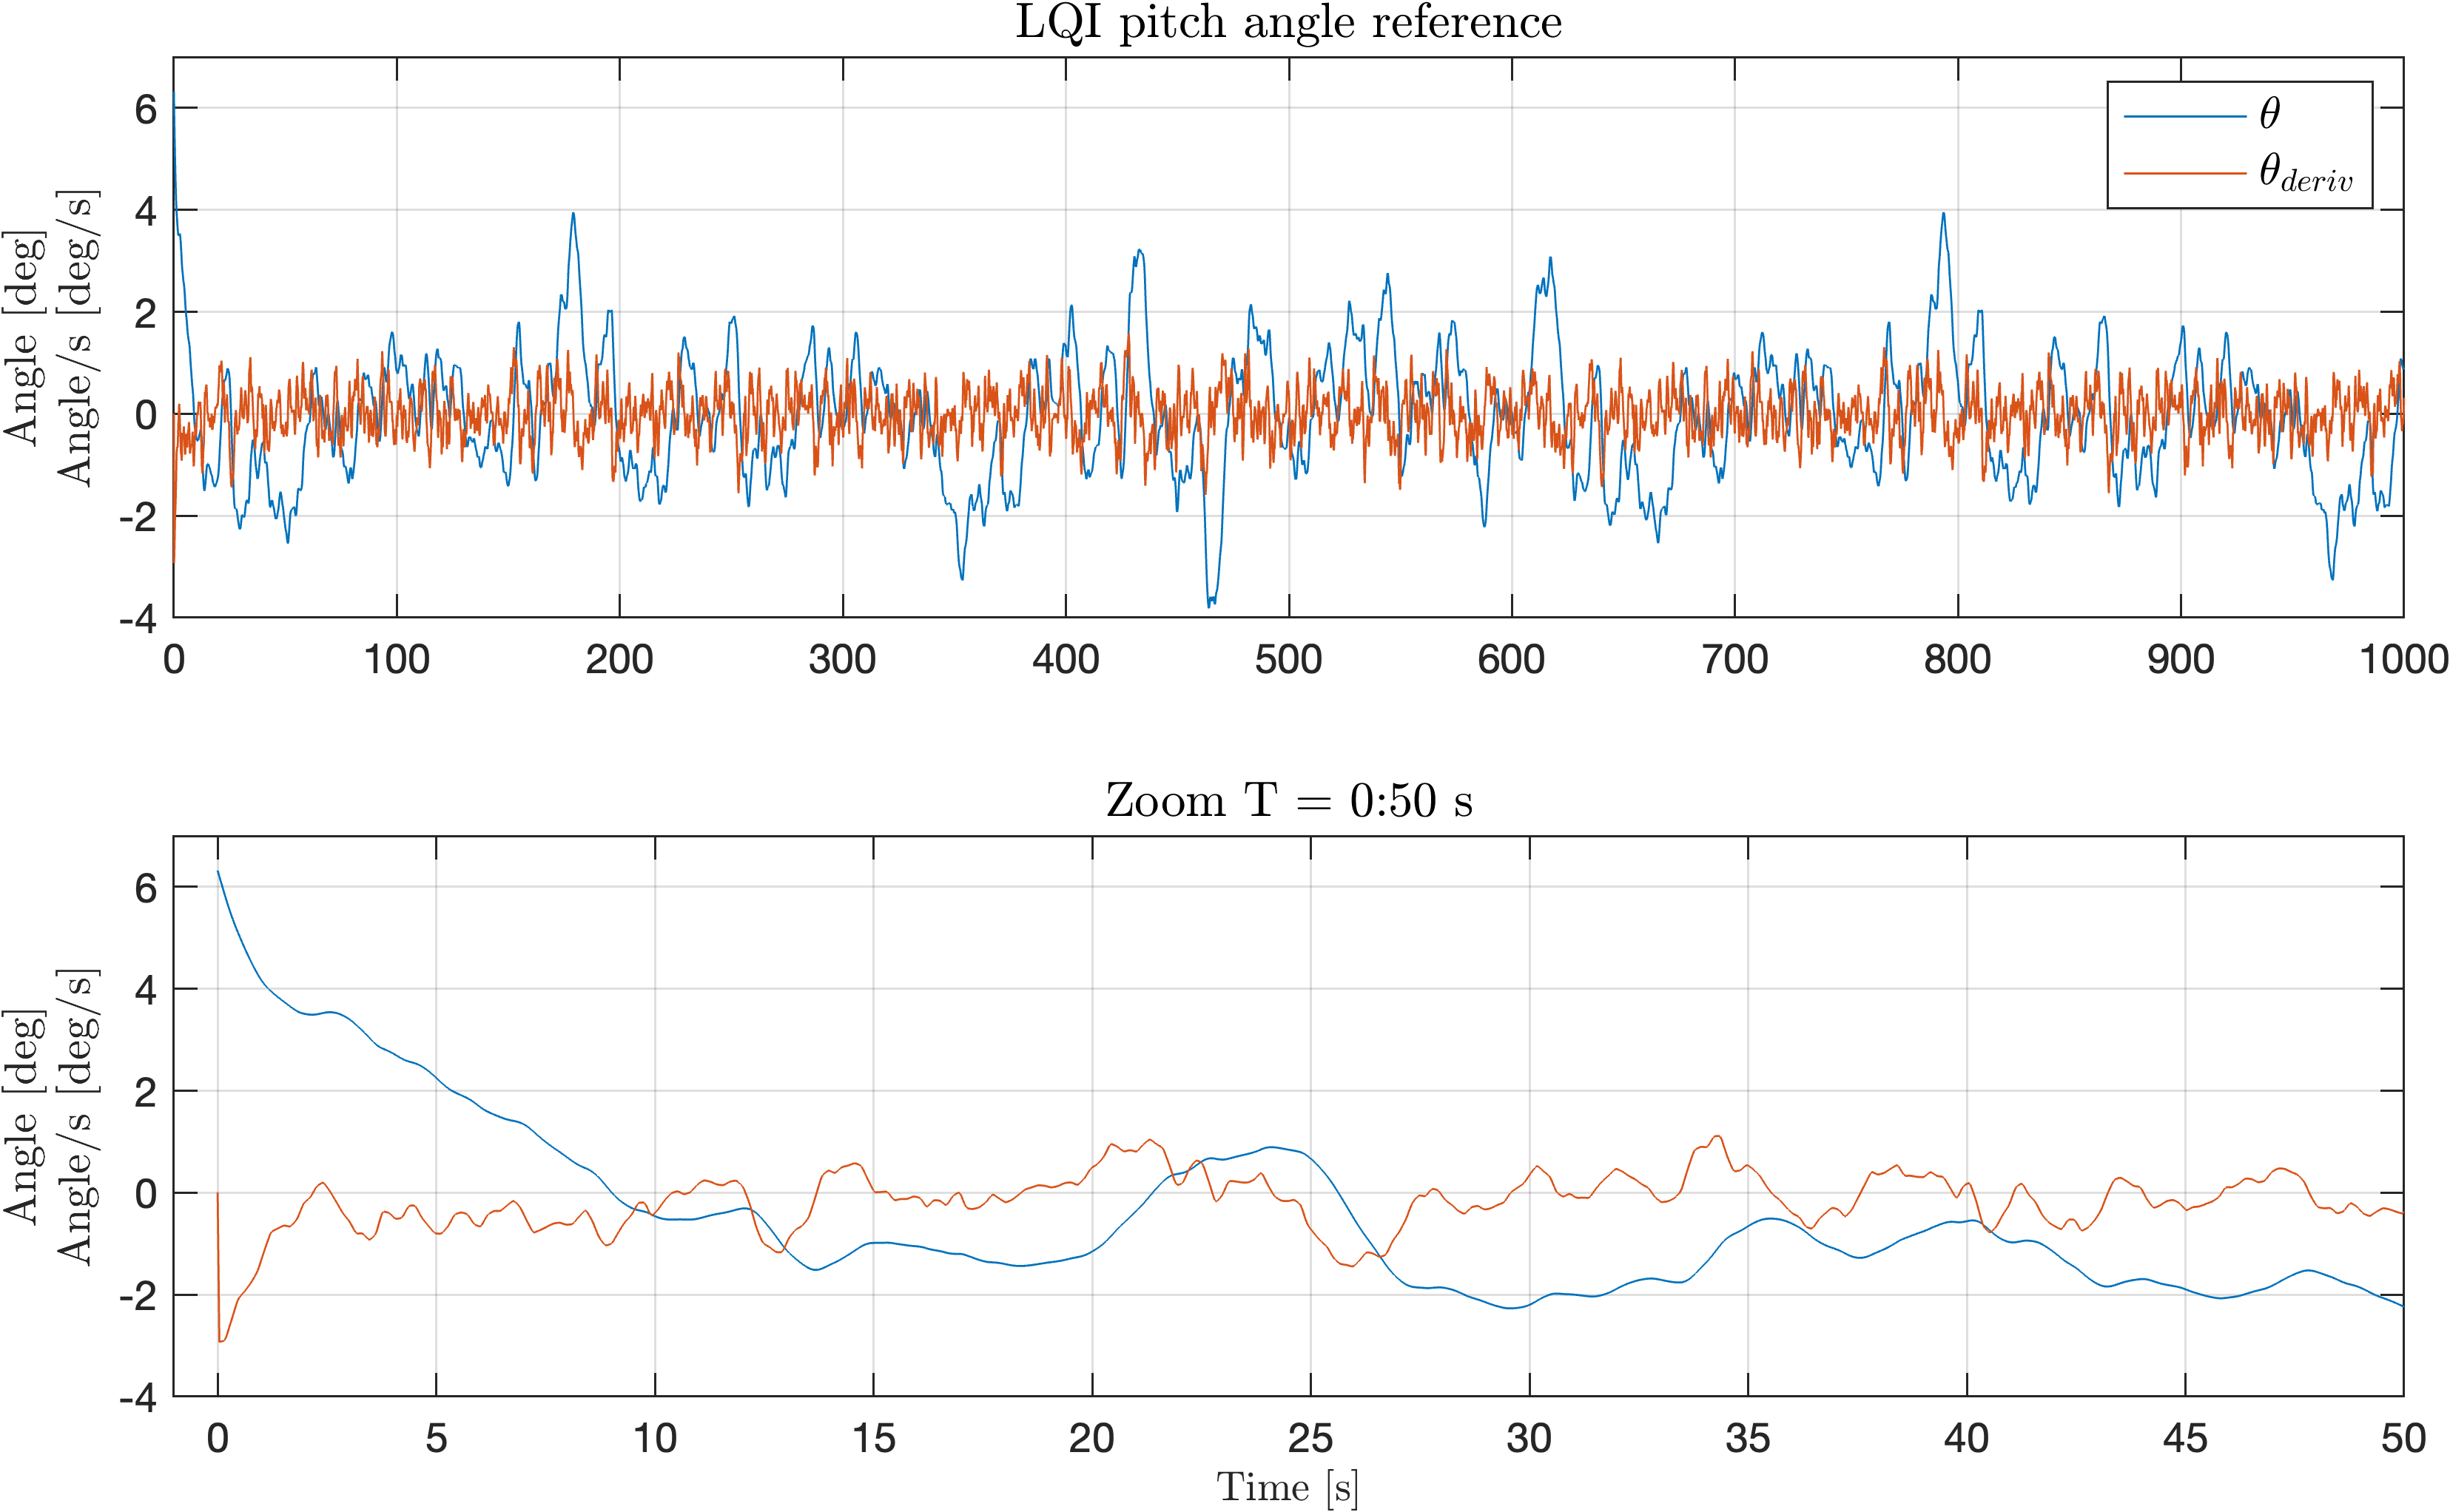
\includegraphics[width=0.7\linewidth]{Graphics/TestResults/linearModPerf/sim_10_pitch.png}
	\caption{Simulink simulation results of the pitch reference and pitch reference change. Neither the absolute value of the pitch reference nor the change in pitch reference reach alarming values.}
	\label{fig:app_sim_10_pitch}
\end{figure}

Conclusively the LQI controller performance is very good on the linear model in comparison to the FLC PI controller.% This is also to be expected given the...


% OLD PLOTS WITH vfree STEP
%\begin{figure}[ht]
%	\centering
%	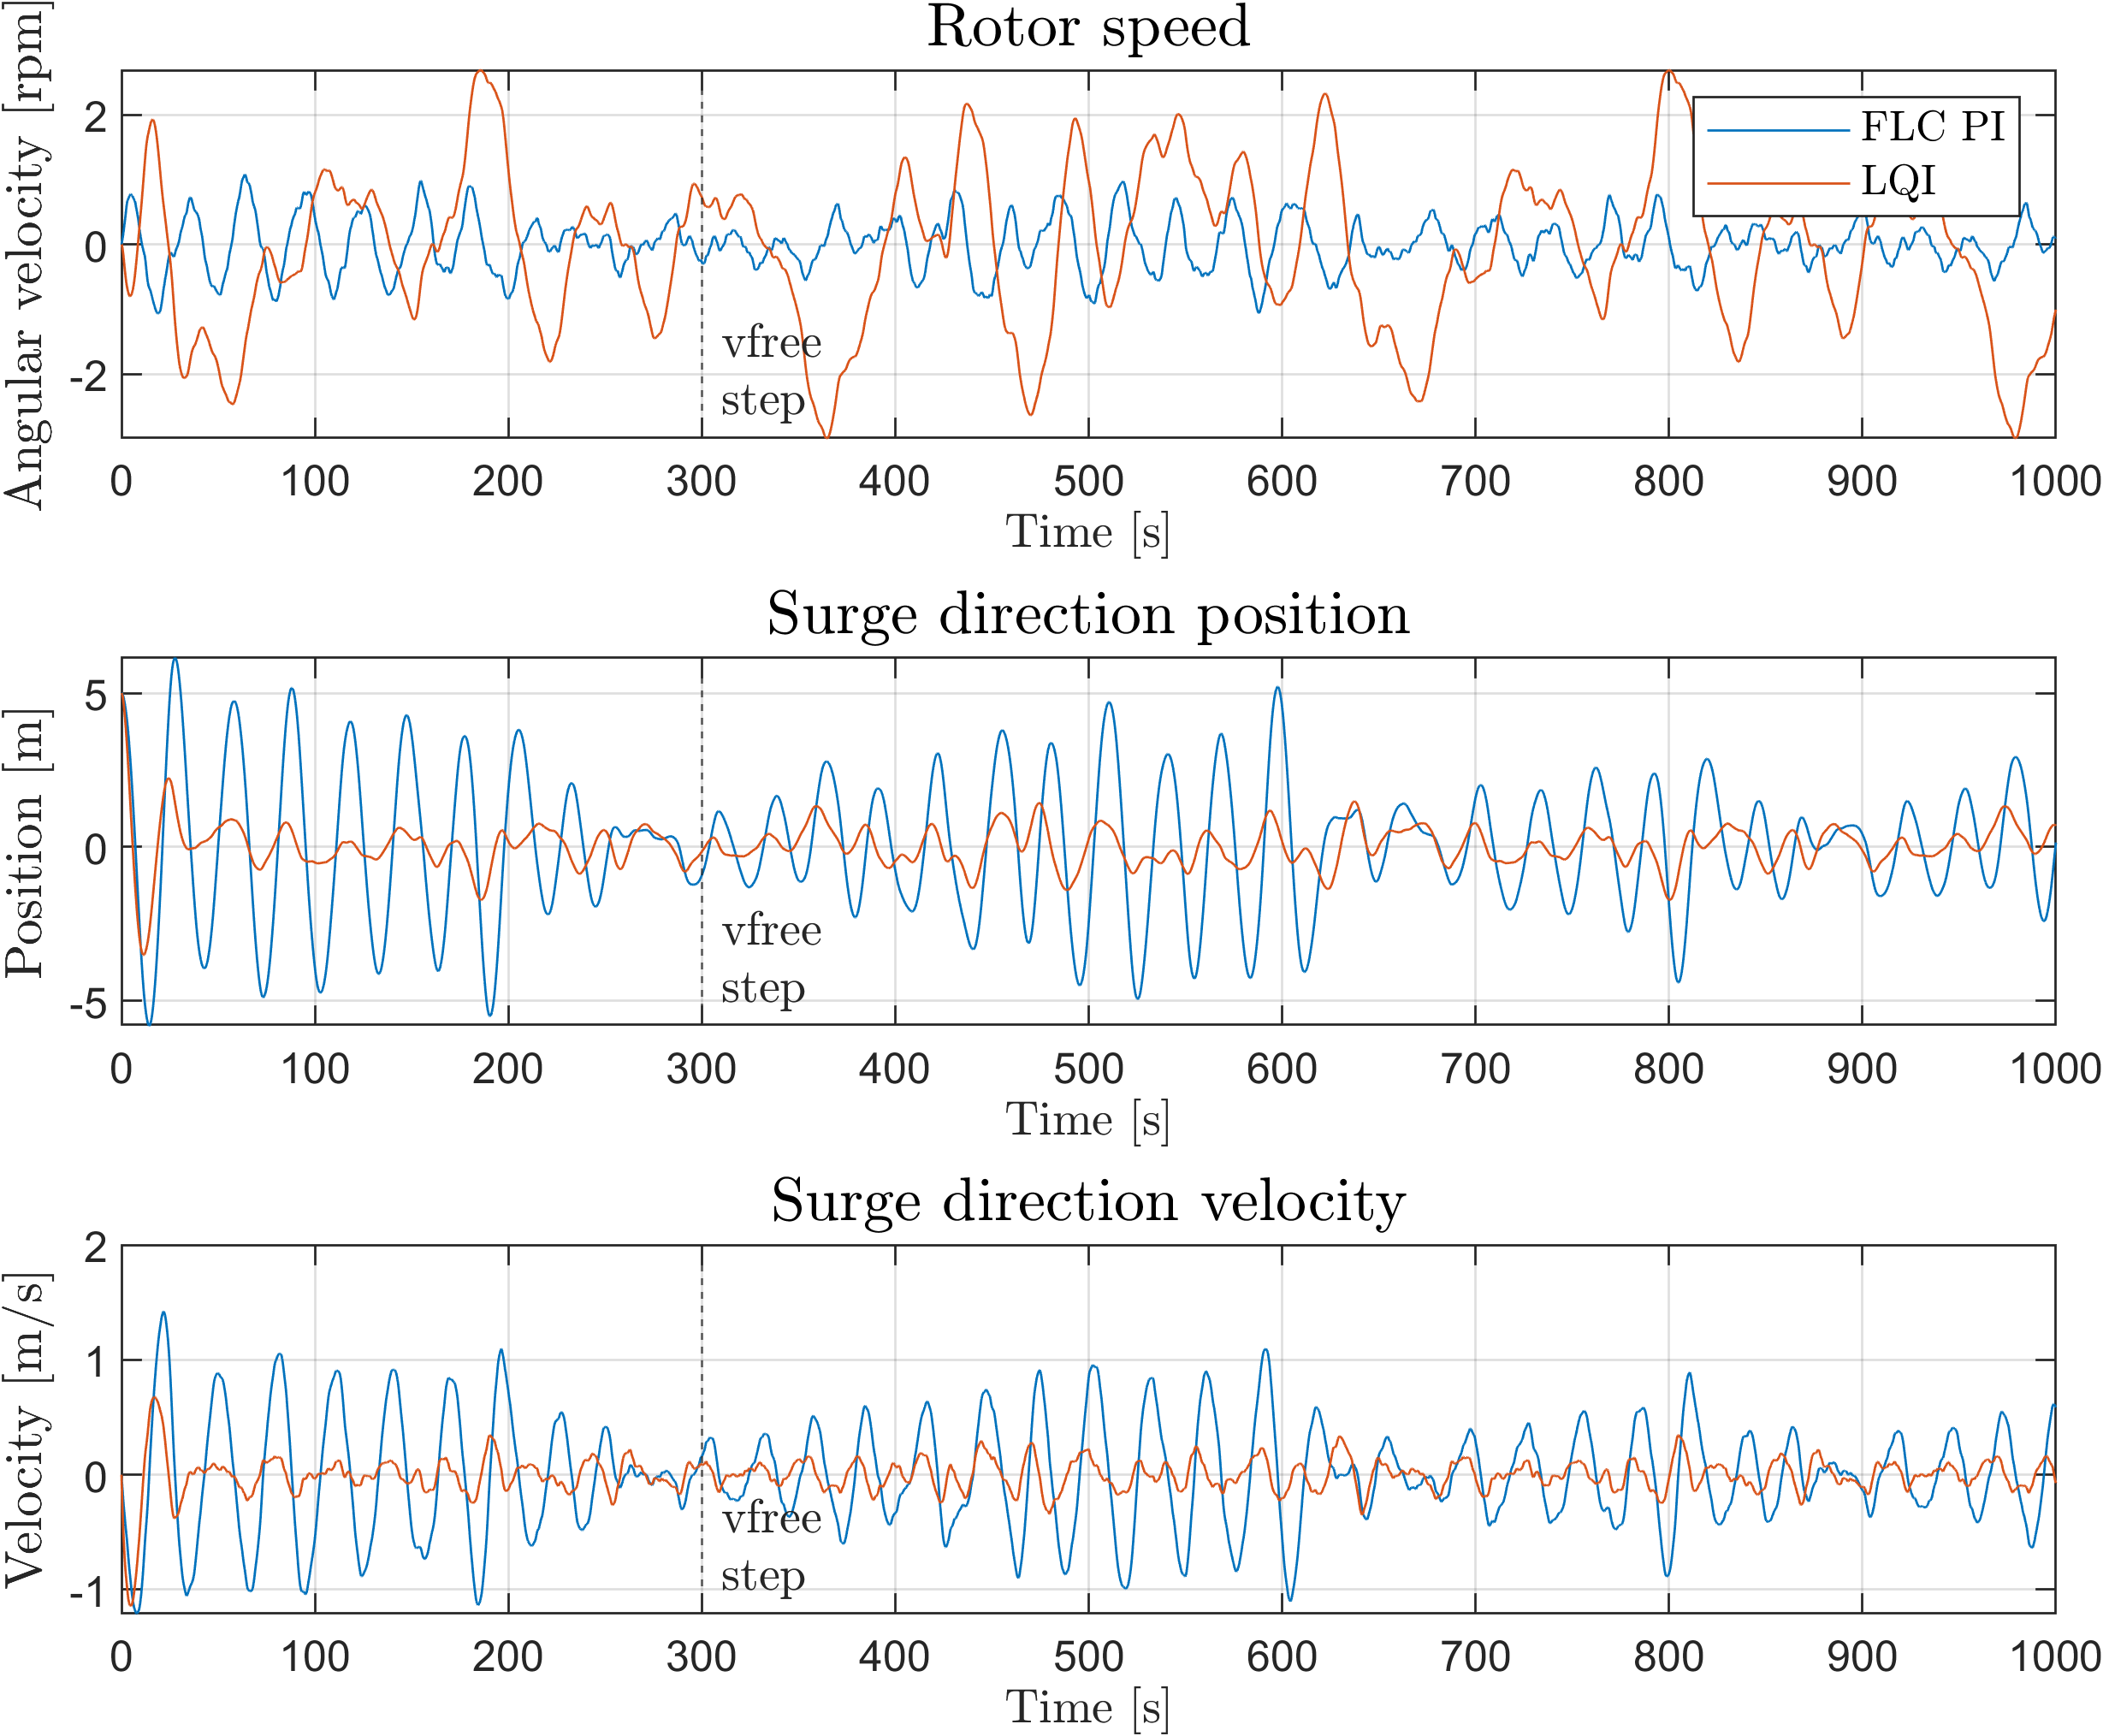
\includegraphics[width=0.7\linewidth]{Graphics/TestResults/linearModPerf/sim_02_W_py_vy_comp.png}
%	\caption{Simulink simulation results. The 10 m deviation initialization of the tower top position is visible from the \textit{fore-aft position} at 0 s.}
%	\label{fig:app_sim_02_W_py_vy_comp}
%\end{figure}
%
%\begin{figure}[ht]
%	\centering
%	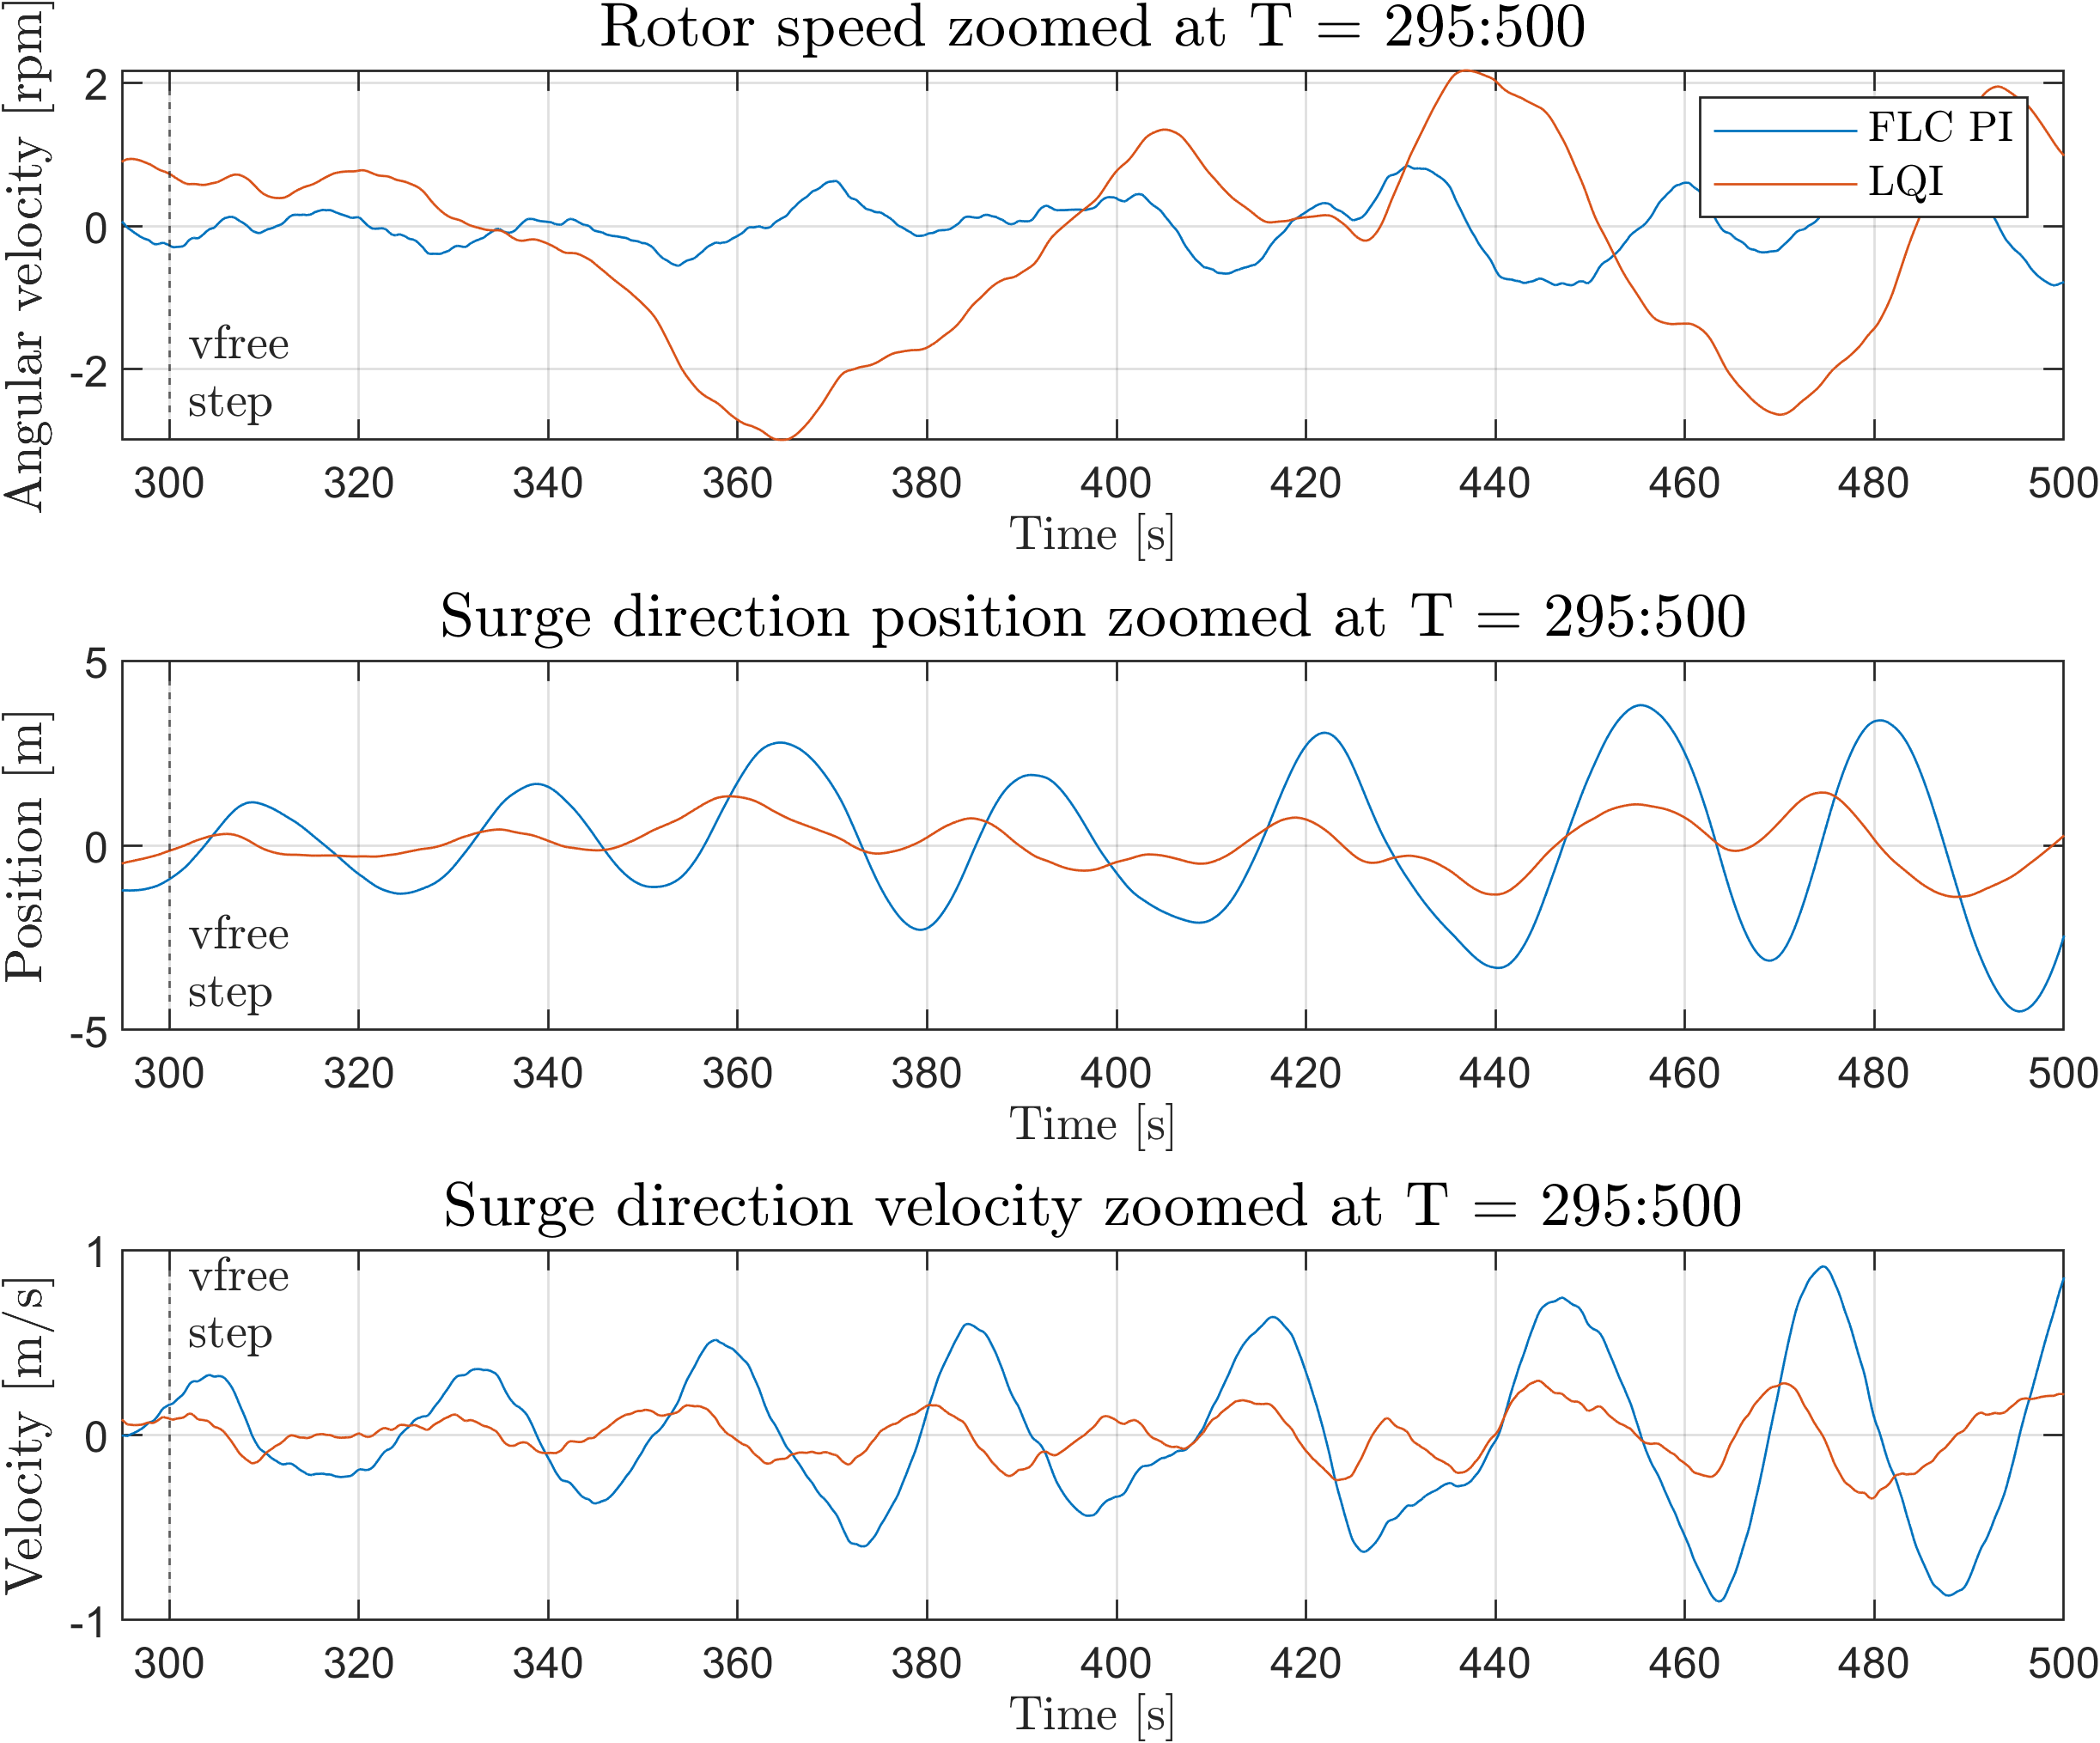
\includegraphics[width=0.7\linewidth]{Graphics/TestResults/linearModPerf/sim_03_W_py_vy_comp_zoom.png}
%	\caption{Simulink simulation results. Zoom at the disturbance step.}
%	\label{fig:app_sim_03_W_py_vy_comp_zoom}
%\end{figure}
%
%\begin{figure}[ht]
%	\centering
%	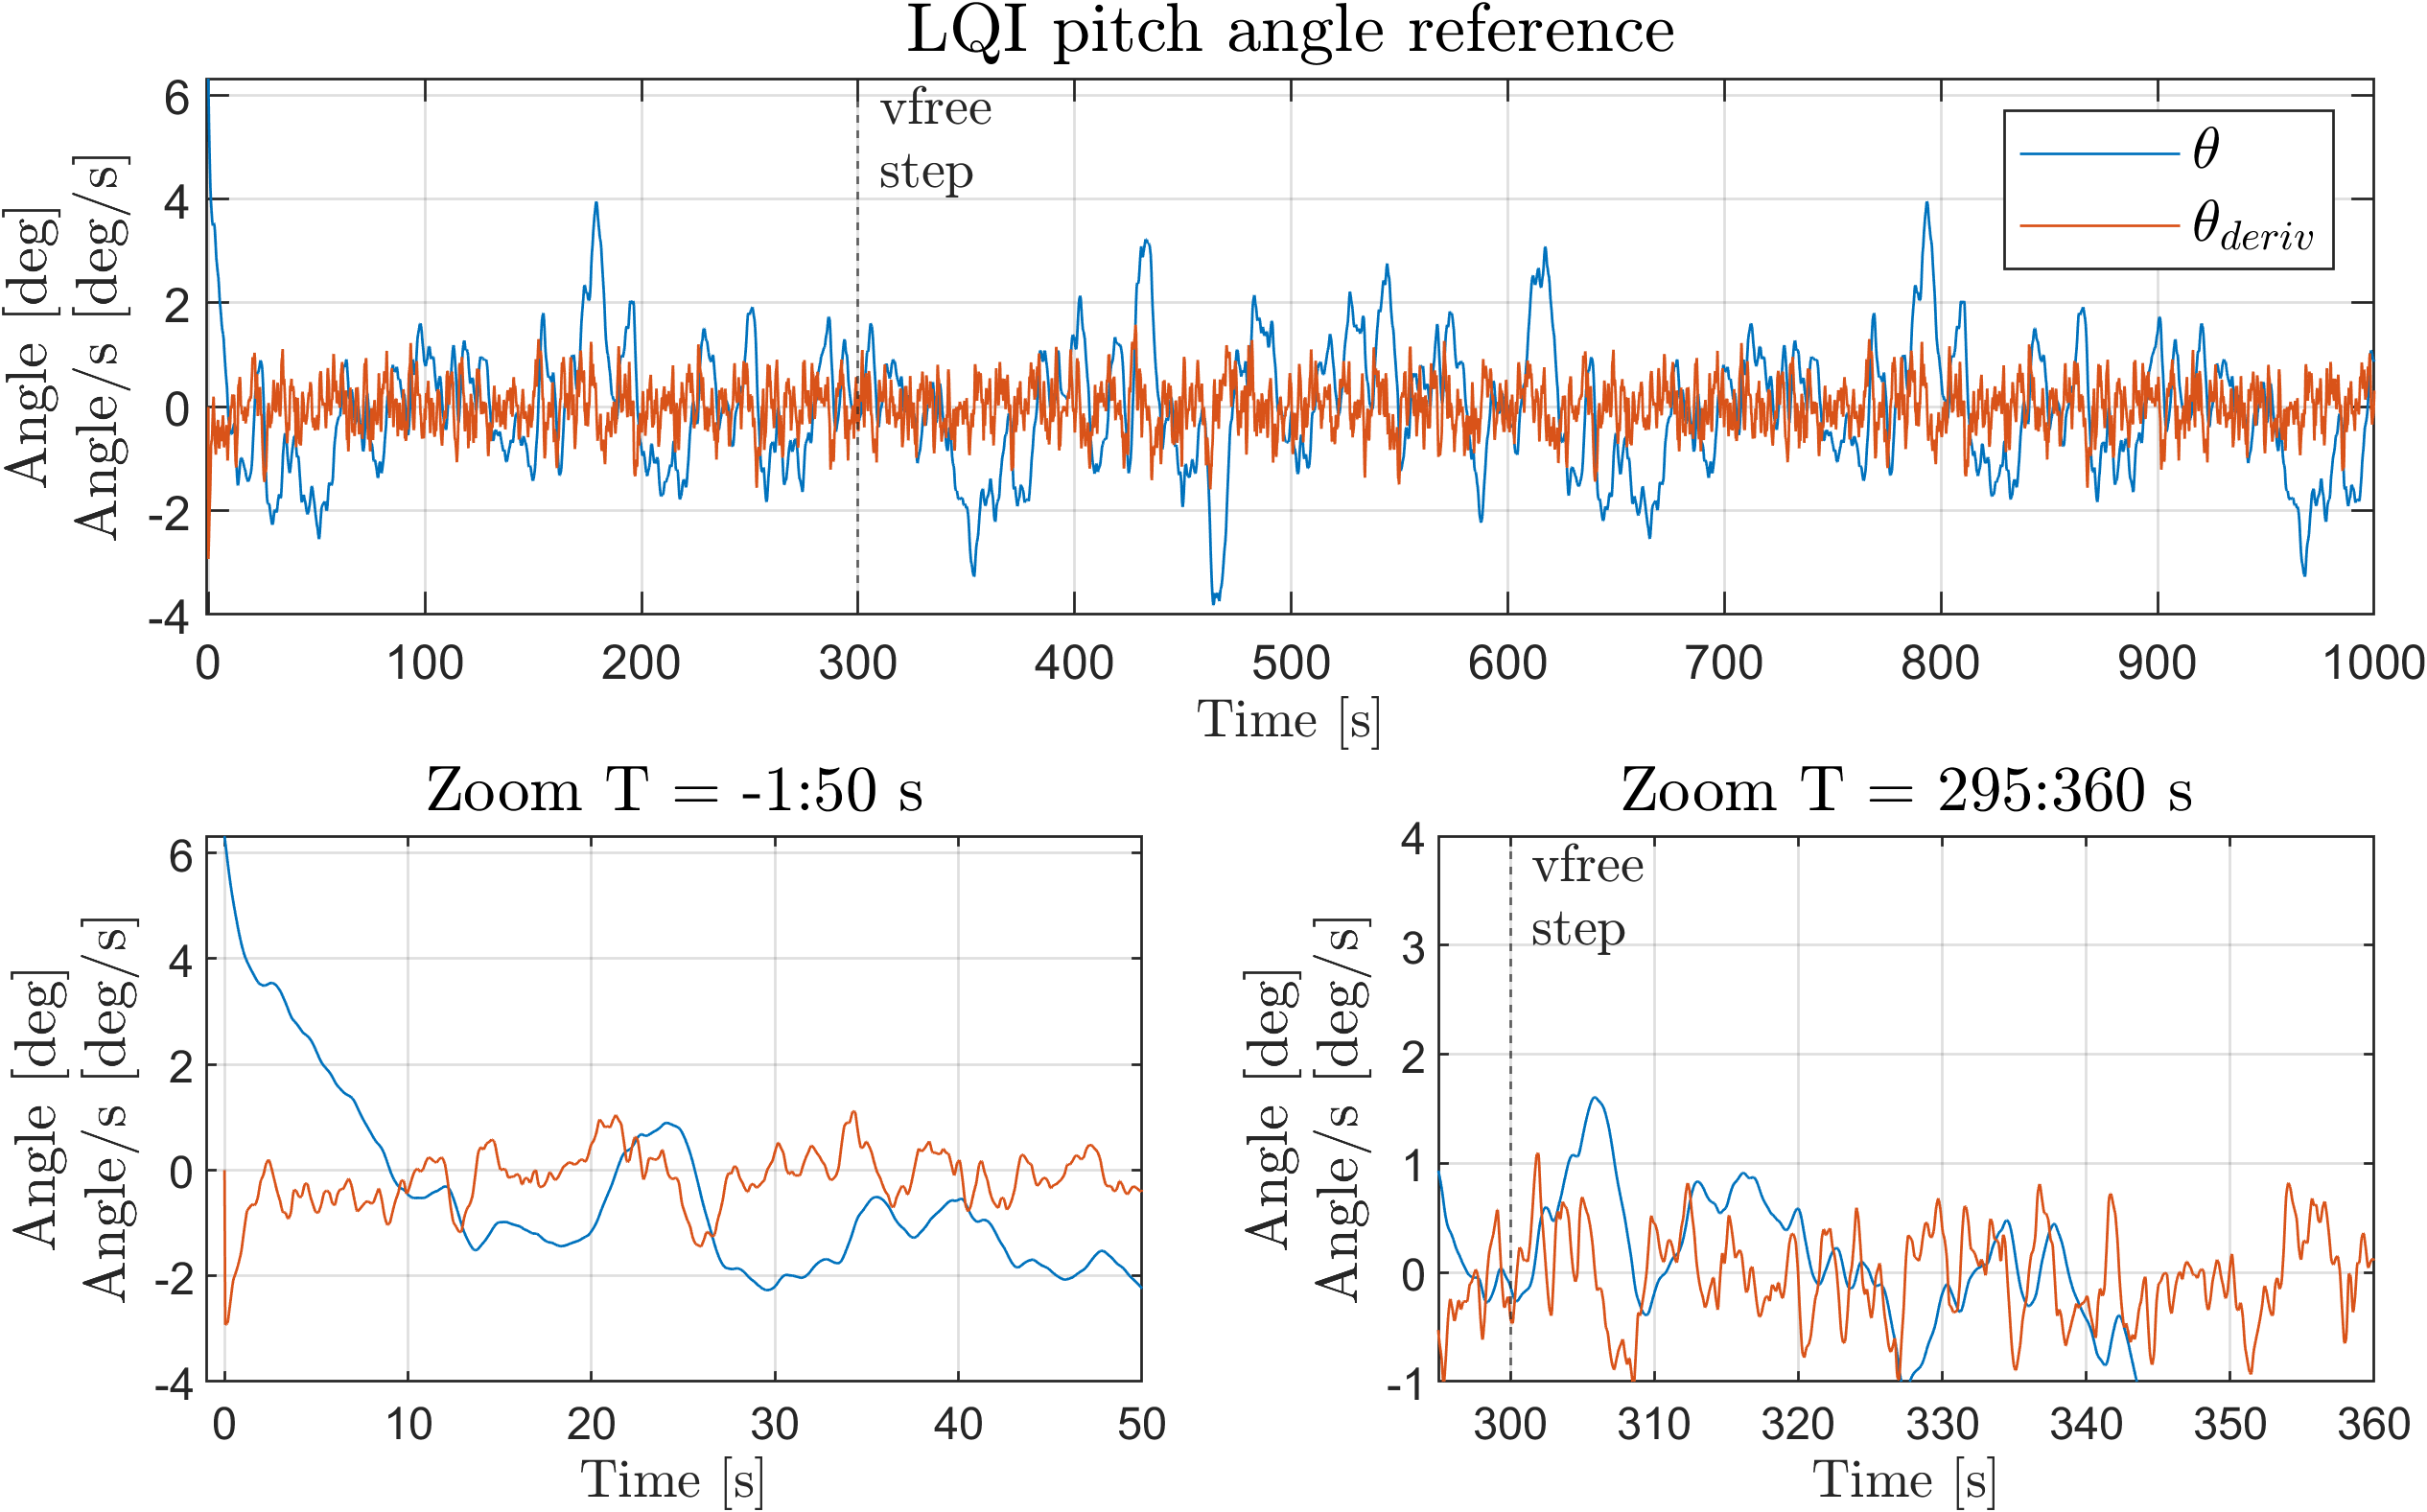
\includegraphics[width=0.7\linewidth]{Graphics/TestResults/linearModPerf/sim_01_pitch.png}
%	\caption{Simulink simulation results. Bottom left and right plots are zommed in at 0 to 50 s and 295 to 360 s.}
%	\label{fig:app_sim_01_pitch}
%\end{figure}


\subsection{Excluded component models} \label{sec:app_excl_comp_models}
This appendix contains component models which contain dynamics that from an understanding-the-theory POV are interesting but otherwise deemed unnecessary for the control objective. This is simply due to the frequency separation between the generally higher frequencies of these dynamics and the very slow eigenfrequency of a floating structure.

\subsubsection{Drivetrain (flexible)} \label{sec:mod_drt_flex}
As mentioned in \cref{sec:intro_wtcomponents} the drivetrain connects the rotor with the generator through a gearbox. The flexible drivetrain is modelled with a dampener and a spring between the rotor and the gearbox. The model is then reduced by translating the dampener and spring from the generator side to the rotor side of the gearbox. As such the model ends up consisting of two inertias coupled through a spring with stiffness $ K $ and a dampener with dampening $ B $. Due to the introduced spring and damper it is necessary to model both the rotor and and generator angle.
\begin{align} 
	J_{g} \ddot{\theta}_{gL} & = B (\dot{\theta}_r - \dot{\theta}_{gL}) + K(\theta_r - \theta_{gL}) - T_{g} \label{eq:comp_comp_drivetrain_flex_1} \\
	J_{r} \ddot{\theta}_r & = B (\dot{\theta}_{gL} - \dot{\theta}_r ) - K(\theta_r - \theta_{gL}) + T_{r} \label{eq:comp_comp_drivetrain_flex_2}
\end{align}
Recall the relationship between derivatives:
\begin{align}
	\dot{\Omega} & = \ddot{\theta}_r \\
	\dot{\omega}_{L} & = \ddot{\theta}_{gL} \\
	\dot{\theta}_g & = \omega \\
	\dot{\theta}_r & = \Omega
\end{align}
%and
%\begin{align}
%	\dot{\theta}_g & = \omega \\
%	\dot{\theta}_r & = \Omega
%\end{align}
and
\begin{align}
	\dot{\theta}_g 	&= \left(\dfrac{N_g}{N_r}\right) \dot{\theta}_{gL} \label{eq:comp_comp_drivetrain_flex_mod_3} \\
	J_{gL} 			&= J_{g} \left(\dfrac{N_r}{N_g}\right)^2 \label{eq:comp_comp_inertiamap_flex}
\end{align}
Which leaves the flexible drivetrain model as:
%\begin{align} 
%	\dot{\omega}_{gL} & = \dfrac{-B \dot{\theta}_{gL} + K(\theta_r - \theta_{gL}) - T_{g}}{J_{g}} \label{eq:comp_comp_drivetrain_flex_mod_1} \\
%	\dot{\Omega} & = \dfrac{-B \dot{\theta}_{gL} -B - K(\theta_r - \theta_{gL}) + T_{r}}{J_{r}} \label{eq:comp_comp_drivetrain_flex_mod_2} \\
%\end{align}
\begin{align} 
	\dot{\omega} & = \dfrac{B \left(\Omega - \dfrac{N_r}{N_g}\omega\right) + K\left(\theta_r - \dfrac{N_r}{N_g} \theta_{g}\right) - T_{g}}{\left(\dfrac{N_r}{N_g}\right)^2 J_{g} \dfrac{N_r}{N_g} } \label{eq:comp_comp_drivetrain_flex_mod_1} \\
	\dot{\Omega} & = \dfrac{B \left(\dfrac{N_r}{N_g}\omega - \Omega \right) \omega + K\left(\dfrac{N_r}{N_g} \theta_{g} - \theta_r\right) + T_{r}}{J_{r}} \label{eq:comp_comp_drivetrain_flex_mod_2} \\
	\dot{\theta}_g & = \omega \\
	\dot{\theta}_r & = \Omega
\end{align}
The model is observed to be linear and thus no linearisation is necessary.

The component inputs are $ \{T_g, T_r\} $ and the outputs are $ \{\omega, \Omega\} $. 

\subsubsection{Pitch system dynamics} \label{sec:comp_pitch_dyn}
The pitch system dynamics can be approximated with a simple first order low-pass filter which in the frequency domain is:
\begin{equation}\label{eq:comp_pitch_freq_dyn}
	\theta(s) = \dfrac{1}{\tau_{pit} s + 1} (\theta_{ref}(s) + \theta_{fatd}(s))
\end{equation}
where $ \tau_{pit} $ is a time-constant which suits the response of the pitching system at the operating point. In VTS the pitch system dynamics are modelled from a table which takes in the flap-wise bending moment of the blade and a pitch angle and outputs a pitch angle rate of change. As such wtLin uses the operating point and a user defined flap-wise bending moment to calculate $ \tau_{pit} $.

In the time domain the model becomes:
\begin{equation}\label{eq:comp_pitch_time}
	\dot{\theta} =\dfrac{(\theta_{ref}(s) + \theta_{fatd}(s)) - \theta}{\tau_{pit}}
\end{equation}

% The calculation of the time-domain version:
%\begin{align}\label{eq:comp_pitch}
%	\theta(s) & = \dfrac{1}{\tau_{pit} s + 1} (\theta_{ref}(s) + \theta_{fatd}(s)) \\
%	(\tau_{pit} s + 1) \theta(s) & = (\theta_{ref}(s) + \theta_{fatd}(s)) \\
%	\tau_{pit}\theta s + \theta(s)  & = (\theta_{ref}(s) + \theta_{fatd}(s)) \\
%	\tau_{pit}\dot{\theta} + \theta  & = (\theta_{ref}(s) + \theta_{fatd}(s)) \\
%	\dot{\theta} & =\dfrac{(\theta_{ref}(s) + \theta_{fatd}(s)) - \theta}{\tau_{pit}}
%\end{align}

The component inputs are $ \{\theta_{ref}, \theta_{fatd}  \} $ and the output is $ \{\theta \} $


\subsubsection{Generator} \label{sec:comp_generator_eff}
The generator is mechanically connected to the drivetrain and is electrically connected to the converter. It is used to control the rotor speed during PLC by means of the generator torque.

A more detailed generator model could include efficiencies. In Vestas' turbine simulator (VTS) the generator efficiencies are defined in tables and are dependent on grid output power $ P $ and generator speed $ \omega $. The output is three respective output efficiencies: 
\begin{enumerate}
	\item Mechanic efficiency: $ \eta_m(P,\omega) $
	\item Electric efficiency: $ \eta_e(P,\omega) $
	\item Auxiliary efficiency: $ \eta_a(P,\omega) $
\end{enumerate}
Where 
\begin{equation}\label{eq:comp_gen_effi_eff}
	\eta(P,\omega) = \eta_m(P,\omega) + \eta_e(P,\omega) + \eta_a(P,\omega)
\end{equation}
From the total efficiency the output grid power is:
\begin{equation}\label{eq:comp_gen_elec_pow_eff}
	P_{gen} \eta(P,\omega) = P
\end{equation}
where $ P_{gen} $ is the electrical power output of the generator.

This leaves the power loss from generator to grid to be defined as:
\begin{equation} \label{eq:comp_gen_pow_loss_eff}
	P_{loss}(P, \omega) = P_{gen} - P = \dfrac{P}{\eta(P, \omega)} - P
\end{equation}
The power of a rotating machine can be defined as the product of torque and rotational velocity:
\begin{equation}\label{eq:comp_power_in_rot_eff}
	P_{gen} = T_g \omega
\end{equation}
As such for the system at hand the torque can be defined by rearranging \cref{eq:comp_power_in_rot_eff} and substituting in $ P_{gen} $ from \cref{eq:comp_gen_pow_loss_eff}. This leaves the non-linear generator model to be:
\begin{equation}\label{eq:comp_gen_torque_eff}
	T_g(P, \omega) = \dfrac{P_{loss}(P, \omega) + P}{\omega}
\end{equation}
\cref{eq:comp_power_in_rot_eff} is the non-linear model of the generator. It contains $ P_{loss}(P,\omega) $ which from \cref{eq:comp_gen_pow_loss_eff} is dependent on $ \eta(P, \omega) $. The $ \eta $ function is extracted from VTS and linearized.

The linear model of the generator is obtained through a taylor expansion. The notation is relaxed a bit such that $ P_{loss}( P, \omega) $ is simply expressed as $ P_{loss} $.
\begin{equation}\label{eq:comp_taylor_eff}
	T_g( P, \omega) \approx T_g(P_o, \omega_o) + 
	\left. \dfrac{\partial T_g( P, \omega)}{\partial P} \right |_{P_o,\omega_o} ( P-P_o) + 
	\left. \dfrac{\partial T_g( P, \omega)}{\partial \omega} \right |_{P_o,\omega_o} (\omega - \omega_o)
\end{equation}
Below the the generator torque sensitivity to the grid power change term from \cref{eq:comp_taylor_eff} is derived. From \cref{eq:comp_gen_1_1_eff} to \cref{eq:comp_gen_1_2_eff} the \textit{sum rule} is used to split the derivative into two added derivatives. From \cref{eq:comp_gen_1_2_eff} to \cref{eq:comp_gen_1_3_eff} the first fractions in the denominators of the partial derivatives of the two terms are treated as a product of two functions thus the \textit{product rule} is used. The assumption is that the grid power is completely disconnected from the generator through the converter. Thus from \cref{eq:comp_gen_1_3_eff} to \cref{eq:comp_gen_1_4_eff} $ \, \frac{\partial \, \omega^{-1}}{\partial P} = 0 $.
\begin{align} 
	\dfrac{\partial T_g( P, \omega)}{\partial P} &= \dfrac{\partial \left (\dfrac{P_{loss} +  P}{\omega}\right )}{\partial P} \label{eq:comp_gen_1_1_eff} \\
	& = \dfrac{\partial \left (\dfrac{P_{loss}}{\omega} \right )}{\partial P} + \dfrac{\partial \left ( \dfrac{ P}{\omega} \right )}{\partial P} \label{eq:comp_gen_1_2_eff} \\
	& = \dfrac{1}{\omega} \cdot \dfrac{\partial P_{loss}}{\partial P} + \dfrac{\partial \left ( \dfrac{1}{\omega} \right )}{\partial P} P_{loss} + \dfrac{1}{\omega} \cdot \dfrac{\partial P}{\partial P} + \dfrac{\partial \left (\dfrac{1}{\omega} \right )}{\partial P}  P \label{eq:comp_gen_1_3_eff} \\
	& = \dfrac{1}{\omega} \cdot \dfrac{\partial P_{loss}}{\partial P} + \dfrac{1}{\omega} \label{eq:comp_gen_1_4_eff}
\end{align}


The generator torque sensitivity to rotational velocity change from \cref{eq:comp_taylor_eff} is then derived:
\begin{align}
	\dfrac{\partial T_g(P, \omega)}{\partial \omega} & = \dfrac{\partial \left (\dfrac{P_{loss} +  P}{\omega}\right )}{\partial \omega} \\
	& = \dfrac{\partial \left (\dfrac{P_{loss}}{\omega} \right )}{\partial \omega} + \dfrac{\partial \left (\dfrac{P}{\omega} \right )}{\partial \omega} \\
	& = \dfrac{1}{\omega} \cdot \dfrac{\partial P_{loss}}{\partial \omega} + \dfrac{\partial \left (\dfrac{1}{\omega} \right)}{\partial \omega} P_{loss} + \dfrac{1}{\omega} \dfrac{\partial P}{\partial \omega} + \dfrac{\partial \left (\dfrac{1}{\omega} \right )}{\partial \omega} P \\
	& = \dfrac{1}{\omega} \cdot  \dfrac{\partial P_{loss}}{\partial \omega} - \dfrac{1}{\omega^2}(P + P_{loss}) + \dfrac{1}{\omega} \dfrac{\partial P}{\partial \omega} \\
	& = -\dfrac{1}{\omega^2}(P + P_{loss}) + \dfrac{1}{\omega} \cdot \dfrac{\partial P_{loss}}{\partial \omega}
\end{align}
The above derived generator model is referred to the low-speed generator side by replacing $ \omega $ with $ \omega_L $ where $ \omega_L = \left (\frac{N_r}{N_g} \right ) \omega $. This yields the final linear generator model evaluated at the operating point $ (P_o, \omega_o) $. Furthermore $P_{loss}$ is still just a function of $ \omega_L $ and $ P $:
\begin{equation}
	\begin{split}
		T_g(P, \omega_L) 	& \approx \left. \left ( \dfrac{1}{\omega_L} \cdot \dfrac{\partial P_{loss}(P, \omega_L)}{\partial P} + \dfrac{1}{\omega_L} \right ) \right |_{P_o,\omega_{L_o}} (P - P_0) \\ 
		& + \left ( -\dfrac{1}{\omega_L^2}(P + P_{loss}(P, \omega_L)) + \left. \dfrac{1}{\omega_L} \cdot \dfrac{\partial P_{loss}(P, \omega_L)}{\partial \omega_L} \right ) \right |_{P_o,\omega_{L_o}} (\omega_L - \omega_{L_o})
	\end{split}
\end{equation}
The calculation of the power loss and derivation of the power loss sensitivity to grid power are left out here, but are calculated in wtLin at an operating point. In the wtLin tool these sensitivities are calculated based on the extracted tables of efficiency $ \eta $.

Presently the generator model in wtLin is implemented assuming a stiff drivetrain such that $ \Omega = \omega_L $.

The component model input is $ \{P, \Omega\} $ and the output is $ \{T_g\} $


\clearpage
\section{Documentation and tests}
\subsection{Test Journal: Preliminary VTS model frequency sweep} \label{app:tj_00}

\textbf{Executed by: Martin Therkildsen} \\
\textbf{Date: 05/10/2022}

\subsubsection{Objective}
This test aims to document the behaviour of the floating Vestas Turbine Simulator (VTS) model in the first semi-successful preliminary frequency sweep test. It is desired to get an understanding of how the floating turbine is operating when the different rotor frequencies are induced and how these frequencies translate into the structure of the turbine.

\subsubsection{Background}
A Vestas matlab tool called SysIdFrqSweep is able to generate Design Load Cases (DLCs) which make a variable such as the rotor speed include a constant frequency as to analyse how such a frequency translates to the rest of the system mainly of interest the y-direction foundation translation and tower pitch angle. Essentially it should be possible to make a bode plot when enough simulations are run at enough frequencies. This could be used to tune the linear model to match the VTS model as closely as possible. As such bode plots would also be made for the linear model and compared.

\subsubsection{Test subject}
The test subject is a specific floating turbine setup which is simulated with VTS. The turbine is a V164 8MW on a floating semi-submersible platform.

\subsubsection{Equipment/Software used and test setup}
The software used for this test is:
\begin{itemize}
	\item \textbf{fat1}: Vestas' simulation prepping software
	\item \textbf{VTS}: Vestas' turbine simulator software
	\item \textbf{OrcaFlex}: A floating foundation simulation tool which communicates with VTS to make floating simulations
	\item \textbf{Matlab}: To make fast fourier transforms fft of the data and to plot the data in figures
	\item \textbf{SysIDFrqSweep matlab tool}: A Vestas matlab tool which generates load cases which are put into the turbine prep file to simulate variables oscillating at chosen frequencies
\end{itemize}


\subsubsection{Test procedure}
SysIdFrqSweep is used to generate in this test to generatoe 10 different frequencies which are to be applied to the rotor speed. These frequencies are merely put on top of the rotational velocity of the turbine rotor. The rotor will still act according to the simulated physical environment. As such when the tower pitches and moves around the rotor speed will still change accordingly.

The generated rotor frequencies which are generated  are: $0.01, 0.02 ... 0.1$.

The generated prep file is run through fat1 which prepares (preps) the file such that VTS and OrcaFlex can run the simulation. The simulation is set to run a 1800 second simulation.

When the simulation is finished several types of files are output which can be used to analyze what happened during the simulation. ".int" files are sensor file which are virtual sensor readings and products of treated sensors readings. Data from these files are the ones who are plotted in Matlab.

Errors occurred on frequencies 0.01 and 0.03 and as such these could not be plotted in this test. This leaves eight different frequencies.

In Matlab a script made by me extracts the data from the .int files by using a LaC matlab tool. A subset of data is made by fourier transforming all the data such that ffts can also be plotted. The data is then plotted in figures as results.


\subsubsection{Results and Comments}
Since there are 8 different frequencies the data is plotted in sets of four frequencies. Not all all plots of all frequencies are included. 

The first two plots are plots of the free wind speed, blade pitch angle 1, rotor angular velocity and generator torques for the two sets of four frequencies respectively. Frequencies 0.02 to 0.06 are seen in \cref{fig:tjj0_f02to06VfreeToMgen} and frequencies 0.07 to 0.1 are seen in \cref{fig:tjj0_f07to1VfreeToMgen}. The time is restricted to a 100 second window. It is seen that the wind speed is set unrealistically at a constant wind speed such that this disturbance would not interfere with the observations of the system frequencies. Only one blade pitch is plotted since it is deemed redundant to plot all pitch angles as they will all have the same angle at only slightly different amplitudes and slightly different phases. When observing the angular velocities it becomes evident that it is not a trivial task to read out the frequencies added on top of the rotor angular velocity in the timeseries. When observing the rotor angular velocity fft plots in \cref{fig:tjj0_f02to06OmegaFFT} and \cref{fig:tjj0_f07to1_OmegaFFT} the frequencies are apparent as pins at each of the respective frequencies. The frequency content observed at around 0.034 Hz is the natural frequency of the tower-foundation structure in the water.

It is widely evident that the turbine is pitching and translating in the water, resulting in great oscillations in the whole turbine. When looking at the plot of the tower translations and pitch angles in \cref{fig:tjj0_f07to1_xPosToPitchAng} it is obvious that the oscillations are occurring due to the structure movement. An fft of the roll and pitch angles are seen in \cref{fig:tjj0_f07to1_RollPitchAngFFT}.
\begin{figure}[h]
	\centering
	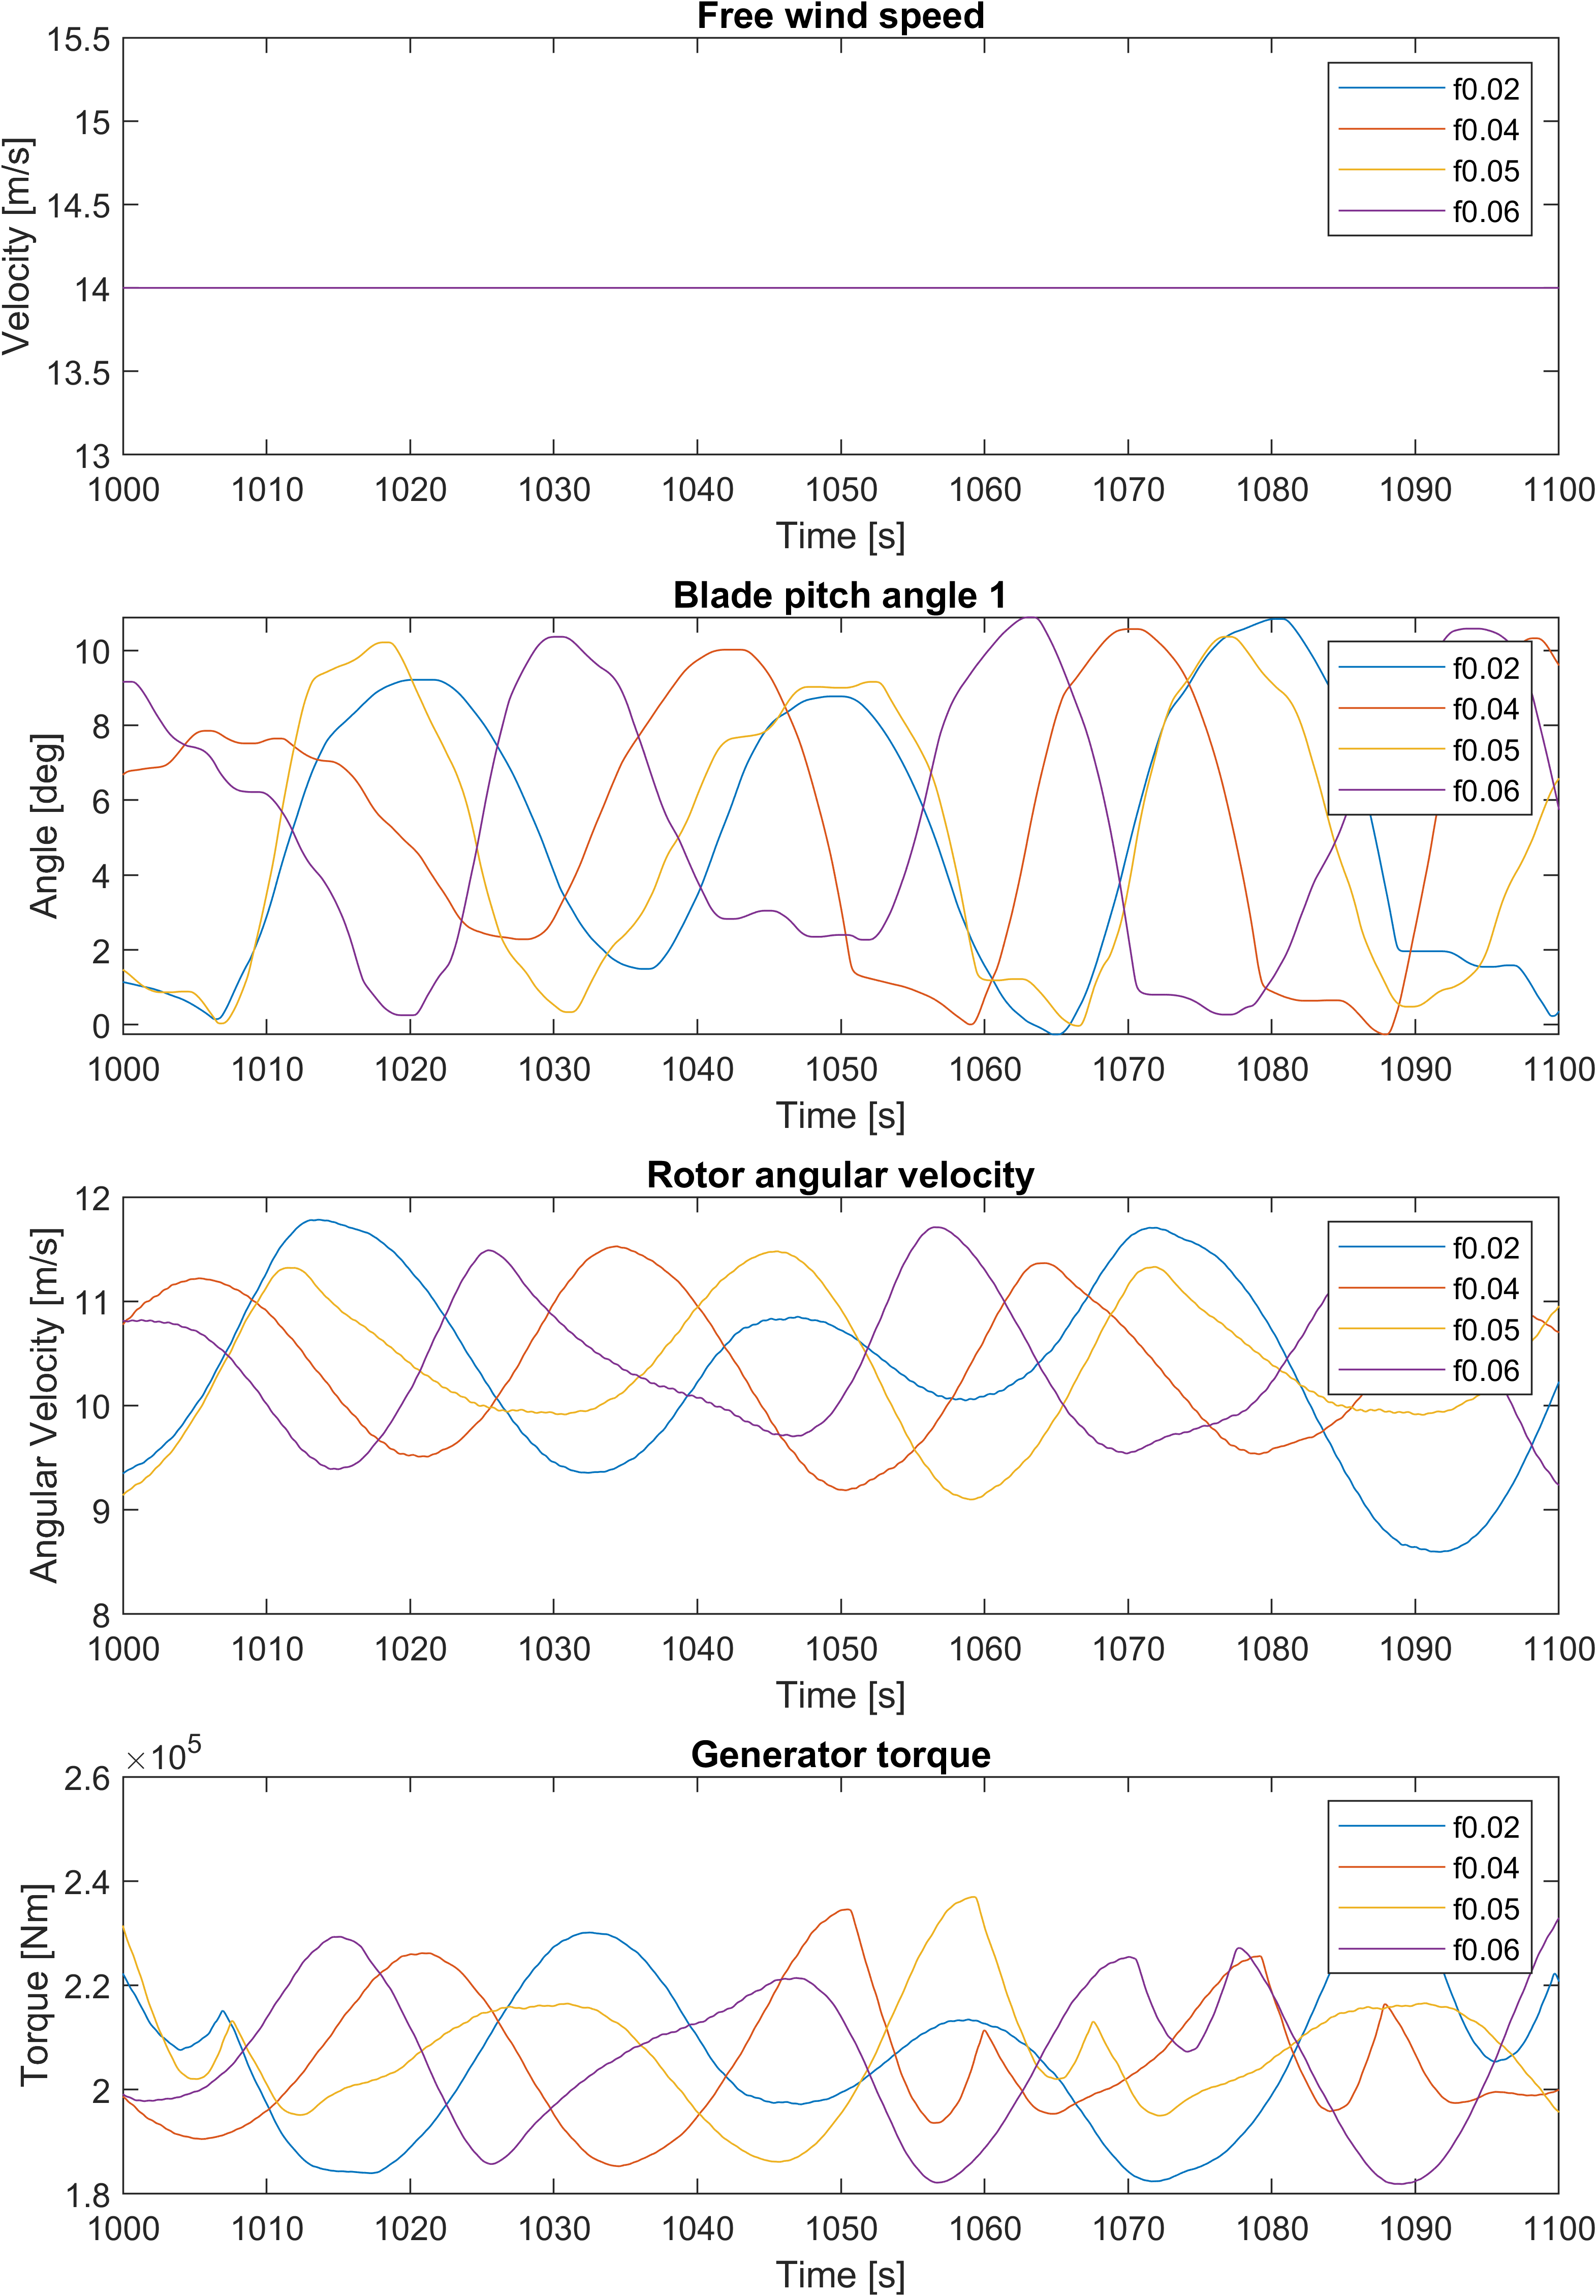
\includegraphics[width=0.8\linewidth]{Graphics/TestResults/tj00/tjj0_f02to06VfreeToMgen.png}
	\caption{Plot of Free wind, Blade pitch angle 1, rotor angular velocity and Generator torque for the injected rotor angular velocity frequencies 0.02 Hz, 0.04 Hz, 0.05 Hz and 0.06 Hz. It is difficult to observe the frequencies directly on the angular velocity.}
	\label{fig:tjj0_f02to06VfreeToMgen}
\end{figure}

\begin{figure}[h]
	\centering
	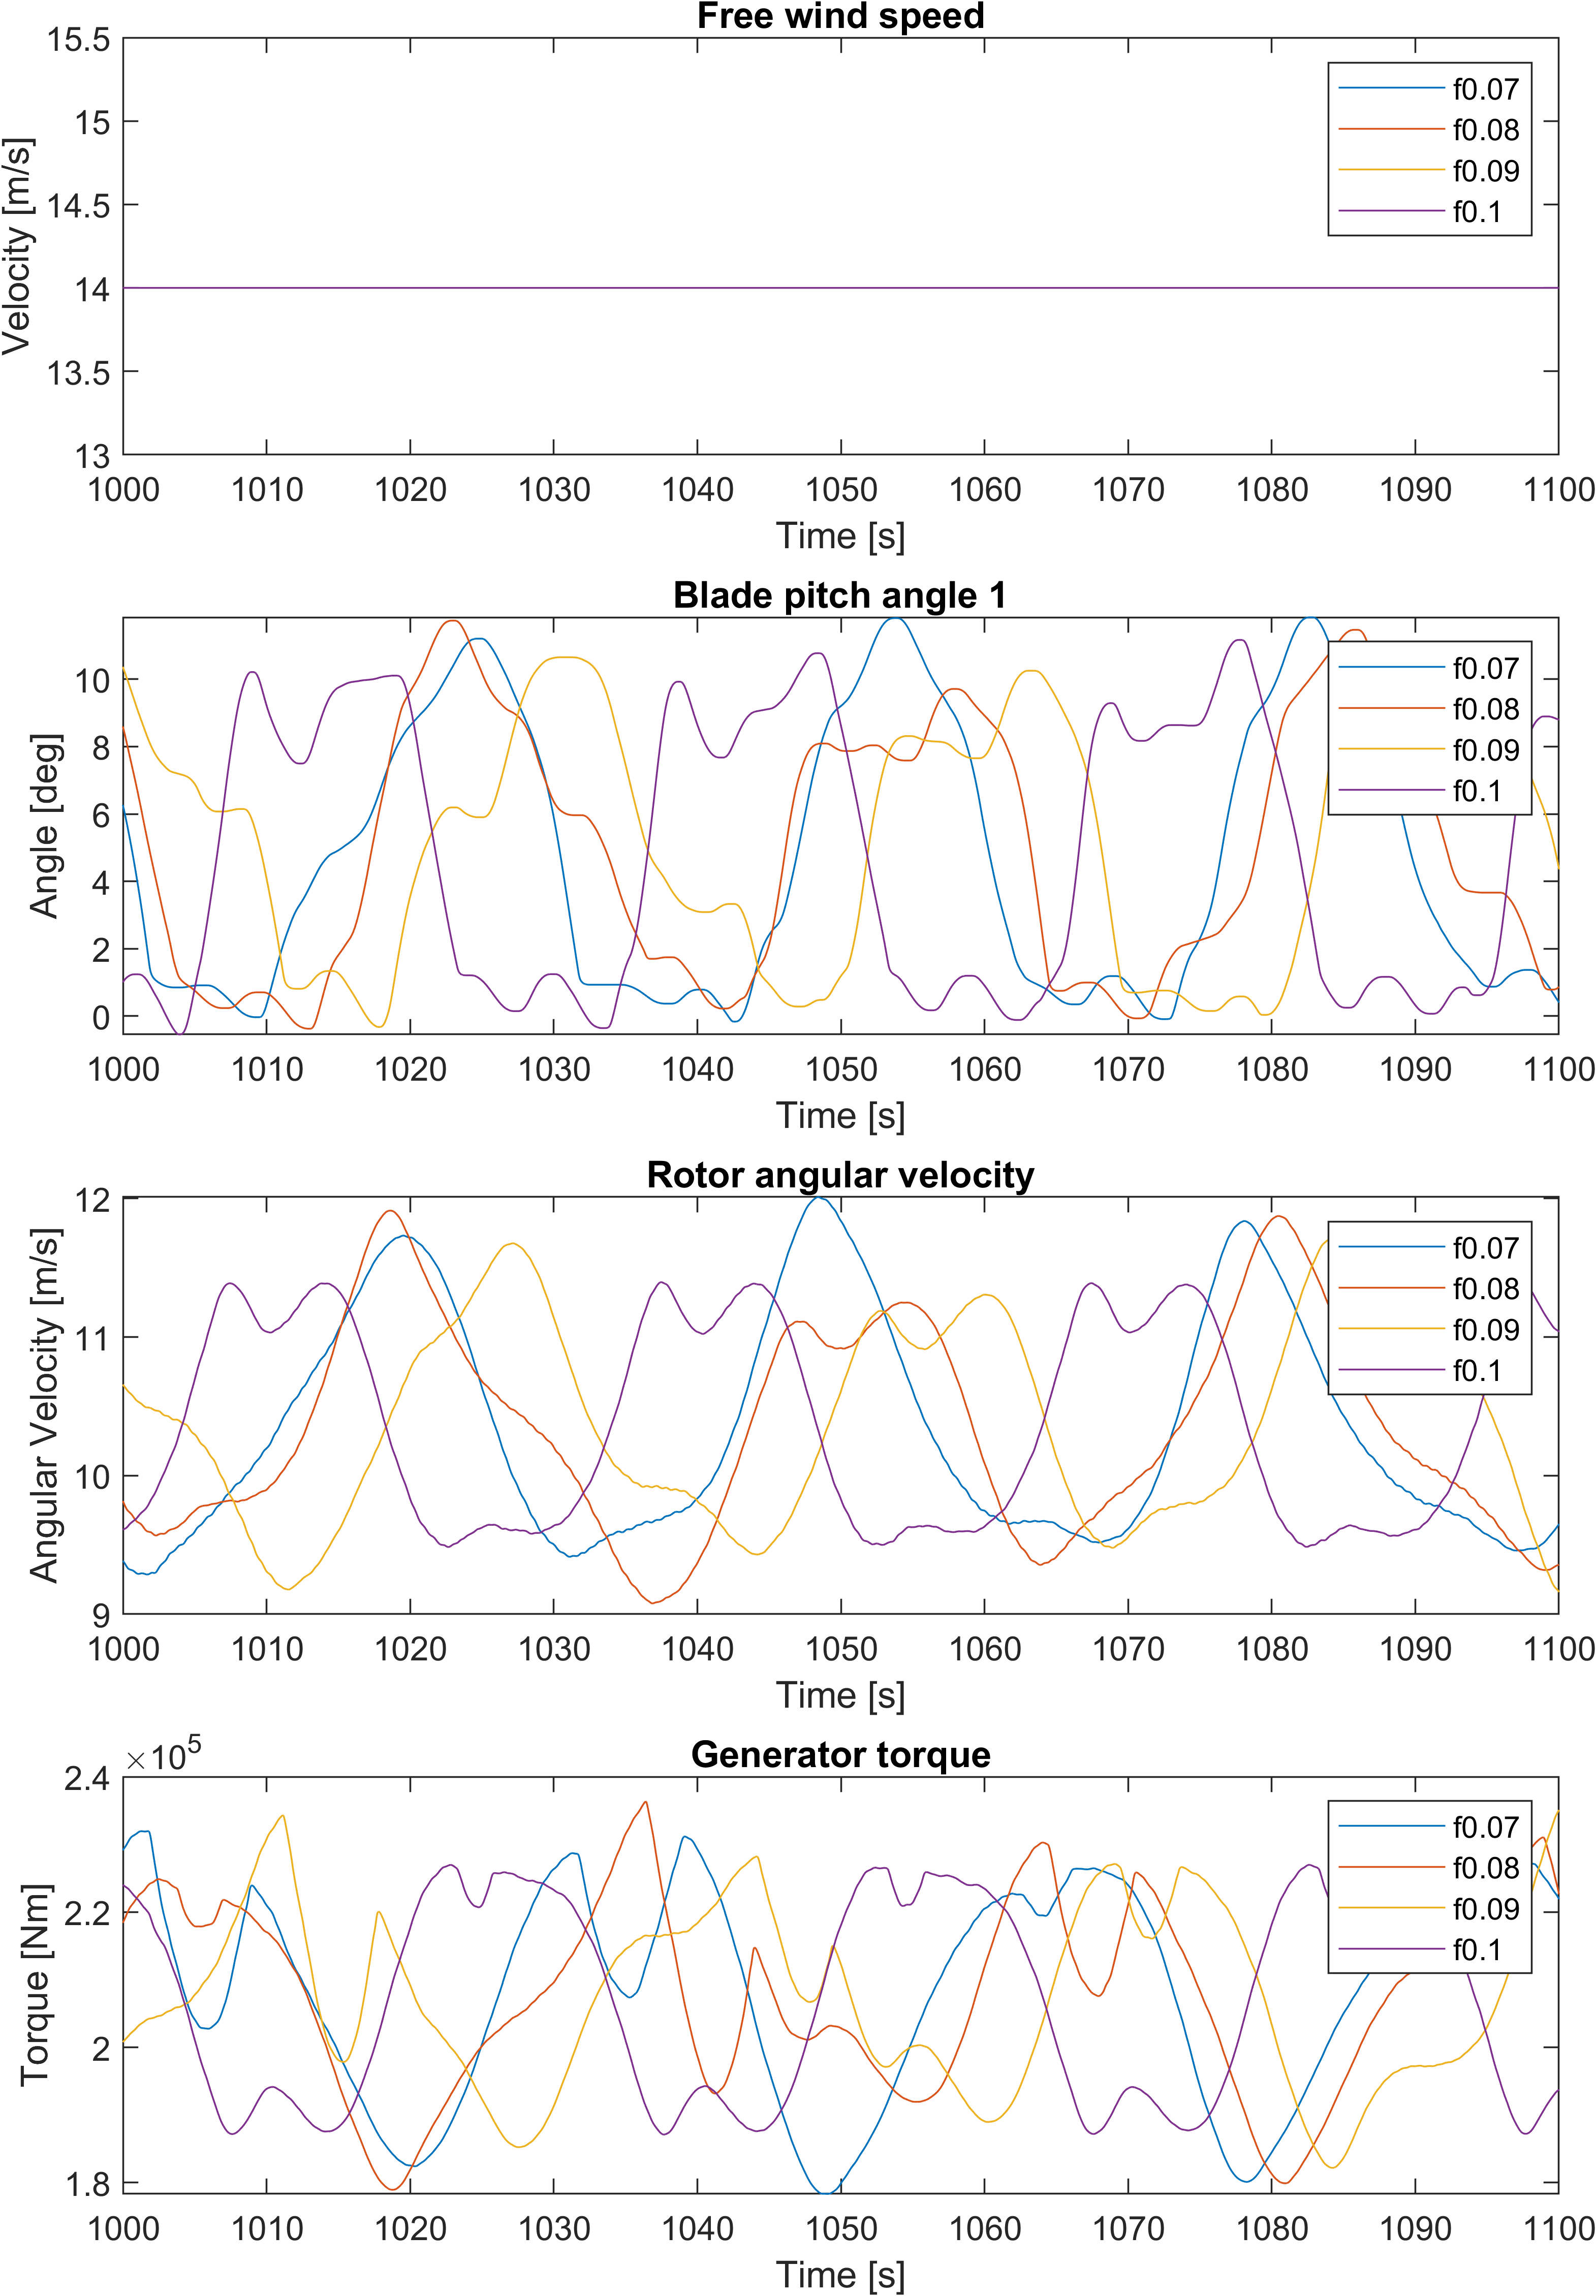
\includegraphics[width=0.8\linewidth]{Graphics/TestResults/tj00/tjj0_f07to1_VfreeToMgen.png}
	\caption{Plot of Free wind, Blade pitch angle 1, rotor angular velocity and Generator torque for the injected rotor angular velocity frequencies 0.07 Hz, 0.08 Hz, 0.09 Hz and 0.1 Hz. It is difficult to observe the frequencies directly on the angular velocity.}
	\label{fig:tjj0_f07to1VfreeToMgen}
\end{figure}

\begin{figure}[h]
	\centering
	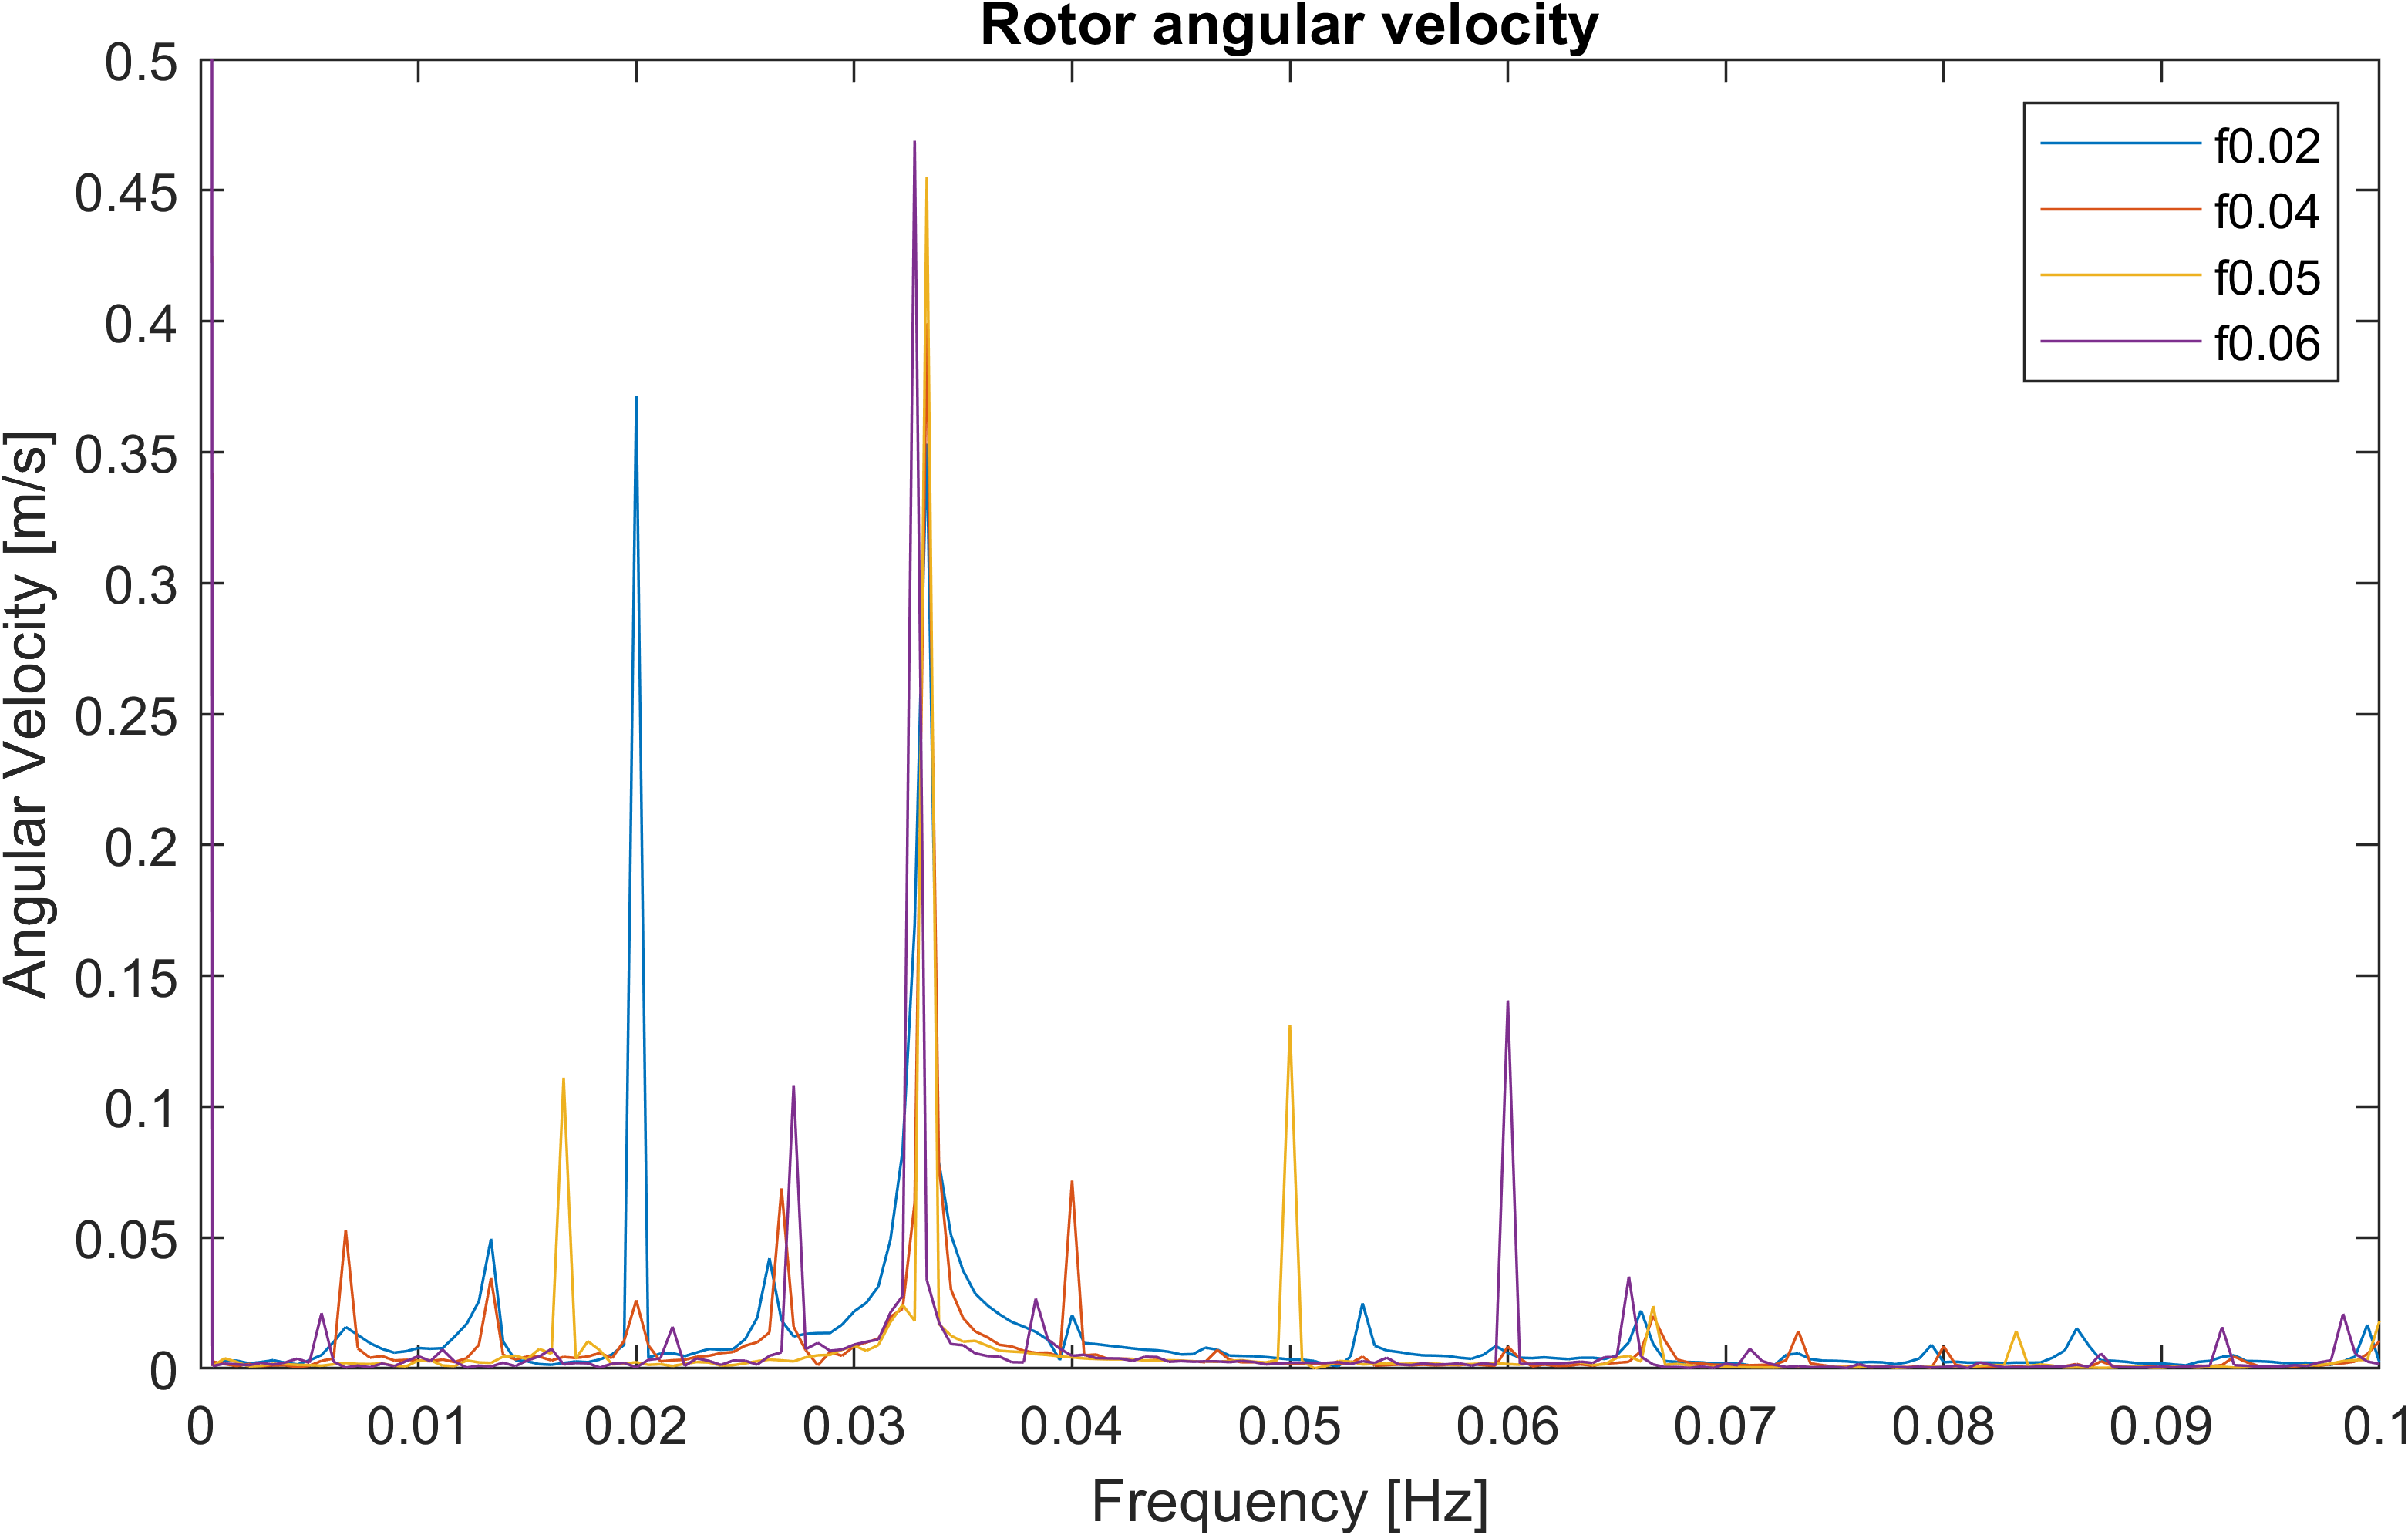
\includegraphics[width=0.8\linewidth]{Graphics/TestResults/tj00/tjj0_f02to06OmegaFFT.png}
	\caption{Plot of FFT of rotor angular velocity for the injected rotor angular velocity frequencies 0.02 Hz, 0.04 Hz, 0.05 Hz and 0.06 Hz. The injected frequencies can be observed as pins at each of the respective frequencies.}
	\label{fig:tjj0_f02to06OmegaFFT}
\end{figure}

\begin{figure}[h]
	\centering
	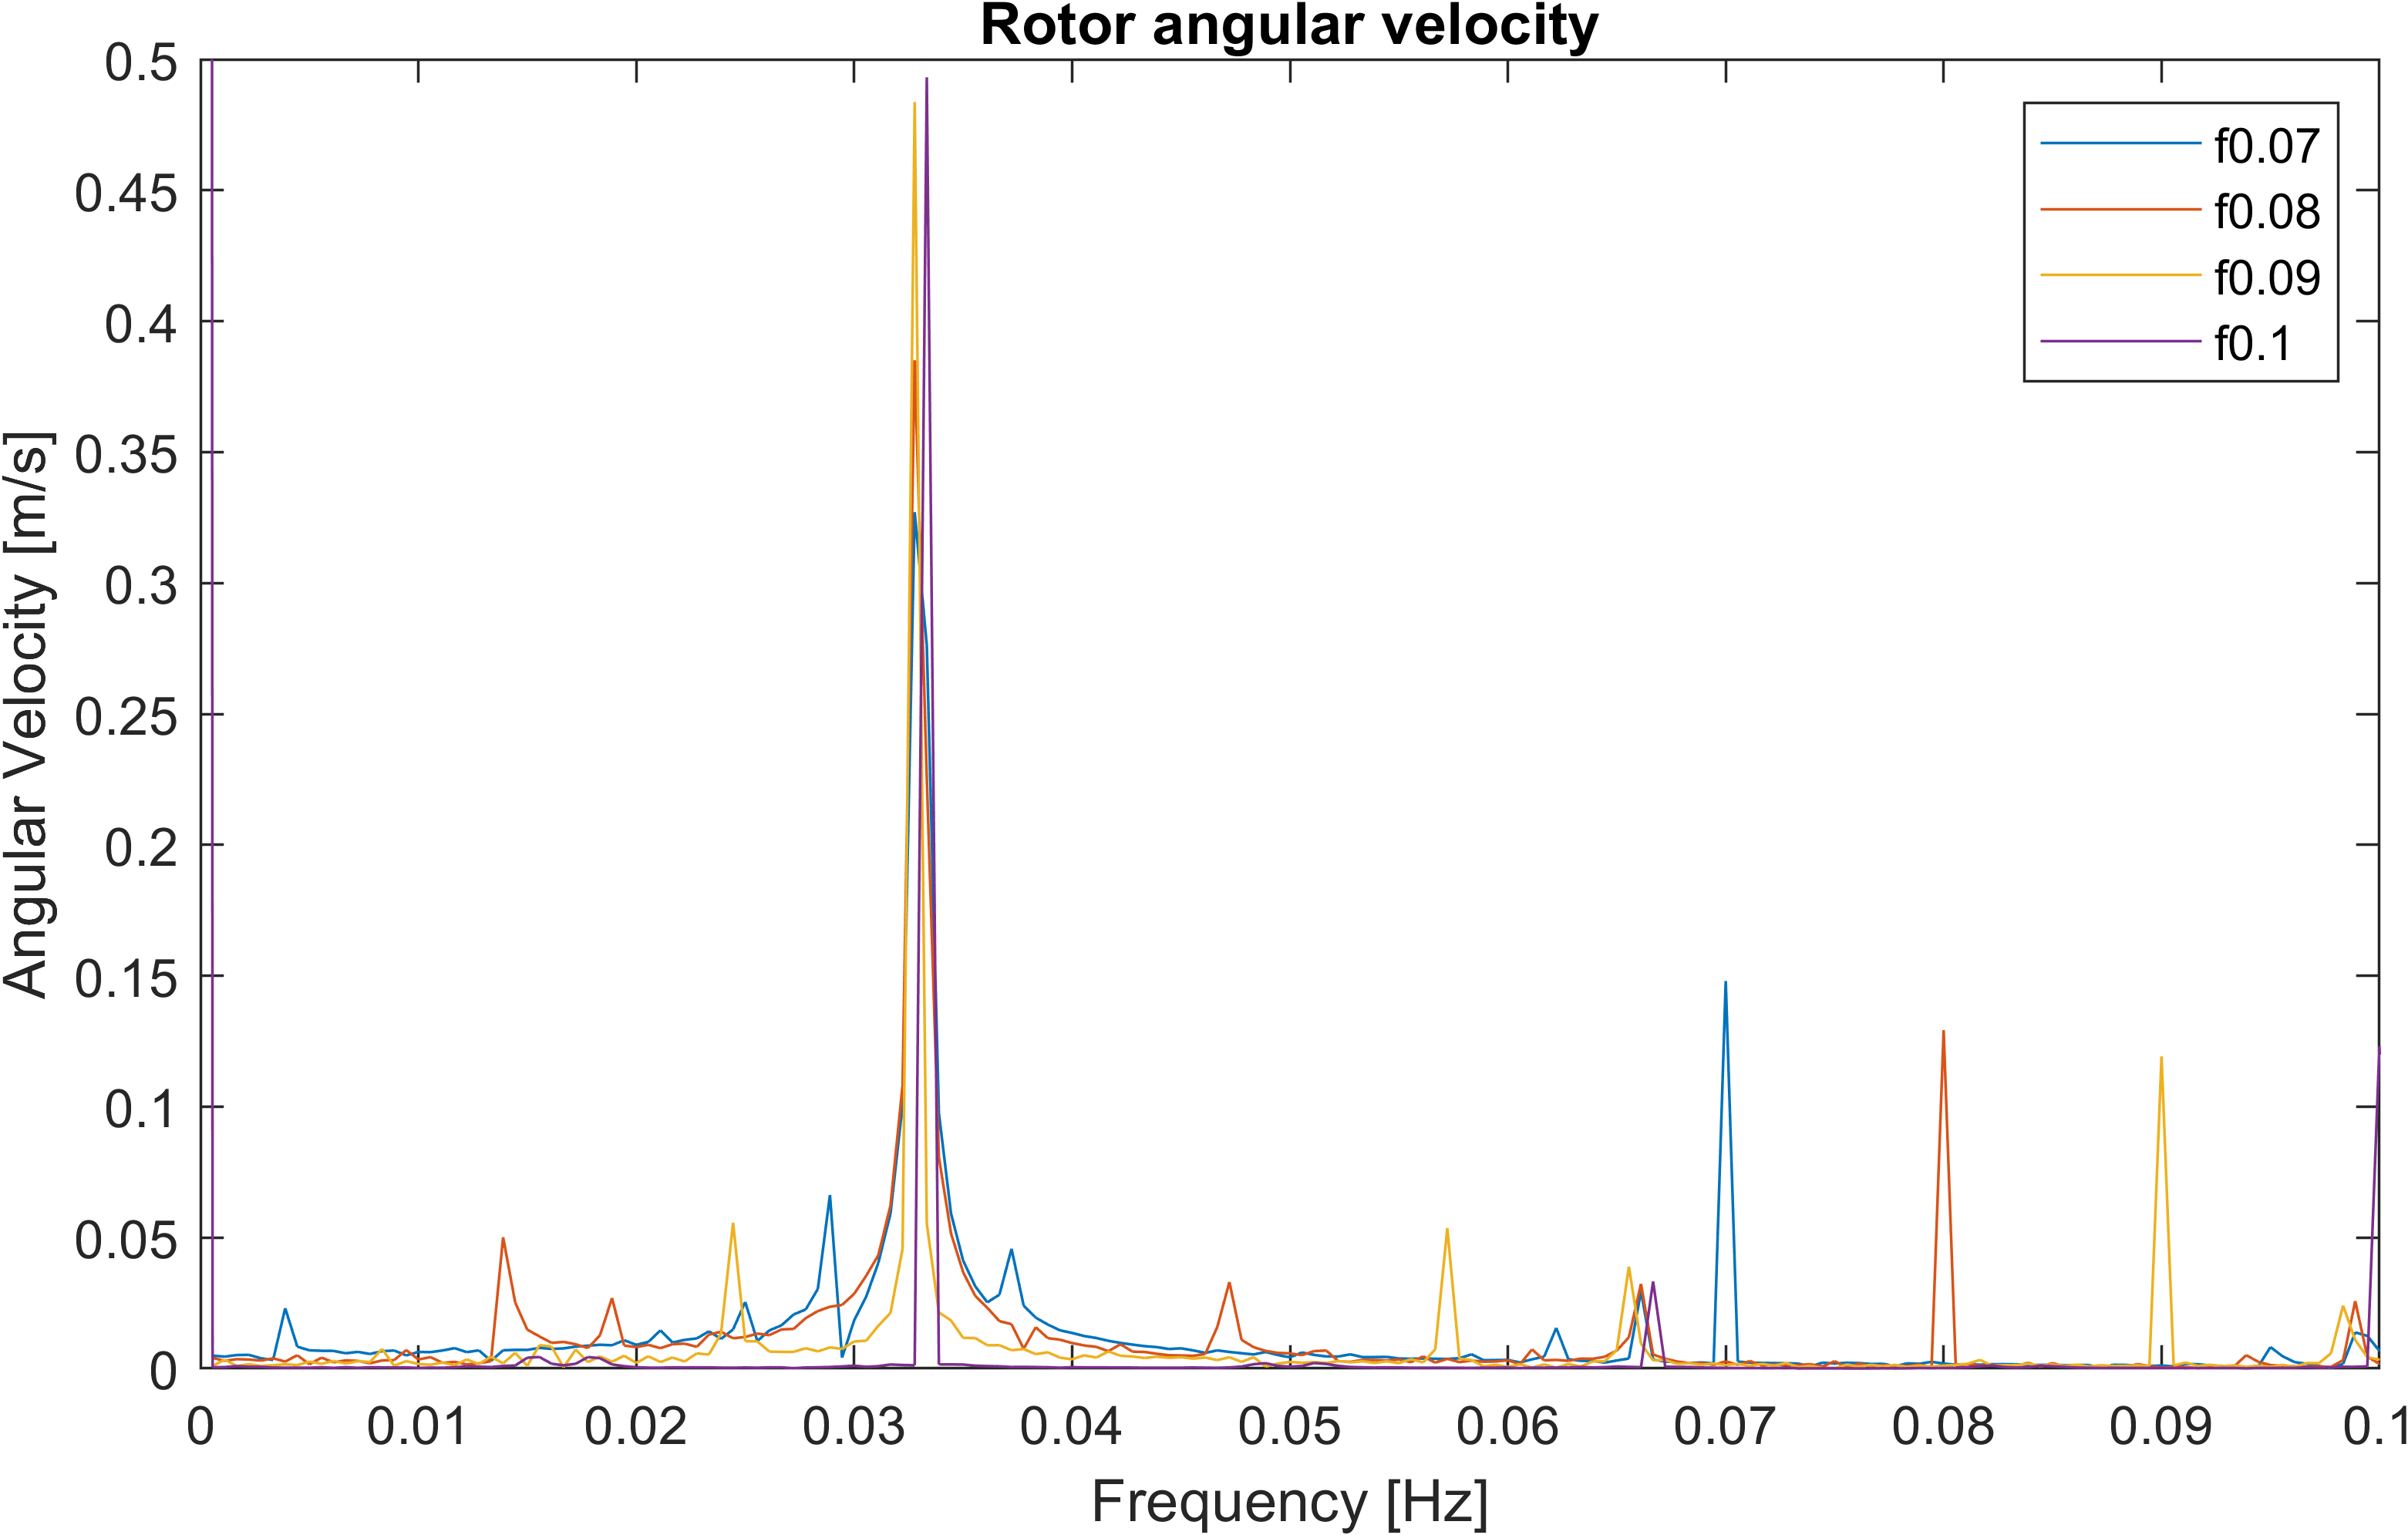
\includegraphics[width=0.8\linewidth]{Graphics/TestResults/tj00/tjj0_f07to1_OmegaFFT.png}
	\caption{Plot of FFT of rotor angular velocity for the injected rotor angular velocity frequencies 0.07 Hz, 0.08 Hz, 0.09 Hz and 0.1 Hz. The injected frequencies can be observed as pins at each of the respective frequencies.}
	\label{fig:tjj0_f07to1_OmegaFFT}
\end{figure}

\begin{figure}[h]
	\centering
	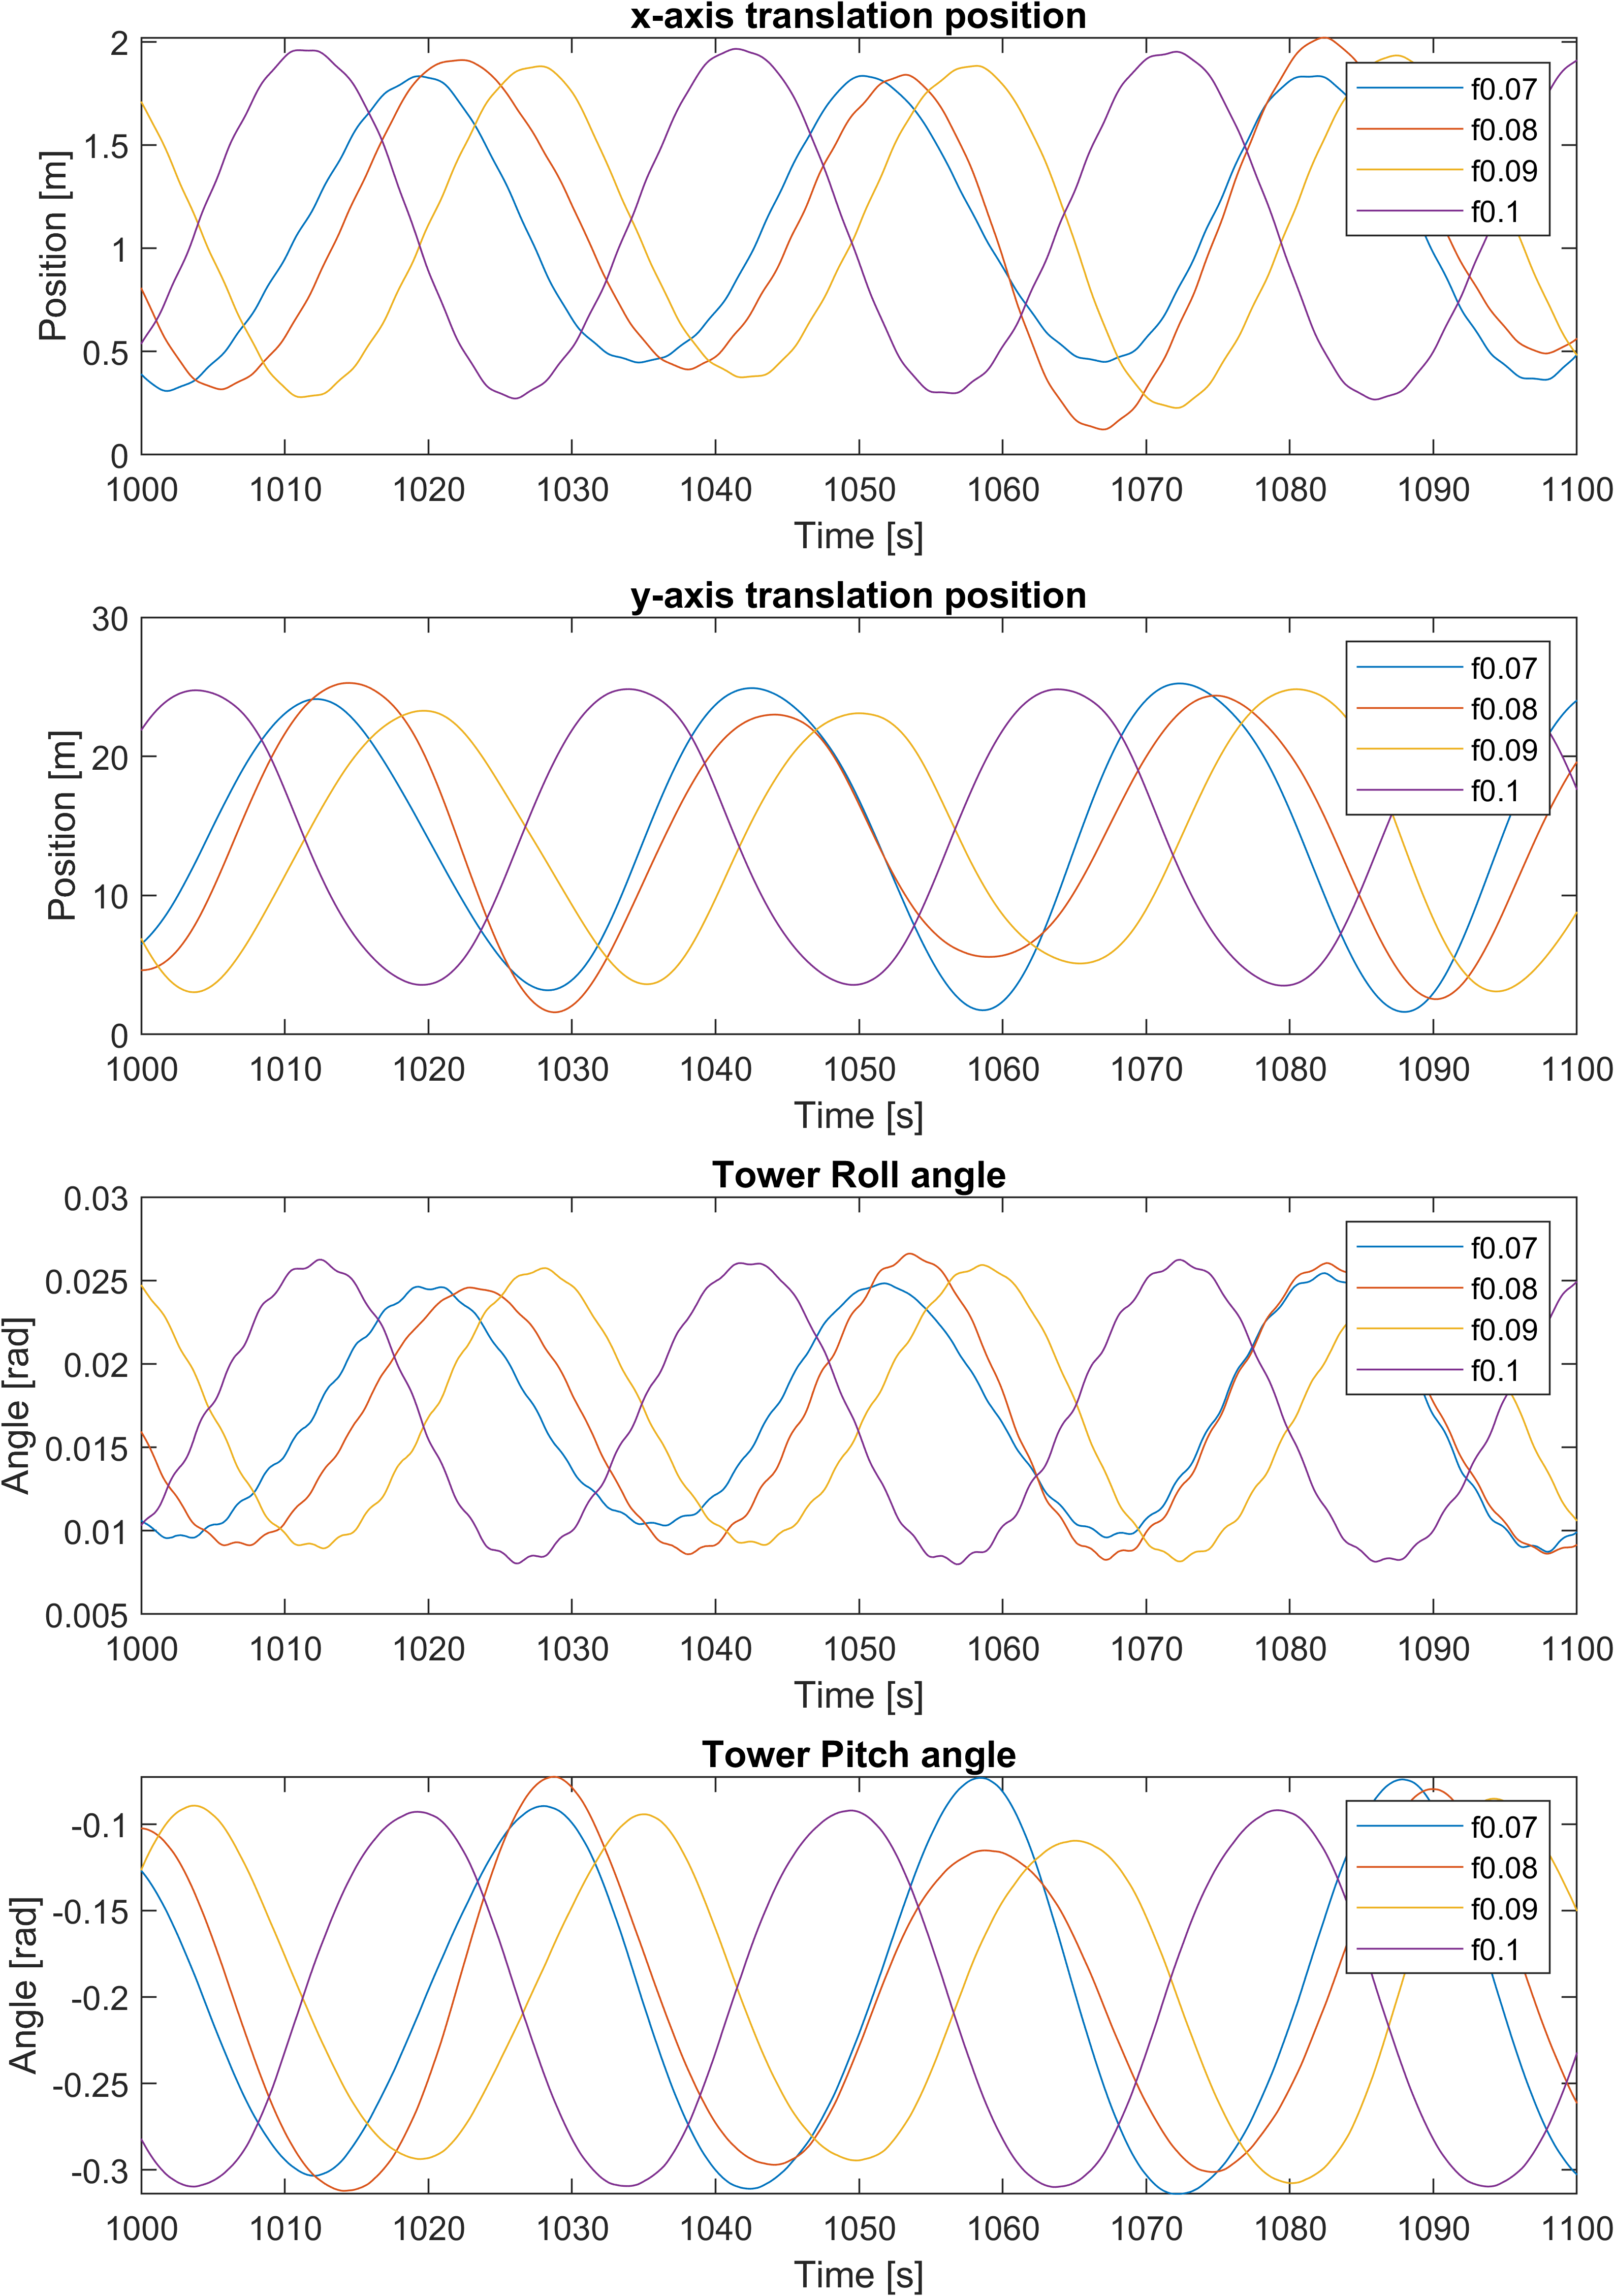
\includegraphics[width=0.8\linewidth]{Graphics/TestResults/tj00/tjj0_f07to1_xPosToPitchAng.png}
	\caption{Plot of x- and y-axis translation position and tower roll and pitch angle for the injected rotor angular velocity frequencies 0.07 Hz, 0.08 Hz, 0.09 Hz and 0.1 Hz. The natural frequency of the turbine in the water is apparent in both the translation and pitch.}
	\label{fig:tjj0_f07to1_xPosToPitchAng}
\end{figure}

\begin{figure}[h]
	\centering
	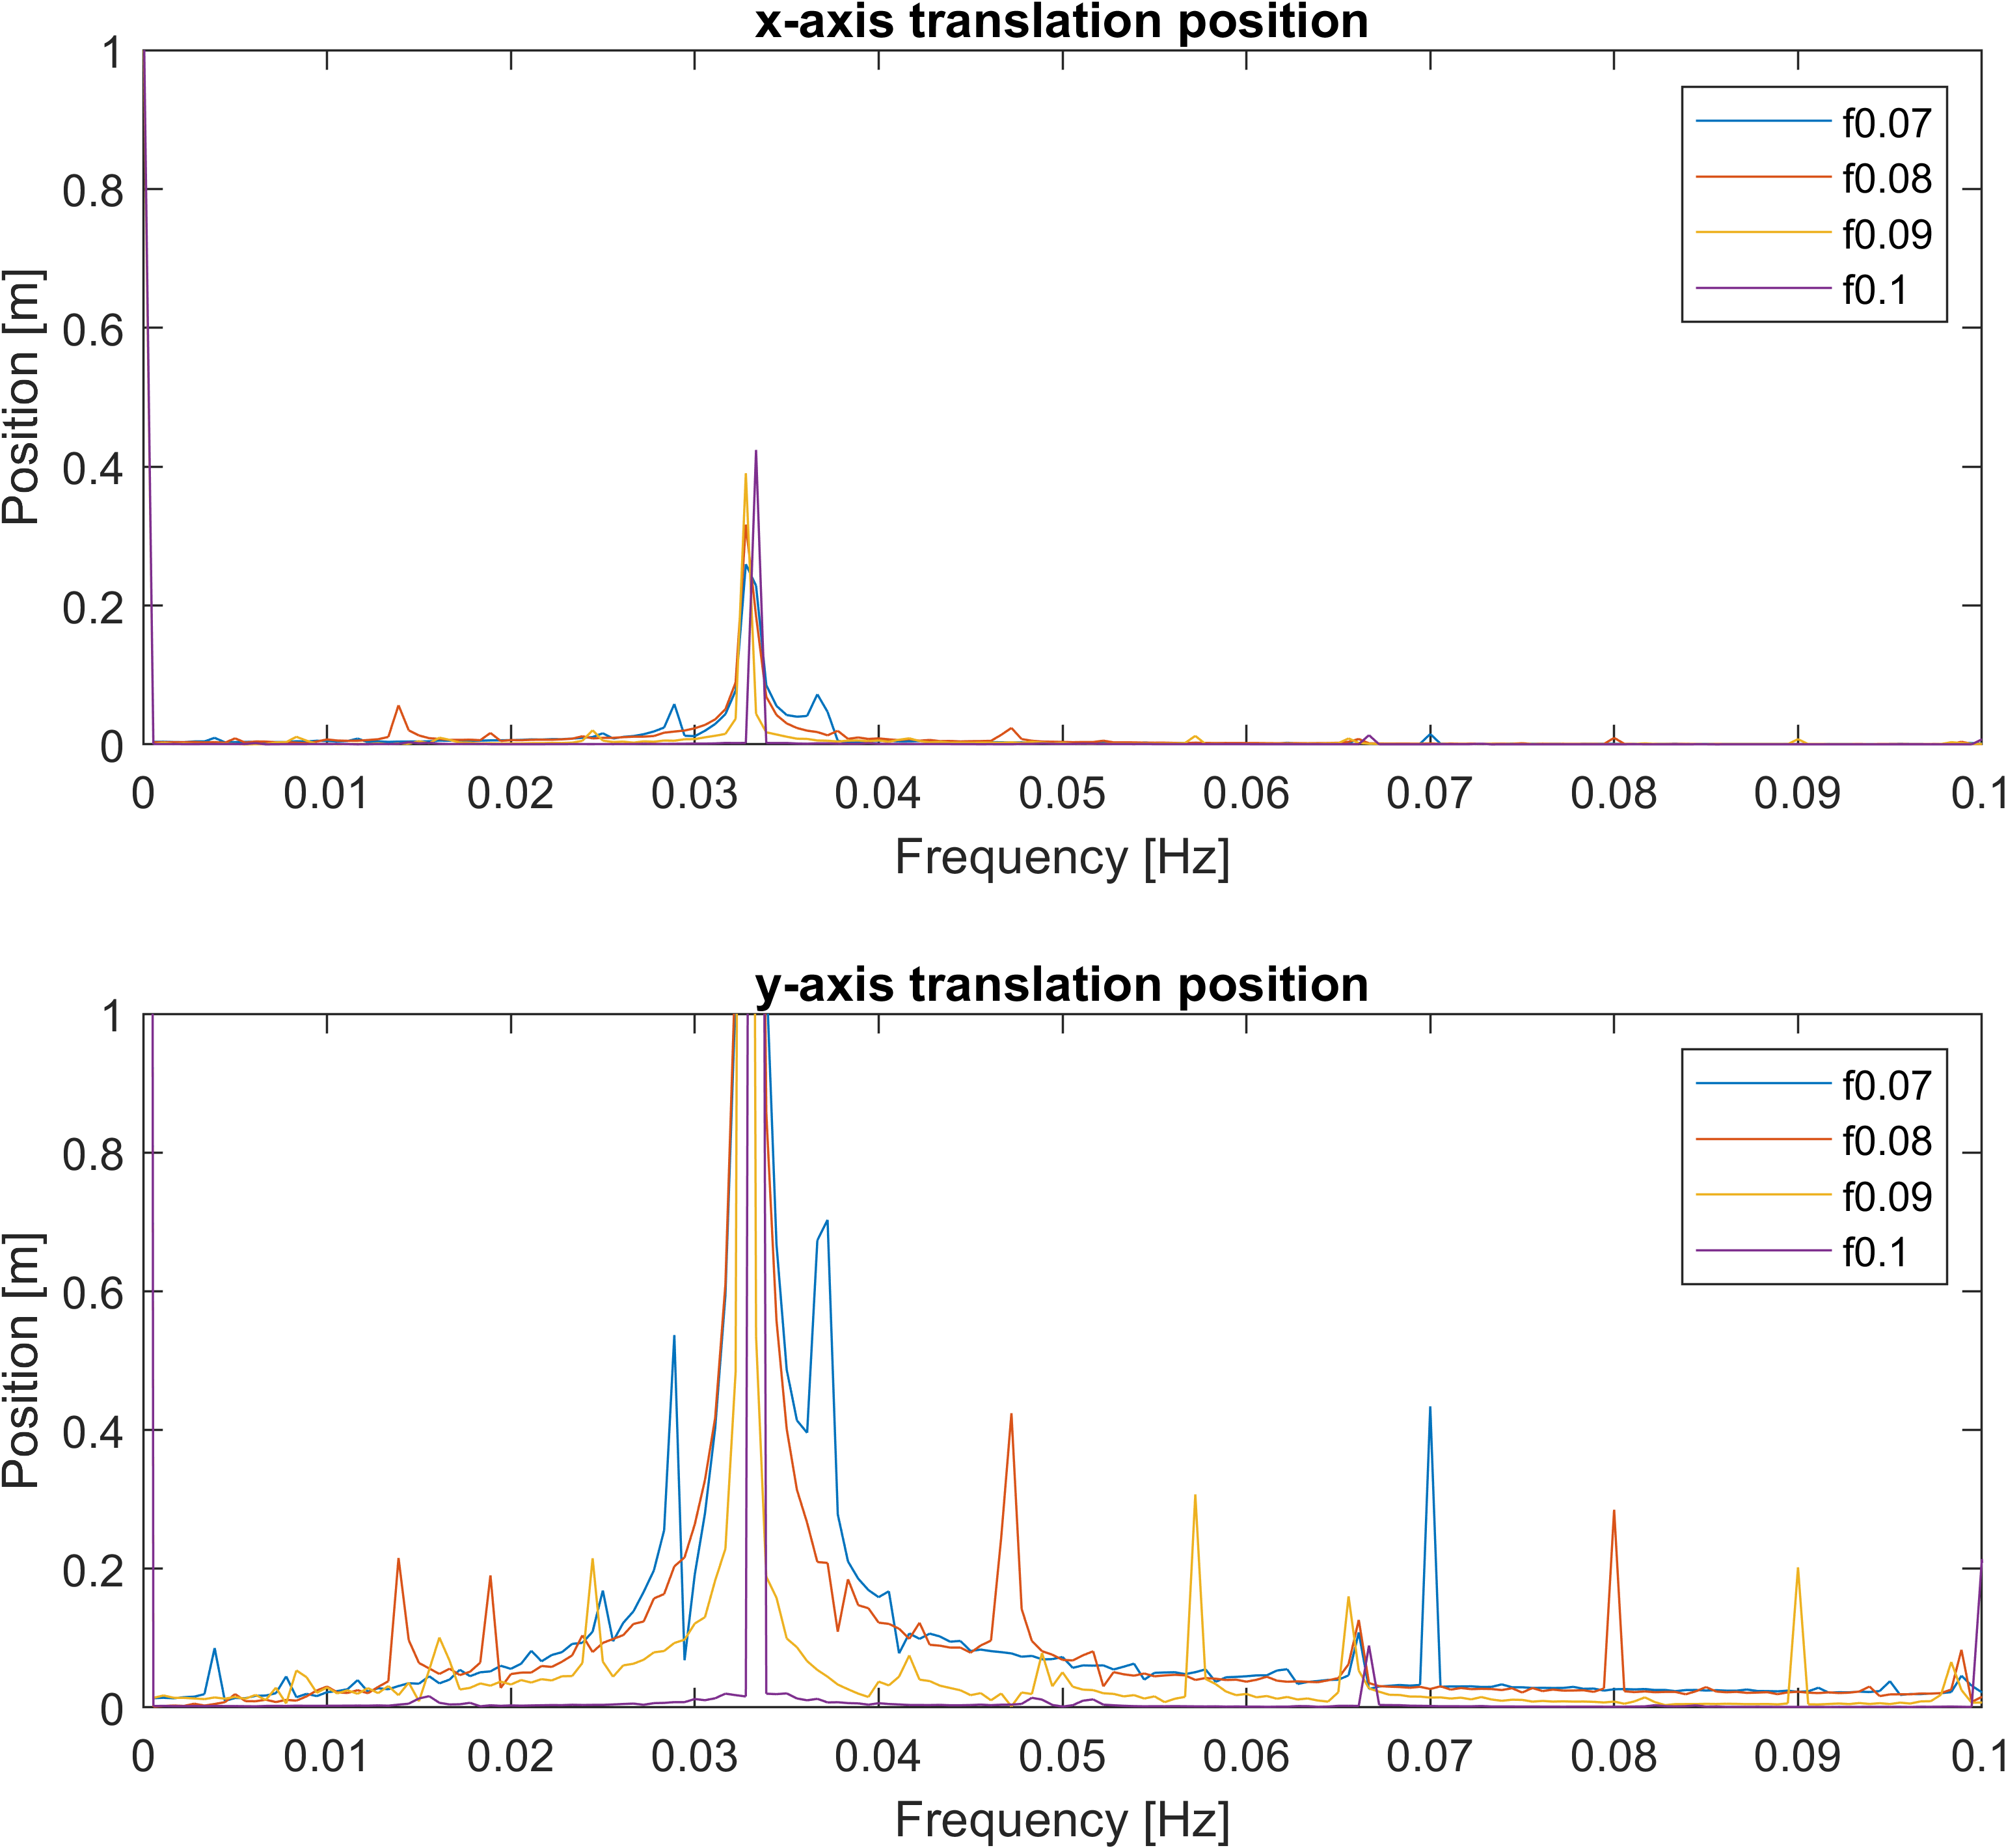
\includegraphics[width=0.8\linewidth]{Graphics/TestResults/tj00/tjj0_f07to1_xPosyPosFFT.png}
	\caption{Plot of FFT of x- and y-axis translation position for the injected rotor angular velocity frequencies 0.07 Hz, 0.08 Hz, 0.09 Hz and 0.1 Hz. The natural frequency of the turbine is greatly apparent around 0.034 Hz especially in the y-translation position subplot. The injected frequencies are visible at their respective frequencies, especially for the y-axis translation position. It is also visible that lower frequencies are translated better.}
	\label{fig:tjj0_f07to1_xPosyPosFFT}
\end{figure}

\begin{figure}[h]
	\centering
	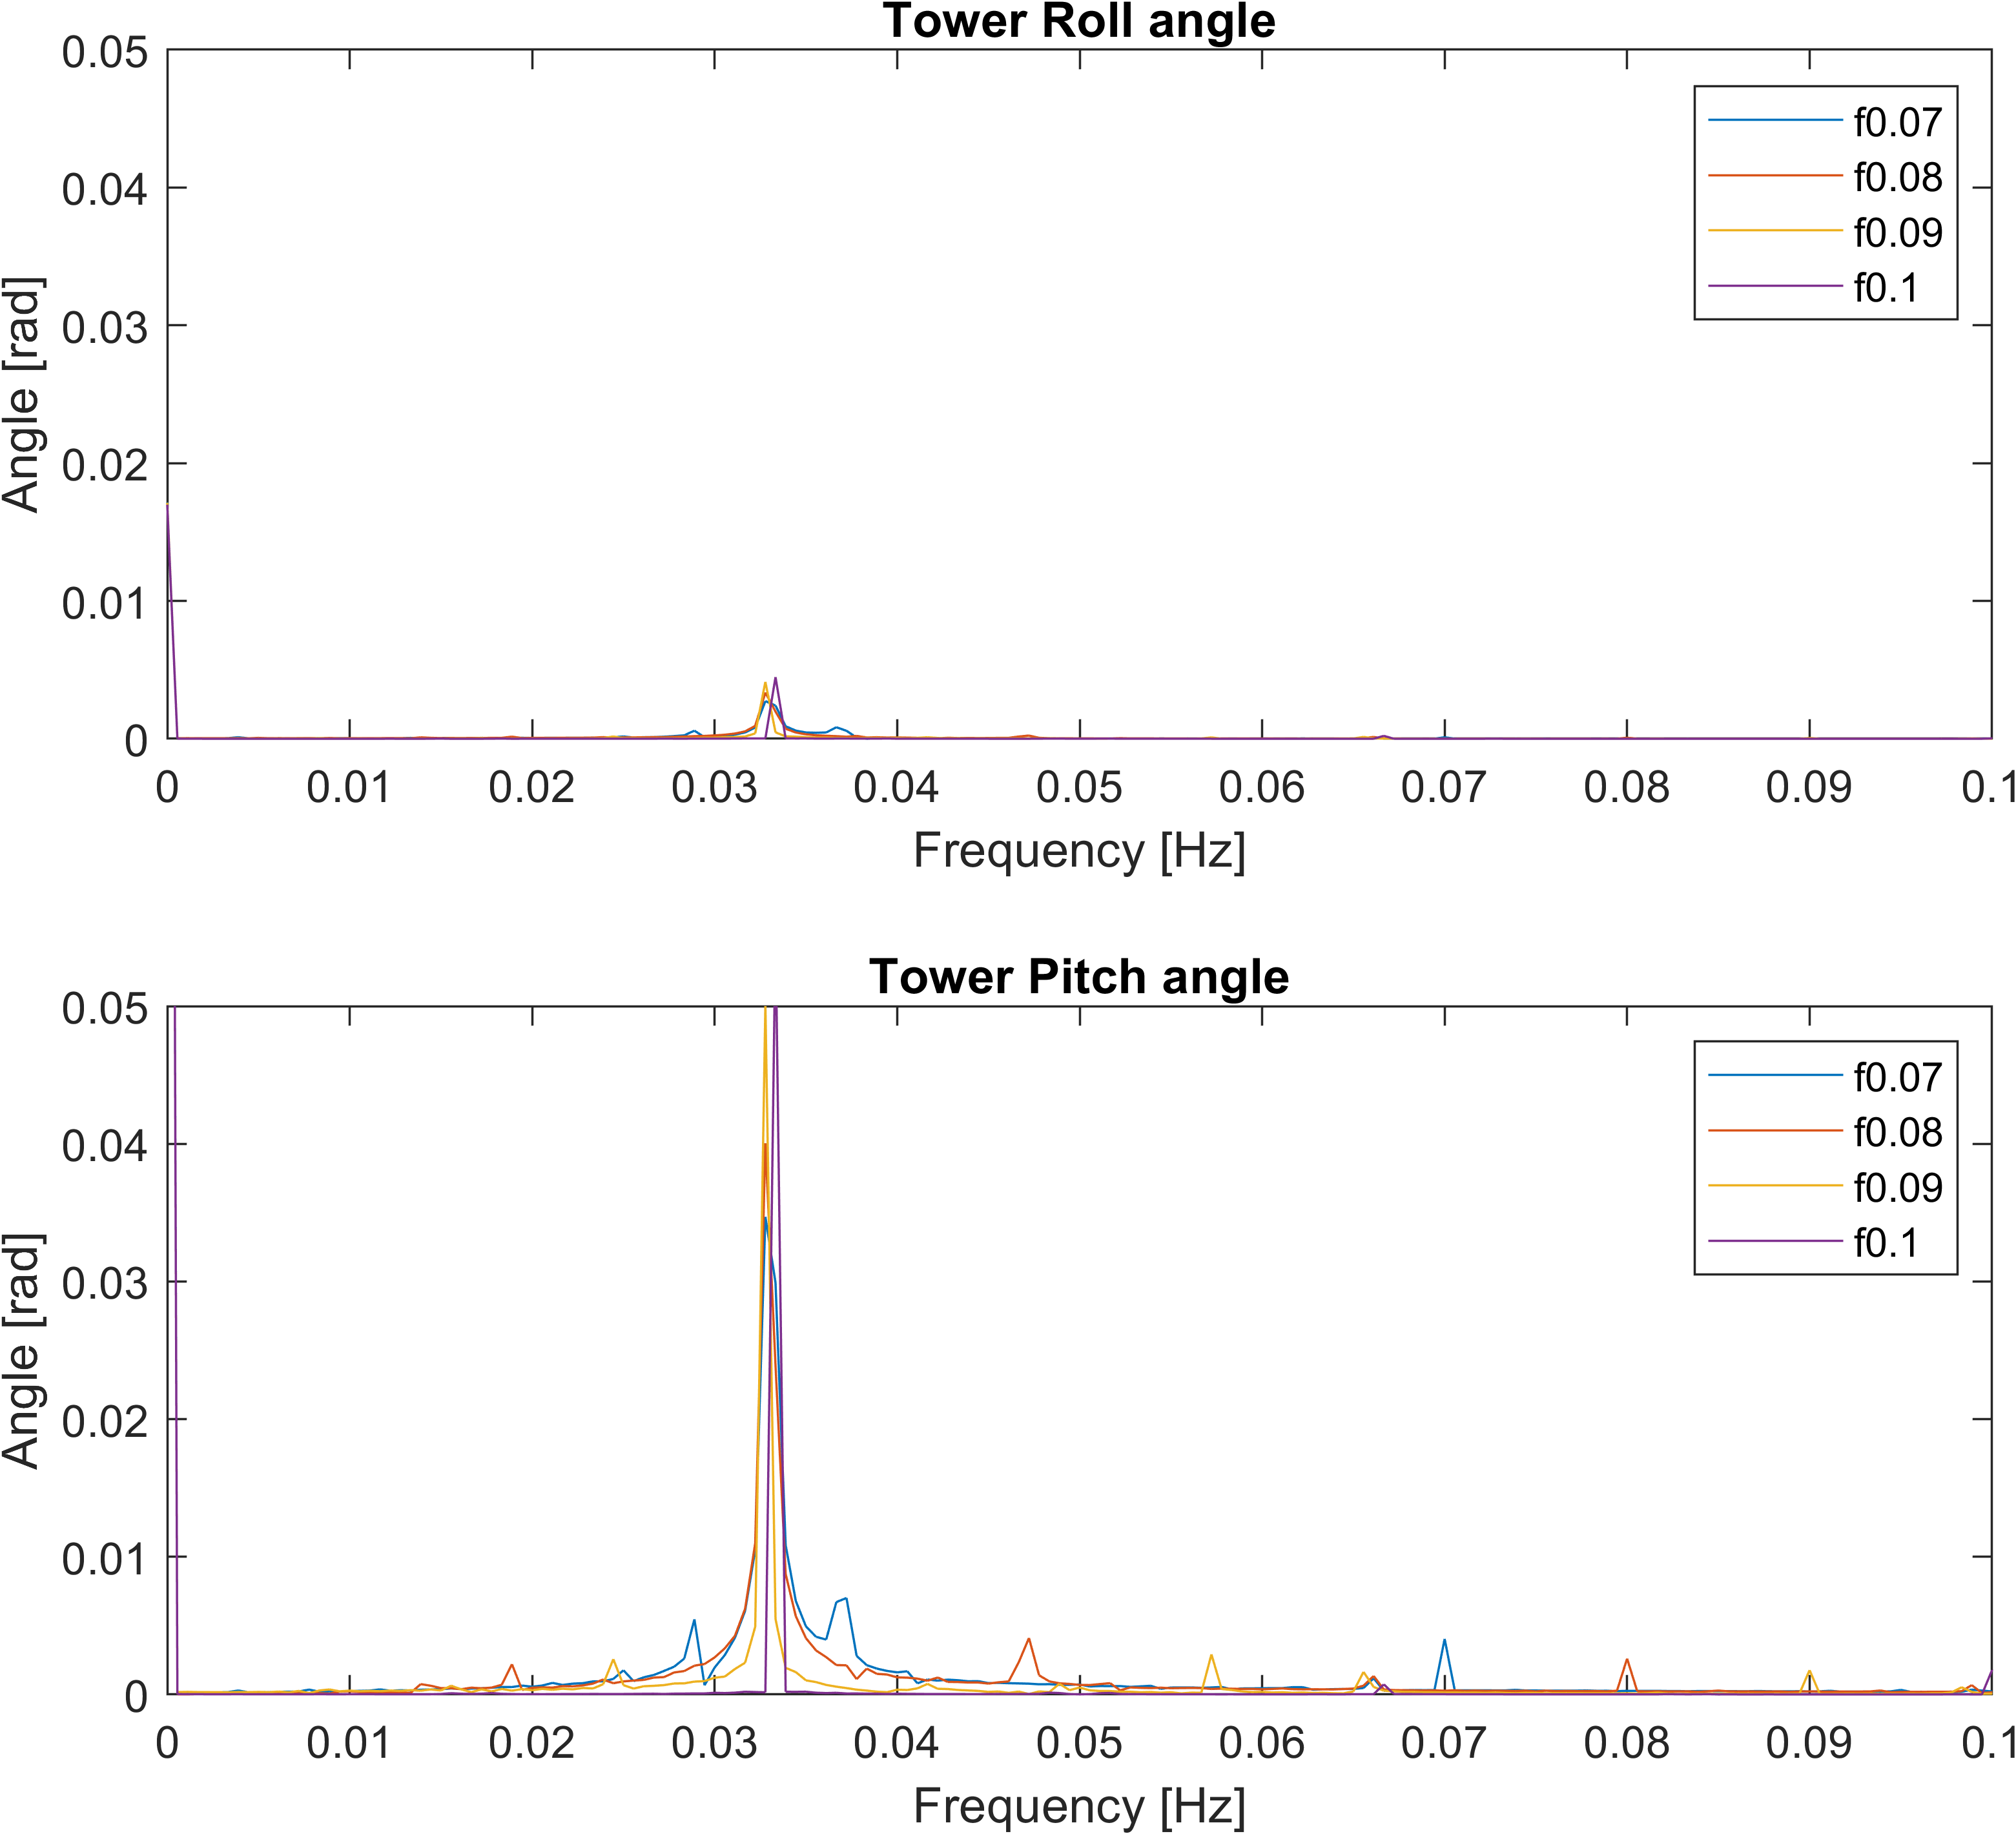
\includegraphics[width=0.8\linewidth]{Graphics/TestResults/tj00/tjj0_f07to1_RollPitchAngFFT.png}
	\caption{Plot of FFT of roll and pitch angle for the injected rotor angular velocity frequencies 0.07 Hz, 0.08 Hz, 0.09 Hz and 0.1 Hz. The natural frequency of the turbine is greatly apparent around 0.034 Hz especially in the pitch angle. The injected frequencies are visible at their respective frequencies, especially for the pitch angle. It is also visible that lower frequencies are translated better.}
	\label{fig:tjj0_f07to1_RollPitchAngFFT}
\end{figure}

%\begin{figure}[h]
%	\centering
%	\includegraphics[width=0.8\linewidth]{Graphics/TestResults/tj00/}
%	\caption{}
%	\label{fig:tj00_}
%\end{figure}
%
%\begin{figure}[h]
%	\centering
%	\includegraphics[width=0.8\linewidth]{Graphics/TestResults/tj00/}
%	\caption{}
%	\label{fig:tj00_}
%\end{figure}


\subsubsection{Sources of error and insecurities}


% trigger a \newpage just before the given reference
% number - used to balance the columns on the last page
% adjust value as needed - may need to be readjusted if
% the document is modified later
%\IEEEtriggeratref{8}
% The "triggered" command can be changed if desired:
%\IEEEtriggercmd{\enlargethispage{-5in}}

% references section

% can use a generated by BibTeX as a .bbl file
% BibTeX documentation can be easily obtained at:
% http://mirror.ctan.org/biblio/bibtex/contrib/doc/
% The IEEEtran BibTeX style support page is at:
% http://www.michaelshell.org/tex/ieeetran/bibtex/
%\bibliographystyle{IEEEtran}
% argument is your BibTeX string definitions and bibliography database(s)
%\bibliography{IEEEabrv,../bib/paper}
%
% <OR> manually copy in the resultant .bbl file
% set second argument of \begin to the number of references
% (used to reserve space for the reference number labels box)


% that's all folks
\end{document}

	
